\chapter{Clustering of Pin-Wise MGXS}
\label{chap:spatial}

The preceding chapter quantified the benefit of using degenerate spatial homogenization to predict pin-wise U-238 capture rates as accurately as fission rates in high-fidelity multi-group transport methods. However, it was also noted that the degenerate scheme requires far more Monte Carlo particle histories to converge \ac{MGXS} tallies than are necessary for the simpler null or infinite schemes. In addition, orders of magnitude more memory is needed to store \ac{MGXS} libraries produced from degenerate homogenization. These observations motivate the need for a more sophisticated approach to pin-wise spatial homogenization which can simultaneously achieve nearly the accuracy of degenerate homogenization and the convergence of null homogenization.

This chapter seeks to accomplish this by leveraging the finding from Chap.~\ref{chap:quantify} that pins with similar neighboring heterogeneities generally have similar reaction rate errors. For example, null homogenization led to a structured spatial distribution of errors with systematically similar errors in pins facially adjacent to one or two \acp{CRGT}, \acp{BP}, along inter-assembly and assembly-reflector interfaces, and so on. Since degenerate homogenization largely erased this structural error distribution, it follows that pins with similar errors likely experience similar spatial self-shielding effects due to neighboring heterogeneities. As a result, this and the following chapters develop the hypothesis that \textbf{pins with similar neighboring heterogeneities have similar microscopic \ac{MGXS}}. If pins with similar microscopic \ac{MGXS} can be identified, the \ac{MGXS} tallied in these pin instances may be \textit{homogenized} to compute an estimate which is nearly as accurate as the \ac{MGXS} from degenerate homogenization, and nearly as converged as the \ac{MGXS} from null homogenization. 

This chapter investigates this hypothesis by analyzing the pin-wise \ac{MGXS} tallied with OpenMC to identify patterns -- namely, clustering -- for pins with similar neighbors. Furthermore, this chapter develops and quantifies a new spatial homogenization technique which analyzes a core geometry to predict which fuel pin instances have similar microscopic \ac{MGXS} due to neighboring heterogeneities. This technique applies OpenCG's Local Neighbor Symmetry algorithm to generate a ``geometric template'' of fuel pins and averages the \ac{MGXS} for pins across a core geometry with the same \ac{LNS} identifiers. The impact of using \ac{LNS} homogenization is compared to the null and degenerate schemes with respect to both general predictive accuracy as well as convergence. The results presented for \ac{LNS} homogenization underscore the promise for an approach which combines the benefits of the null and degenerate schemes. However, the results also highlight some notable shortcomings to \ac{LNS} which motivates the need for an unsupervised approach to \ac{MGXS} clustering, as developed in the following chapter.

This chapter begins by analyzing patterns in visualizations of pin-wise \ac{MGXS} in Sec.~\ref{sec:chap9-clustering}. This includes a case study of the statistical uncertainties and population variance of pin-wise \ac{MGXS} in Secs.~\ref{subsec:chap9-mgxs-uncertainty} and~\ref{subsec:chap9-pop-var}, and an analysis of the distributions of U-235 fission and U-238 capture \ac{MGXS} for each of the six heterogeneous benchmarks with histograms and quantile-quantile plots in Secs.~\ref{subsec:chap9-histograms} and ~\ref{subsec:chap9-qq-plots}, respectively. A new spatial homogenization scheme based upon OpenCG's \ac{LNS} algorithm is introduced in Sec.~\ref{sec:chap9-lns-homogenize}. The OpenMOC eigenvalues and pin-wise fission and U-238 capture rates with \ac{LNS} spatial homogenization are presented in Sec.~\ref{sec:chap9-lns-results}. Finally, the statistical uncertainties and convergence rate for \ac{MGXS} generated with the null, degenerate and \ac{LNS} schemes are compared in Sec.~\ref{sec:chap9-convergence}.


%%%%%%%%%%%%%%%%%%%%%%%%%%%%%%%%%%%%%%%%%%%%%%%%%%%%%%%%%%%%%%%%%%%%%%%%%%%%%%%
\section{Clustering of Pin-Wise MGXS}
\label{sec:chap9-clustering}

This section investigates the clustering of pin-wise \ac{MGXS} due to spatial self-shielding effects induced by neighboring heterogeneities. As a thought experiment, consider the pin-wise \ac{MGXS} in an infinite lattice\footnote{An infinitely repeating lattice of identical fuel pins.}. Although the pin-wise \ac{MGXS} in such a uniform geometry are necessarily identical, due to the stochastic nature of \ac{MC}, the population of pin-wise \ac{MGXS} estimates from \ac{MC} will have a non-zero variance and represent random variates drawn from a normal distribution. When heterogeneities such as \acp{CRGT} and \acp{BP} are introduced into the geometry, they will induce local spatial self-shielding effects on nearby pins. As a result, the population of pin-wise \ac{MGXS} will no longer be drawn from a simple normal distribution, but rather some mixture of potentially more complicated distributions. As shown in this section, such deviations may be observed from the population of pin-wise microscopic \ac{MGXS} tallied with \ac{MC}.

It is important to note that self-shielding effects induce clustering of microscopic rather than macroscopic \ac{MGXS}. The pin-wise macroscopic \ac{MGXS} cluster (or disperse) due to the different densities of nuclides in each fuel pin and give no indication of the similarity of the spectra experienced by each fuel pin. Since all of the benchmarks in this thesis use an isotopic vector for fresh \ac{PWR} fuel, the clustering effects investigated here are necessarily the same for both micro and macro \ac{MGXS}. However, the spatial homogenization methods developed in this thesis are intended to be used for more general applications with fuels of various burnups. Hence this section analyzes the microscopic \ac{MGXS} since this is most appropriate for general purpose \ac{MGXS} generation.

This section quantifies and visualizes the impact of heterogeneities on pin-wise \ac{MGXS}. The \ac{MGXS} data analyzed in this section was produced from the OpenMC simulations used to compute \ac{MGXS} for Chap.~\ref{chap:quantify} for degenerate homogenization. Sec.~\ref{subsec:chap9-mgxs-uncertainty} begins by briefly quantifying the statistical uncertainties for the tallied \ac{MGXS} datasets. Sec.~\ref{subsec:chap9-pop-var} investigates the population variance of \ac{MGXS} for each of the heterogeneous benchmarks and compares it to data for an infinite lattice\footnote{A 17$\times$17 assembly of identical fuel pins with reflective boundary conditions. The \ac{MGXS} are tallied separately in each of the 289 identical fuel pins.}. Secs.~\ref{subsec:chap9-histograms} and~\ref{subsec:chap9-qq-plots} analyze histograms and quantile-quantile plots of the distribution of pin-wise \ac{MGXS} for each of the benchmarks, respectively. Although the preceding chapter identified U-238 capture rates as being more sensitive to the pin-wise spatial homogenization model than the fission rates, this section explores both U-238 capture and U-235 fission \ac{MGXS} data. As observed in the following chapters, the clustering of one nuclide or reaction type's \ac{MGXS} may not have a sizable impact on the corresponding reaction rate distribution (\textit{e.g.}, fission), but may still reflect spatial self-shielding effects which can be leveraged to better predict other reaction rate distributions.

%%%%%%%%%%%%%%%%%%%%%%%%%%%%%%%%%%%%%%%%%%%%%%%%%%
\subsection{Pin-Wise MGXS Statistical Uncertainty}
\label{subsec:chap9-mgxs-uncertainty}

Before investigating \ac{MGXS} clustering, it is important to first quantify the statistical uncertainties of the tallied pin-wise \ac{MGXS} for each benchmark. The max and mean relative uncertainties\footnote{The \textit{relative uncertainty} as used here is defined as the standard deviation of the sample mean divided by the sample mean.} of the pin-wise U-238 capture and U-235 fission \ac{MGXS} for an infinite lattice and each of the heterogeneous benchmarks are presented in Tab.~\ref{table:chap9-std-dev-mgxs}. The standard deviations were computed by propagating the standard deviations of the reaction rate and flux tallies (Eqn.~\ref{eqn:chap3-variance-mean}) as discussed in Sec.~\ref{subsec:chap3-uncertainty-prop}. The standard deviations were computed for all of the pins in each benchmark, and the max and mean values were selected for the table. The table highlights the standard deviations for both 1.6\% and 3.1\% enriched fuel pins\footnote{Although the \ac{BEAVRS} model includes 2.4\% enriched fuel pins, they were not included in this analysis.}. The \ac{MGXS} data was computed in two energy groups. The U-238 capture \ac{MGXS} is analyzed for the first (fast) energy group since it encompasses the resonance region which is most sensitive to spatial self-shielding effects. The U-235 fission \ac{MGXS} is analyzed for the second (thermal) energy group since it encompasses thermal energies which drives the majority of fission in \acp{LWR}.

There are a few key observations which can be made from the statistical uncertainties. First, the statistical uncertainties for both \ac{MGXS} are relatively small with respect to the means. In particular, the relative uncertainties are 0.1 -- 0.75\% and 0.05 -- 0.25\% for the U-238 capture and U-235 fission \ac{MGXS}, respectively. Furthermore, the reported standard deviations are likely overestimates since the reaction rate and flux tallies used to compute each \ac{MGXS} are positively correlated (see Sec.~\ref{table:chap9-std-dev-mgxs}). Therefore, the clustering of \ac{MGXS} demonstrated in the following sections results from variation in \ac{MC} sampling distributions with spatial heterogeneities rather than poor \ac{MC} sample statistics.


{\setlength{\extrarowheight}{-0.1em}
\begin{table}[H]
  \centering
  \caption[Relative uncertainties for pin-wise MGXS]{The percent relative uncertainties (1-sigma) for pin-wise U-235 fission and U-238 capture \ac{MGXS}\footnotemark.}
  \small
  \label{table:chap9-std-dev-mgxs}
  \vspace{6pt}
  \begin{tabular}{C{2.5cm} l l C{3cm} C{3cm}}
  \toprule
  \rowcolor{lightgray}
  \multicolumn{1}{C{2.5cm}}{\textbf{Fuel Enrichment}} &
  \multicolumn{1}{c}{\textbf{Benchmark}} &
  \multicolumn{1}{l}{\textbf{Metric}} &
  \boldmath$\mathrm{Var}\left[\hat{\sigma}_{c,1}^{238}\right]^{\nicefrac{1}{2}}$ \textbf{[\%]} &
  \boldmath$\mathrm{Var}\left[\hat{\sigma}_{f,2}^{235}\right]^{\nicefrac{1}{2}}$ \textbf{[\%]} \\  
  \toprule
\multirow{10}{*}{1.6\%} & \multirow{2}{*}{Infinite Lattice} & Max & 0.10 & 0.05 \\
& & Mean & 0.10 & 0.05 \\
\cline{2-5}
& \multirow{2}{*}{Assm. (no \acp{BP})} & Max & 0.10 & 0.05 \\
& & Mean & 0.10 & 0.04 \\
\cline{2-5}
& \multirow{2}{*}{2$\times$2 Colorset} & Max & 0.20 & 0.10 \\
& & Mean & 0.19 & 0.09 \\
\cline{2-5}
& \multirow{2}{*}{2$\times$2 Colorset w/ Reflector} & Max & 0.71 & 0.23 \\
& & Mean & 0.24 & 0.11 \\
\cline{2-5}
& \multirow{2}{*}{\ac{BEAVRS} Quarter Core} & Max & 0.73 & 0.33 \\
& & Mean & 0.28 & 0.13 \\
\toprule
\multirow{12}{*}{3.1\%} & \multirow{2}{*}{Infinite Lattice} & Max & 0.10 & 0.06 \\
& & Mean & 0.10 & 0.06 \\
\cline{2-5}
& \multirow{2}{*}{Assm. (no \acp{BP})} & Max & 0.10 & 0.06 \\
& & Mean & 0.10 & 0.05 \\
\cline{2-5}
& \multirow{2}{*}{Assm. (20 \acp{BP})} & Max & 0.10 & 0.06 \\
& & Mean & 0.10 & 0.06 \\
\cline{2-5}
& \multirow{2}{*}{2$\times$2 Colorset} & Max & 0.20 & 0.12 \\
& & Mean & 0.19 & 0.11 \\
\cline{2-5}
& \multirow{2}{*}{2$\times$2 Colorset w/ Reflector} & Max & 0.34 & 0.16 \\
& & Mean & 0.22 & 0.12 \\
\cline{2-5}
& \multirow{2}{*}{\ac{BEAVRS} Quarter Core} & Max & 0.50 & 0.24 \\
& & Mean & 0.19 & 0.11 \\
\bottomrule
%  \boldmath$\mathrm{Var}\left[\hat{\sigma}_{c,1}^{238}\right]^{\nicefrac{1}{2}}$ \textbf{[barns]} &
%  \boldmath$\mathrm{Var}\left[\hat{\sigma}_{f,2}^{235}\right]^{\nicefrac{1}{2}}$ \textbf{[barns]} \\  
%  \toprule
%\multirow{10}{*}{1.6\%} & \multirow{2}{*}{Infinite Lattice} & Max & 0.000790 & 0.179 \\
%& & Mean & 0.000771 & 0.167 \\
%\cline{2-5}
%& \multirow{2}{*}{Assm. (no \acp{BP})} & Max & 0.000813 & 0.179 \\
%& & Mean & 0.000785 & 0.162 \\
%\cline{2-5}
%& \multirow{2}{*}{2$\times$2 Colorset} & Max & 0.001650 & 0.356 \\
%& & Mean & 0.001580 & 0.332 \\
%\cline{2-5}
%& \multirow{2}{*}{2$\times$2 Colorset w/ Reflector} & Max & 0.005670 & 0.832 \\
%& & Mean & 0.001910 & 0.387 \\
%\cline{2-5}
%& \multirow{2}{*}{\ac{BEAVRS} Quarter Core} & Max & 0.018700 & 3.752 \\
%& & Mean & 0.007330 & 1.509 \\
%\toprule
%\multirow{12}{*}{3.1\%} & \multirow{2}{*}{Infinite Lattice} & Max & 0.000797 & 0.202 \\
%& & Mean & 0.000774 & 0.190 \\
%\cline{2-5}
%& \multirow{2}{*}{Assm. (no \acp{BP})} & Max & 0.000813 & 0.203 \\
%& & Mean & 0.000789 & 0.184 \\
%\cline{2-5}
%& \multirow{2}{*}{Assm. (20 \acp{BP})} & Max & 0.000800 & 0.209 \\
%& & Mean & 0.000773 & 0.197 \\
%\cline{2-5}
%& \multirow{2}{*}{2$\times$2 Colorset} & Max & 0.001590 & 0.413 \\
%& & Mean & 0.001530 & 0.380 \\
%\cline{2-5}
%& \multirow{2}{*}{2$\times$2 Colorset w/ Reflector} & Max & 0.002650 & 0.557 \\
%& & Mean & 0.001670 & 0.422 \\
%\cline{2-5}
%& \multirow{2}{*}{\ac{BEAVRS} Quarter Core} & Max & 0.012500 & 2.708 \\
%& & Mean & 0.004860 & 1.168 \\
%\bottomrule
\end{tabular}
\end{table}
}

\interfootnotelinepenalty=10000

\footnotetext{The reported uncertainties for the quarter core model may be underestimated due to correlations between fission source sites~\cite{herman2014correlation, miao2016correlation}.}

In addition, the relative uncertainty increases with both the number of pins (and the corresponding decrease in particle track density in each tally volume) as well as the complexity of the heterogeneities in each benchmark. For example, there are 264 and 528 pins of a particular enrichment in the individual assembly benchmarks with \ac{CRGT} and \acp{BP}, respectively. The uncertainties for the pins in the 2$\times$2 colorset without a reflector are nearly 2$\times$ greater than those for the individual assemblies. The 1.6\% and 3.1\% enriched pins in the reflected colorset have uncertainties which are approximately 3$\times$ and 1.7$\times$ greater than those in the periodic colorset, respectively. This demonstrates the uneven distribution of particle track densities across the tally volumes in the reflected colorset, as evidenced by the power distributions in Figs.~\ref{fig:chap7-fiss-rates-2x2} and~\ref{fig:chap7-fiss-rates-reflector}.

%%%%%%%%%%%%%%%%%%%%%%%%%%%%%%%%%%%%%%%%%%%%%%
\subsection{Pin-Wise MGXS Population Variance}
\label{subsec:chap9-pop-var}

The population variance is a useful metric to quantify the degree of dispersion of a probability distribution. The metric is used in this section to compare the dispersive effects of heterogeneities on pin-wise \ac{MGXS}. The population variance $\sigma^2$ for a population of $N$ random variates $x_{i}$ drawn from a distribution with mean $\mu$\footnote{If the mean $\mu$ is unknown, it may be empirically estimated from the sample mean $\bar{x}$.} is computed as follows:

\begin{equation}
\label{eqn:chap9-pop-var}
\sigma^2 = \frac{\displaystyle\sum\limits_{i=1}^{N}(x_{i} - \mu)^{2}}{N}
\end{equation}

The population variance of U-238 capture and U-235 fission pin-wise \ac{MGXS}, normalized to the mean of the population, are presented in Tab.~\ref{table:chap9-pop-var-mgxs} for an infinite lattice and each of the heterogeneous benchmarks. Each of the random samples in the variance calculation is the \ac{MGXS} in one fuel pin instance in the respective benchmark. The table highlights the population variance for both 1.6\% and 3.1\% enriched fuel pins. The \ac{MGXS} data was computed in two energy groups. The U-238 capture \ac{MGXS} is analyzed for the first group since it encompasses the resonance region which is most sensitive to spatial self-shielding effects. The U-235 fission \ac{MGXS} is analyzed for the second group since it encompasses thermal energies which drives the majority of fissions in \acp{LWR}.

\begin{table}[h!]
  \centering
  \caption[Population variance for pin-wise MGXS]{The population variance normalized to the population mean for pin-wise U-235 fission and U-238 capture \ac{MGXS}.}
  \small
  \label{table:chap9-pop-var-mgxs}
  \vspace{6pt}
  \begin{tabular}{C{2.5cm} l C{2cm} C{2cm}}
  \toprule
  \rowcolor{lightgray}
  \multicolumn{1}{C{2.5cm}}{\textbf{Fuel Enrichment}} & \multicolumn{1}{c}{\textbf{Benchmark}} & \boldmath$\mathrm{Var}\left[\sigma_{c,1}^{238}\right]$ \textbf{[\%]} & \boldmath$\mathrm{Var}\left[\sigma_{f,2}^{235}\right]$ \textbf{[\%]} \\
\multirow{5}{*}{1.6\%} & Infinite Lattice & 0.10 & 0.02 \\
& Assm. (no \acp{BP}) & 1.55 & 0.37 \\
& 2$\times$2 Colorset & 1.66 & 0.94 \\
& 2$\times$2 Colorset w/ Reflector & 1.75 & 1.20 \\
& \ac{BEAVRS} Quarter Core & 1.31 & 0.68 \\
\toprule
\multirow{6}{*}{3.1\%} & Infinite Lattice & 0.10 & 0.02 \\
& Assm. (no \acp{BP}) & 1.54 & 0.59 \\
& Assm. (20 \acp{BP}) & 1.44 & 0.99 \\
& 2$\times$2 Colorset & 1.53 & 1.36 \\
& 2$\times$2 Colorset w/ Reflector & 1.69 & 2.01 \\
& \ac{BEAVRS} Quarter Core & 1.80 & 1.18 \\
\bottomrule
%  \multicolumn{1}{C{2.5cm}}{\textbf{Fuel Enrichment}} & \multicolumn{1}{c}{\textbf{Benchmark}} & \boldmath$\mathrm{Var}\left[\sigma_{c,1}^{238}\right]$ \textbf{[barns]} & \boldmath$\mathrm{Var}\left[\sigma_{f,2}^{235}\right]$ \textbf{[barns]} \\
%  \toprule
%\multirow{5}{*}{1.6\%} & Infinite Lattice & 6.29E-07 & 5.06E--03 \\
%& Assm. (no \acp{BP}) & 1.61E-04 & 1.81E+00 \\
%& 2$\times$2 Colorset & 1.89E-04 & 1.18E+01 \\
%& 2$\times$2 Colorset w/ Reflector & 2.03E-04 & 1.93E+01 \\
%& \ac{BEAVRS} Quarter Core & 1.64E-04 & 6.78E+00 \\
%\toprule
%\multirow{6}{*}{3.1\%} & Infinite Lattice & 5.83E-07 & 6.12E--03 \\
%& Assm. (no \acp{BP}) & 1.53E-04 & 4.22E+00 \\
%& Assm. (20 \acp{BP}) & 1.37E-04 & 1.11E+01 \\
%& 2$\times$2 Colorset & 1.53E-04 & 2.15E+01 \\
%& 2$\times$2 Colorset w/ Reflector & 1.79E-04 & 4.78E+01 \\
%& \ac{BEAVRS} Quarter Core & 2.34E-04 & 1.68E+01 \\
%\bottomrule
\end{tabular}
\end{table}

A number of key trends emerge from the population variance data which support the overarching premise of this chapter -- that spatial self-shielding effects from core heterogeneities induce clustering of pin-wise \ac{MGXS}. First, the variance is over two orders of magnitude larger for each of the six benchmarks as compared to an infinite lattice, clearly indicating that spatial self-shielding from local heterogeneities disperses pin-wise \ac{MGXS}. This dispersion is observed even for the individual fuel assemblies with only a mixture of fuel pins and \acp{CRGT}. The introduction of \acp{BP} slightly reduces the variance for U-238 capture, but increases the variance by nearly 2$\times$ for U-235 fission \ac{MGXS}. Inter-assembly effects in the 2$\times$2 colorset increase the dispersion of U-238 capture \ac{MGXS} by 10 -- 20\%, but dramatically increases the variance for the fission \ac{MGXS} by up to 2.5$\times$. The introduction of a water reflector to the colorset further increases the dispersion by 5 -- 15\% and 65 -- 120\% for U-238 capture and U-235 fission in the 1.6\% and 3.1\% enriched pins, respectively. Interestingly, the most of the population variances decrease by $\nicefrac{1}{3}$ -- $\nicefrac{1}{2}$ for the \ac{BEAVRS} quarter core with respect to the 2$\times$2 colorset with a reflector. This is likely due to the smaller ratio of fuel pins along the assembly-reflector interface -- which experience a dramatically softer flux spectrum than pins in the interior of the core -- to total number of pins for the \ac{BEAVRS} model.

Lastly, the variance of the U-235 fission \ac{MGXS} is notably dependent on the enrichment. For example, the variance is nearly 2$\times$ larger for the assembly with 3.1\% enriched fuel pins and \acp{CRGT} than the same assembly with 1.6\% enriched fuel. This trend remains true for the larger, more complicated benchmarks. This observation is interesting in light of the results in Chap.~\ref{chap:quantify} which demonstrated little improvement in the fission rate spatial distributions with degenerate homogenization. Notwithstanding, these results indicate that the sensitivity of U-235 fission \ac{MGXS} to spatial self-shielding may be leveraged to improve U-238 capture rate predictions. 

%-plot the convergence of null MGXS by batch along with max for distribcell MGXS
%-plot the pop. var. convergence of the distribcell MGXS and show that they don't go to zero

\begin{emphbox}
\textbf{Core heterogeneities such as \acp{CRGT}, \acp{BP} and reflectors increase the population variance of pin-wise \ac{MGXS} due to spatial self-shielding effects. The magnitude of the dispersion varies by nuclide and reaction type, and is generally larger for thermal U-235 fission than fast/epithermal U-238 capture \ac{MGXS}.}
\end{emphbox}

%%%%%%%%%%%%%%%%%%%%%%%%%%%%%%%%%%%%%%%%
\subsection{Histograms of Pin-Wise MGXS}
\label{subsec:chap9-histograms}

This section expounds upon the preceding quantitative analysis of the dispersive effect of heterogeneities with a visual examination of the distributions of pin-wise \ac{MGXS}. In particular, the following two sections present histograms of the pin-wise U-238 capture and U-235 fission \ac{MGXS} to illustrate clustering due to spatial self-shielding effects. In addition, rug plots -- which draw vertical ticks along the $x$-axis of each histogram -- are used to further discern clustering within the distributions. The visualizations are presented for an infinite lattice as well as the six heterogeneous benchmarks for both 1.6\% and 3.1\% enriched fuel. The trends observed in the plots can be attributed to the presence of \acp{CRGT}, \acp{BP}, assembly-assembly and/or assembly-reflector interfaces or fuel enrichment.

As in Sec.~\ref{subsec:chap9-pop-var}, the random samples in each visualization (\textit{e.g.}, each green tick in the rug plots) correspond to a single fuel pin instance in the corresponding benchmark model. Although this analysis could plausibly be performed for a variety of nuclides, reaction rates and/or energy groups, only U-238 capture and U-235 fission \ac{MGXS} were selected due to their importance for reactor performance. It is also worth noting that the two group constants were selected since their tallied \ac{MC} uncertainties are smaller than those for the 8- and 70-group \ac{MGXS}. As a result, it is simpler to identify clustering trends in the 2-group \ac{MGXS} data.

%%%%%%%%%%%%%%%%%%%%%%%%%%%%%%%
\subsubsection{U-238 Capture MGXS}
\label{subsubsec:chap9-histograms-capt}

The pin-wise microscopic U-238 capture \ac{MGXS} for 1.6\% and 3.1\% enriched fuel pins are illustrated with histograms and rug plots in Figs.~\ref{fig:chap9-hist-1.6-capt} and~\ref{fig:chap9-hist-3.1-capt}, respectively. As expected based on the population variances, the distributions of pin-wise \ac{MGXS} for the infinite lattices in Figs.~\ref{fig:chap9-hist-assm-1.6-inf-capt} and~\ref{fig:chap9-hist-assm-3.1-inf-capt} are narrow and symmetric -- unlike the distributions for each of the heterogeneous benchmarks. The introduction of \acp{CRGT} to the individual fuel assemblies induces four clearly discernible clusters of \ac{MGXS} in Figs.~\ref{fig:chap9-hist-assm-1.6-capt} and~\ref{fig:chap9-hist-assm-3.1-capt} which are separated by approximately 0.01 -- 0.015 barns (or 1 -- 2\%) for both fuel enrichments. There may be further sub-clusters as evidenced by the dispersion of the rug plot ticks between the two lowest-lying clusters. These clusters are attributed to the softening of the flux due to moderation from neighboring \acp{CRGT} in increasing order for the following four groupings of fuel pins: (a) pins not adjacent to a \ac{CRGT}, (b) pins corner adjacent to a \ac{CRGT}, (c) pins facially adjacent to a \ac{CRGT} and (d) pins facially and corner adjacent to separate \acp{CRGT}. The addition of \acp{BP} to the 3.1\% enriched fuel assembly ``smears'' the four clusters of U-238 capture \ac{MGXS} in Fig.~\ref{fig:chap9-hist-assm-3.1-20BPs-capt}. In addition, the \ac{MGXS} are shifted downwards by $\sim$0.005 barns (or $\sim$0.5\%) with respect to the assembly without \acp{BP}.

\begin{figure}[h!]
\centering
\begin{subfigure}{0.5\textwidth}
  \centering
  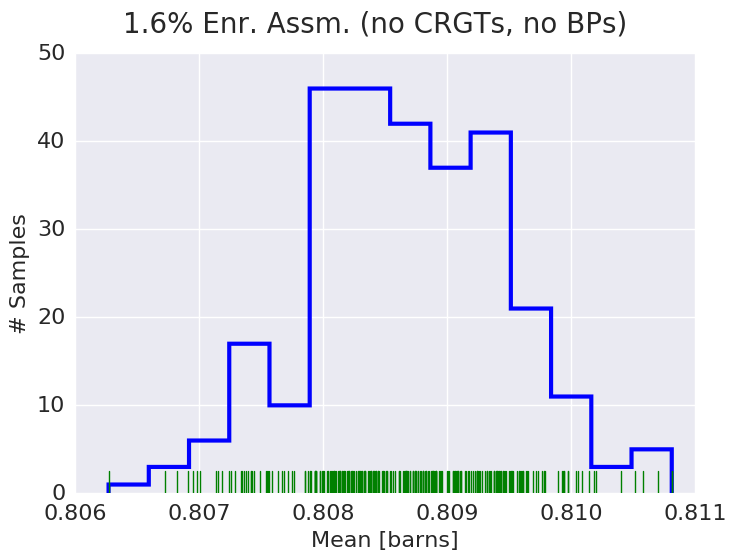
\includegraphics[width=\linewidth]{figures/patterns/assm-1.6-inf/hist-kde-rug/assm-16-inf-capt-1}
  \caption{}
  \label{fig:chap9-hist-assm-1.6-inf-capt}
\end{subfigure}%
\begin{subfigure}{0.5\textwidth}
  \centering
  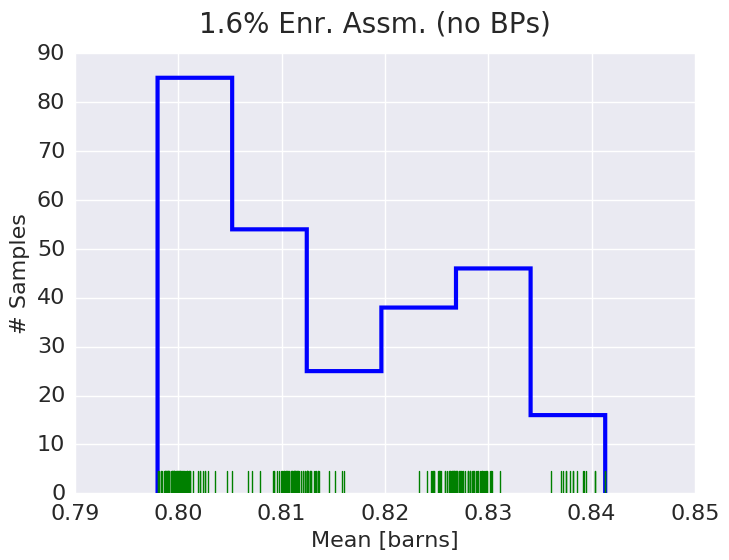
\includegraphics[width=\linewidth]{figures/patterns/assm-1.6/hist-kde-rug/assm-16-capt-1}
  \caption{}
  \label{fig:chap9-hist-assm-1.6-capt}
\end{subfigure}
\begin{subfigure}{0.5\textwidth}
  \centering
  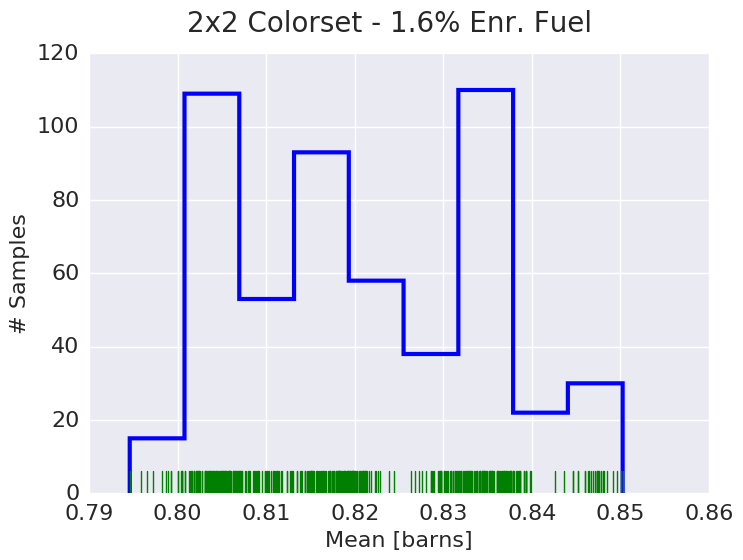
\includegraphics[width=\linewidth]{figures/patterns/2x2/hist-kde-rug/16-enr-capt-1}
  \caption{}
  \label{fig:chap9-hist-2x2-1.6-capt}
\end{subfigure}%
\begin{subfigure}{0.5\textwidth}
  \centering
  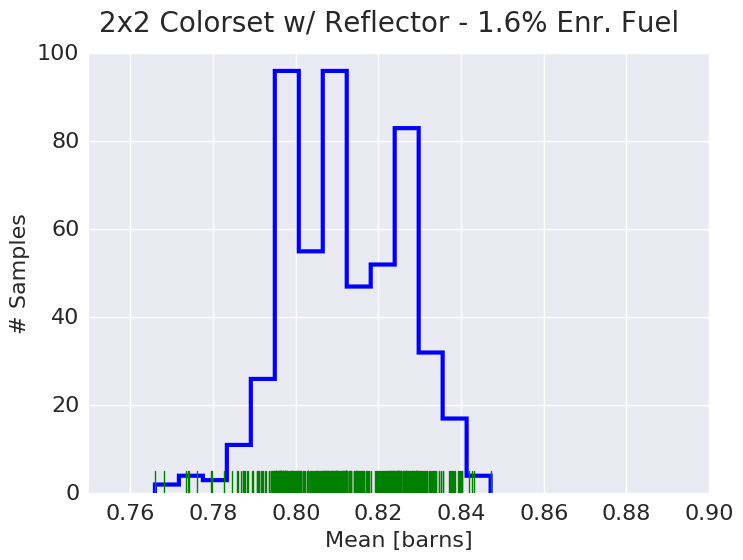
\includegraphics[width=\linewidth]{figures/patterns/reflector/hist-kde-rug/16-enr-capt-1}  \caption{}
  \label{fig:chap9-hist-reflector-1.6-capt}
\end{subfigure}
\begin{subfigure}{0.5\textwidth}
  \centering
  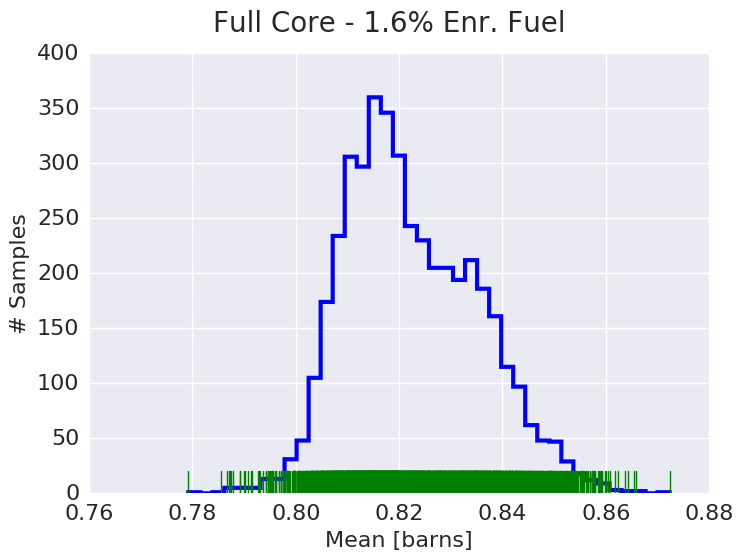
\includegraphics[width=\linewidth]{figures/patterns/full-core/hist-kde-rug/16-enr-capt-1} \caption{}
  \label{fig:chap9-hist-full-core-1.6-capt}
\end{subfigure}
\caption[Histogram of U-238 capture MGXS for 1.6\% enriched fuel]{Histograms of U-238 capture \ac{MGXS} (group 1 of 2) for 1.6\% enriched fuel.}
\label{fig:chap9-hist-1.6-capt}
\end{figure}

\begin{figure}[h!]
\centering
\begin{subfigure}{0.5\textwidth}
  \centering
  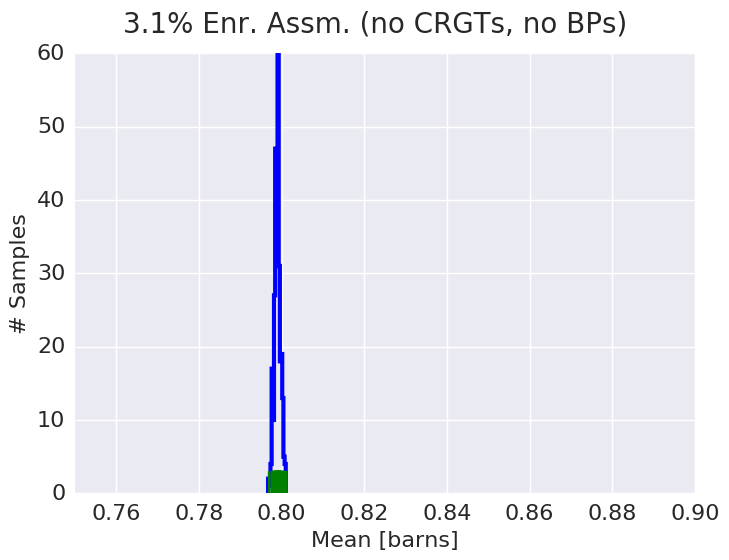
\includegraphics[width=\linewidth]{figures/patterns/assm-3.1-inf/hist-kde-rug/assm-31-inf-capt-1}
  \caption{}
  \label{fig:chap9-hist-assm-3.1-inf-capt}
\end{subfigure}%
\begin{subfigure}{0.5\textwidth}
  \centering
  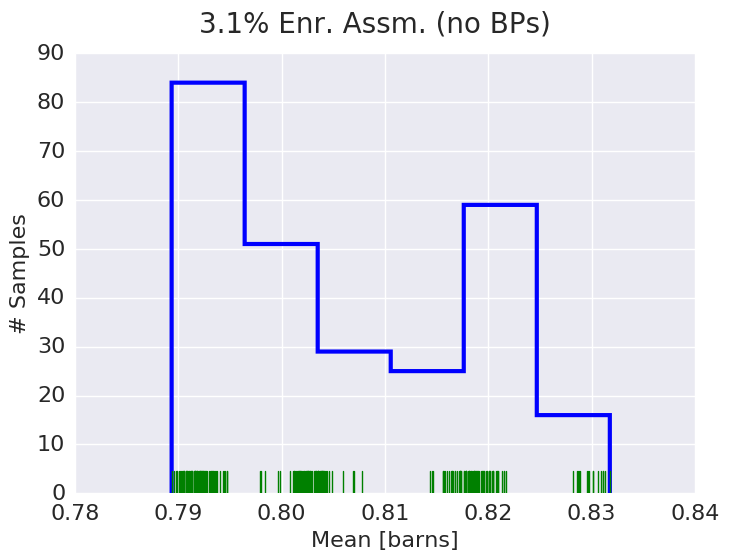
\includegraphics[width=\linewidth]{figures/patterns/assm-3.1/hist-kde-rug/assm-31-capt-1}
  \caption{}
  \label{fig:chap9-hist-assm-3.1-capt}
\end{subfigure}
\begin{subfigure}{0.5\textwidth}
  \centering
  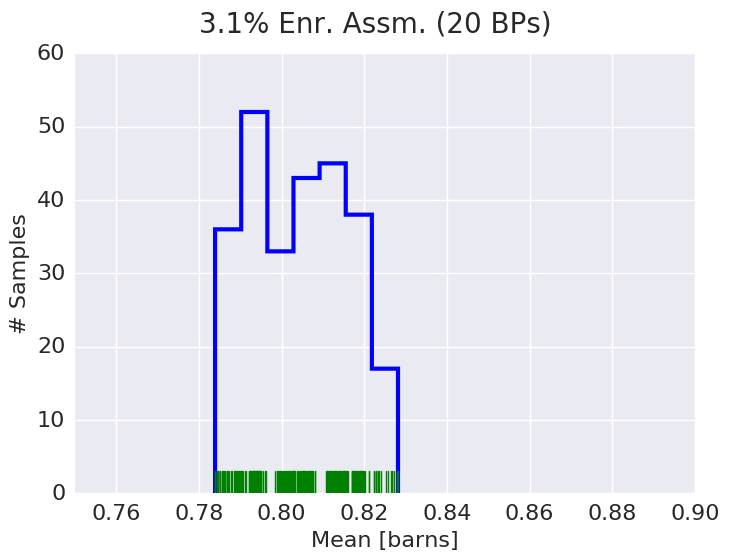
\includegraphics[width=\linewidth]{figures/patterns/assm-3.1-20BPs/hist-kde-rug/assm-31-20BPs-capt-1}
  \caption{}
  \label{fig:chap9-hist-assm-3.1-20BPs-capt}
\end{subfigure}%
\begin{subfigure}{0.5\textwidth}
  \centering
  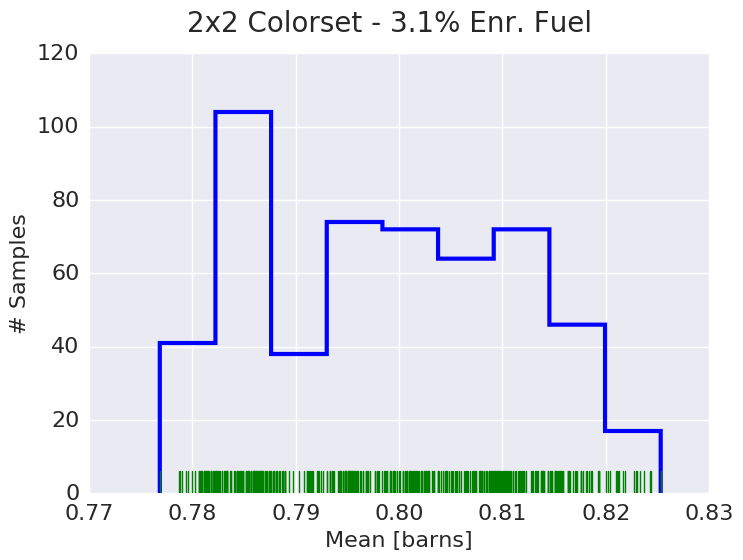
\includegraphics[width=\linewidth]{figures/patterns/2x2/hist-kde-rug/31-enr-capt-1}
  \caption{}
  \label{fig:chap9-hist-2x2-3.1-capt}
\end{subfigure}
\begin{subfigure}{0.5\textwidth}
  \centering
  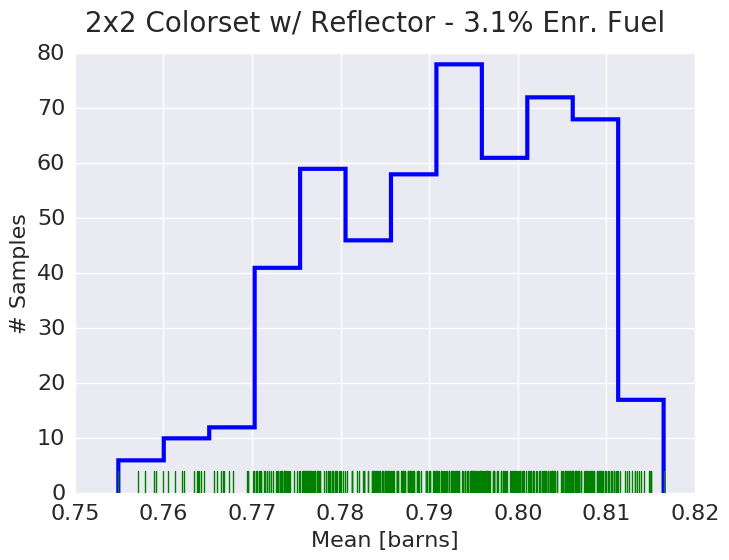
\includegraphics[width=\linewidth]{figures/patterns/reflector/hist-kde-rug/31-enr-capt-1}  \caption{}
  \label{fig:chap9-hist-reflector-3.1-capt}
\end{subfigure}%
\begin{subfigure}{0.5\textwidth}
  \centering
  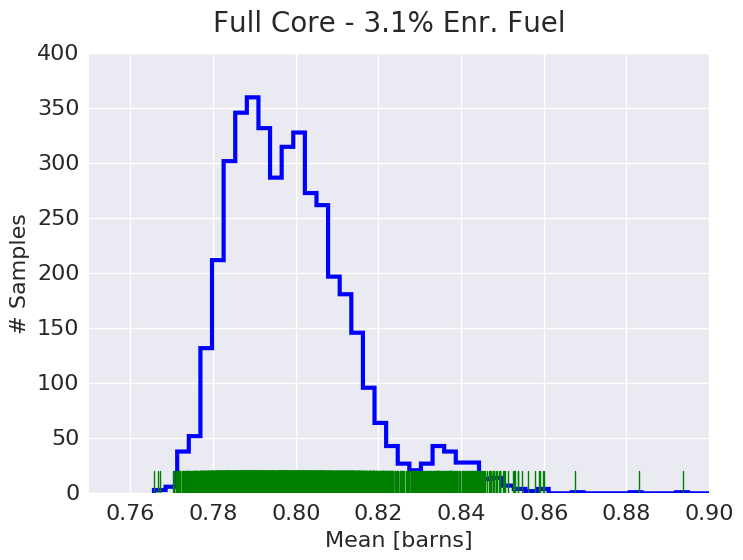
\includegraphics[width=\linewidth]{figures/patterns/full-core/hist-kde-rug/31-enr-capt-1} \caption{}
  \label{fig:chap9-hist-full-core-3.1-capt}
\end{subfigure}
\caption[Histogram of U-238 capture MGXS for 3.1\% enriched fuel]{Histograms of U-238 capture \ac{MGXS} (group 1 of 2) for 3.1\% enriched fuel.}
\label{fig:chap9-hist-3.1-capt}
\end{figure}

The inter-assembly interfaces in the 2$\times$2 colorset benchmark results in a further ``smearing'' of the clusters for both enrichments in Figs.~\ref{fig:chap9-hist-2x2-1.6-capt} and~\ref{fig:chap9-hist-2x2-3.1-capt}. It should be noted that there are twice as many samples (\textit{e.g.}, 528 fuel pin instances for each enrichment) in the colorsets than the individual fuel assemblies. Hence, it is more challenging to distinguish clusters from the rug plots for the larger colorset benchmarks. Nonetheless, the histograms indicate the continuing presence of four distinct clusters for both enrichments, though they are easier to identify for the 1.6\% enriched fuel pins (in assemblies without \acp{BP}). The \ac{MGXS} are generally shifted up by $\sim$0.01 barns for the 1.6\% enriched pins, and down by $\sim$0.0075 barns for the 3.1\% enriched pins, with respect to the individual fuel assemblies.

The introduction of a reflector to the 2$\times$2 colorset leads to very different distributions for the two fuel enrichments in Figs.~\ref{fig:chap9-hist-reflector-1.6-capt} and~\ref{fig:chap9-hist-reflector-3.1-capt}. The reason for this is that periodicity along the $x$ and $y$ axes is broken with the inclusion of the reflector. In particular, both of the 3.1\% enriched assemblies are symmetrically adjacent to the reflector, and therefore have identical pin-wise \ac{MGXS}. However, one of the 1.6\% enriched assemblies is corner adjacent to the reflector while the other is located within the interior of the colorset. Nevertheless, some general observations can be made from the data. First, the \ac{MGXS} are generally even more ``smeared'' for both enrichments than is the case for the colorset without a reflector. The histogram indicates the existence of at least three clusters for the 1.6\% enriched pins, with a similar but less concentrated three-way clustering for the 3.1\% enriched pins. Finally, the lowest pin-wise \ac{MGXS} for both enrichments are $\sim$0.025 barns (or $\sim$3\%) less than those in the colorset without a reflector. This may be due to a harder spectrum in fuel pins along the left and top boundaries which have periodic \acp{BC} in the colorset without a reflector, but reflective \acp{BC} for the colorset with a water reflector.

%-trends w/ reflector
%  -pins with smallest \ac{MGXS} shifted down by $\sim$0.025 barns
%  -perhaps the uncertainties are just larger for the reflector and those pins are outliers??

The quarter core \ac{BEAVRS} model has the smoothest varying distributions of any of the benchmarks in Figs.~\ref{fig:chap9-hist-full-core-1.6-capt} and~\ref{fig:chap9-hist-full-core-3.1-capt}. This is due in part to the fact that there are over 8$\times$ more samples for each fuel enrichment than are present for the colorsets\footnote{There are 4,332 1.6\%, 4,260 2.4\% and 4,236 3.1\% enriched fuel pins in the quarter core model.}. The most notable observation is that the distributions appear to first order to be bimodal with large peaks centered at approximately 0.815 and 0.83 barns, and 0.785 and 0.805 barns, for the 1.6\% and 3.1\% enriched pins, respectively. The distribution for the 3.1\% enriched fuel pins has an additional smaller shoulder centered at 0.83 barns. Additionally, a few 3.1\% enriched pins have significantly greater \ac{MGXS} between 0.86 and 0.9 barns. This is likely due to the fact that the 3.1\% enriched assemblies surround the exterior of the core configuration. As a result, the flux is more strongly shielded in the U-238 resonance energies for 3.1\% enriched pins adjacent to the baffle/reflector than the 1.6\% enriched pins in the interior, resulting in some larger ``outlier'' pin-wise \ac{MGXS}.

Finally, it should be noted that the microscopic U-238 capture \ac{MGXS} are generally 0.01 -- 0.02 barns (or 1.25 -- 2.5\%) larger for the 1.6\% than the 3.1\% enriched fuel pins for each respective benchmark, including the infinite lattice. These results indicate that the flux is less shielded at resonance energies for the lesser enriched fuel, perhaps due to a slightly larger fraction of neutrons up-scattering from group two to one due to the smaller probability of fission. This variation of U-238 capture \ac{MGXS} with fuel enrichment remains true even for the quarter core \ac{BEAVRS} model. However, the single largest U-238 capture \ac{MGXS} is in a 3.1\% enriched fuel pin corner adjacent to the baffle, which likely has the softest spectrum of any pin due to the nearby reflector.

%due to its lower dilution cross section

%This is counter-intuitive to what one might expect -- namely, that the removal of neutrons in U-238 capture resonances would shield the flux in energy intervals where the U-238 capture cross section is greatest, reducing the flux-weighted energy-integrated \ac{MGXS}. However, 

%This may be due to a more strongly peaked ``rim effect'' of U-238 capture along the pin-moderator interface in the 1.6\% enriched pins. As a result, the flux at the interior of the lesser enriched pins may be less shielded  at resonance energies, leading to a slightly larger 

%This effect is likely due to the removal of neutrons in U-238 capture resonances as they traverse each fuel pin. As a result, the flux in those energy intervals where the U-238 capture cross section is greatest and hence reducing the flux-weighted energy-integrated \ac{MGXS}. Interestingly, this impact  

\begin{emphbox}
\textbf{The dispersion of pin-wise U-238 capture \ac{MGXS} is highly uneven and structured. Core heterogeneities such as \acp{CRGT}, \acp{BP} and reflectors induce clustering due to spatial self-shielding effects which are observed from distributions of the pin-wise \ac{MGXS}.}
\end{emphbox}

%%%%%%%%%%%%%%%%%%%%%%%%%%%%%%%%%%
\subsubsection{U-235 Fission MGXS}
\label{subsubsec:chap9-histograms-fiss}

The pin-wise microscopic U-235 fission \ac{MGXS} for 1.6\% and 3.1\% enriched fuel pins are illustrated with histograms and rug plots in Figs.~\ref{fig:chap9-hist-1.6-fiss} and~\ref{fig:chap9-hist-3.1-fiss}, respectively. It should first be noted that the U-235 fission \ac{MGXS} are over 300$\times$ larger than the U-238 capture \ac{MGXS} illustrated in the preceding section. However, it should be recalled that the U-238 nuclide density is over 30 -- 60$\times$ larger than U-235 in the 1.6\% and 3.1\% enriched fuel, respectively. As a consequence, the clustering of either microscopic U-238 capture or the U-235 fission \ac{MGXS} is important since it will have a similarly sized impact on the corresponding macroscopic \ac{MGXS} and reaction rates.

\begin{figure}[h!]
\centering
\begin{subfigure}{0.5\textwidth}
  \centering
  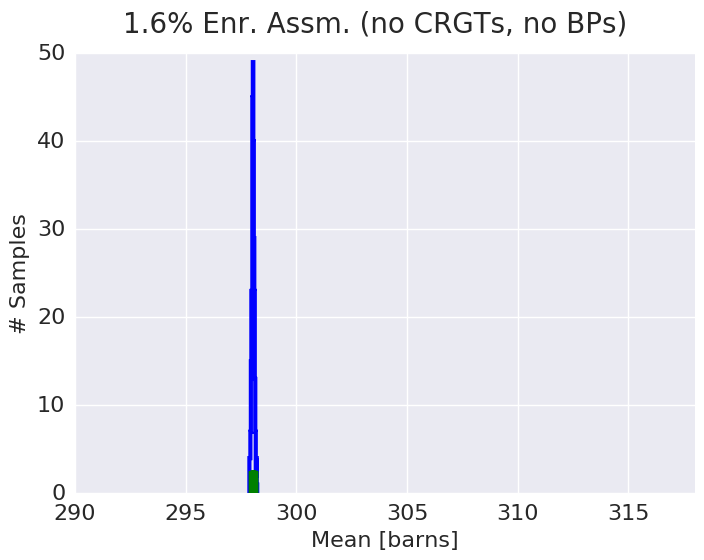
\includegraphics[width=\linewidth]{figures/patterns/assm-1.6-inf/hist-kde-rug/assm-16-inf-fiss-2}
  \caption{}
  \label{fig:chap9-hist-assm-1.6-inf-fiss}
\end{subfigure}%
\begin{subfigure}{0.5\textwidth}
  \centering
  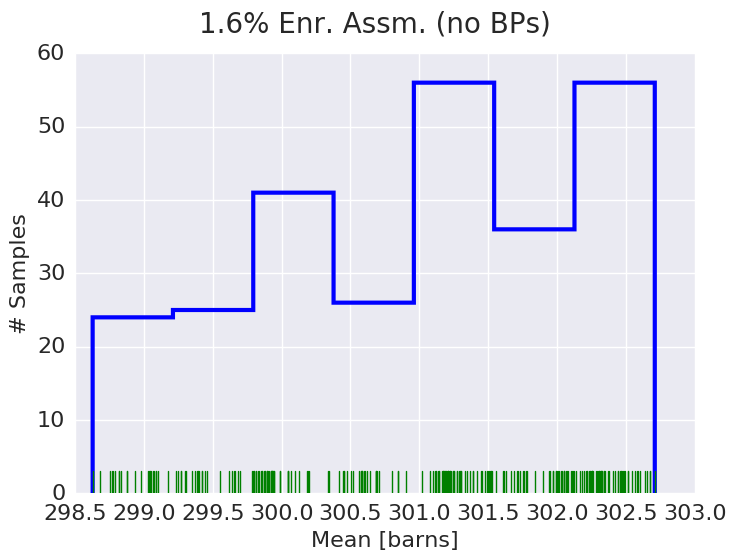
\includegraphics[width=\linewidth]{figures/patterns/assm-1.6/hist-kde-rug/assm-16-fiss-2}
  \caption{}
  \label{fig:chap9-hist-assm-1.6-fiss}
\end{subfigure}
\begin{subfigure}{0.5\textwidth}
  \centering
  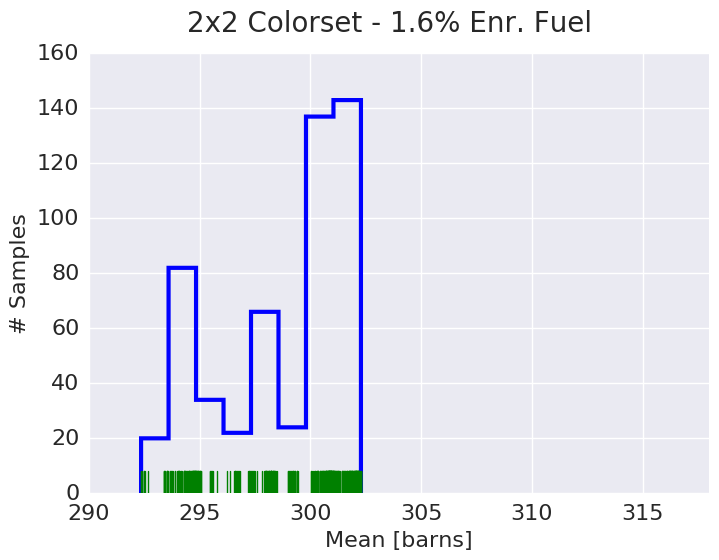
\includegraphics[width=\linewidth]{figures/patterns/2x2/hist-kde-rug/16-enr-fiss-2}
  \caption{}
  \label{fig:chap9-hist-2x2-1.6-fiss}
\end{subfigure}%
\begin{subfigure}{0.5\textwidth}
  \centering
  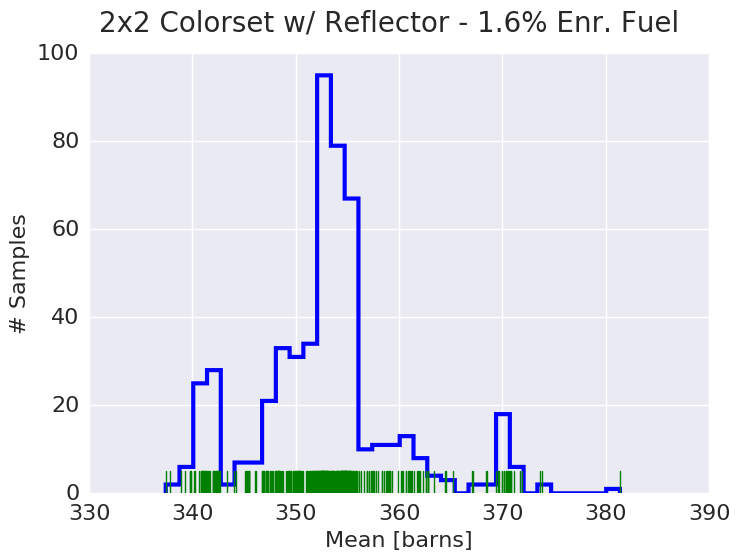
\includegraphics[width=\linewidth]{figures/patterns/reflector/hist-kde-rug/16-enr-fiss-2}  \caption{}
  \label{fig:chap9-hist-reflector-1.6-fiss}
\end{subfigure}
\begin{subfigure}{0.5\textwidth}
  \centering
  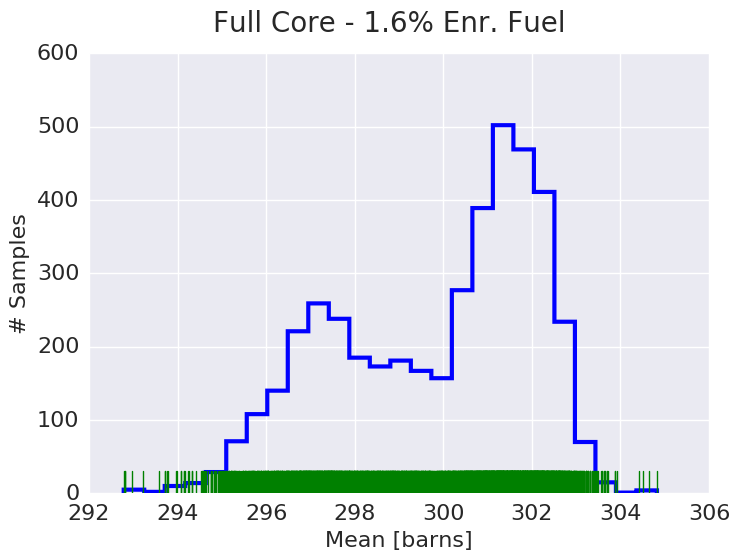
\includegraphics[width=\linewidth]{figures/patterns/full-core/hist-kde-rug/16-enr-fiss-2} \caption{}
  \label{fig:chap9-hist-full-core-1.6-fiss}
\end{subfigure}
\caption[Histogram of U-235 fission MGXS for 1.6\% enriched fuel]{Histograms of U-235 fission \ac{MGXS} (group 2 of 2) for 1.6\% enriched fuel.}
\label{fig:chap9-hist-1.6-fiss}
\end{figure}

\begin{figure}[h!]
\centering
\begin{subfigure}{0.5\textwidth}
  \centering
  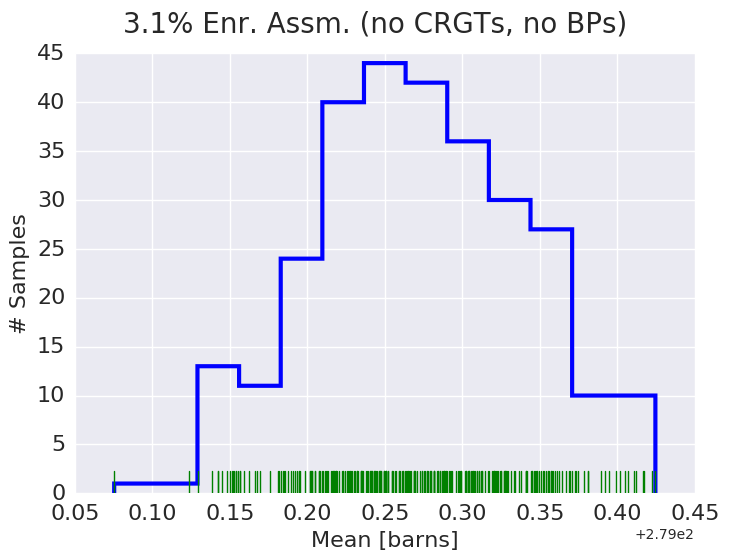
\includegraphics[width=\linewidth]{figures/patterns/assm-3.1-inf/hist-kde-rug/assm-31-inf-fiss-2}
  \caption{}
  \label{fig:chap9-hist-assm-3.1-inf-fiss}
\end{subfigure}%
\begin{subfigure}{0.5\textwidth}
  \centering
  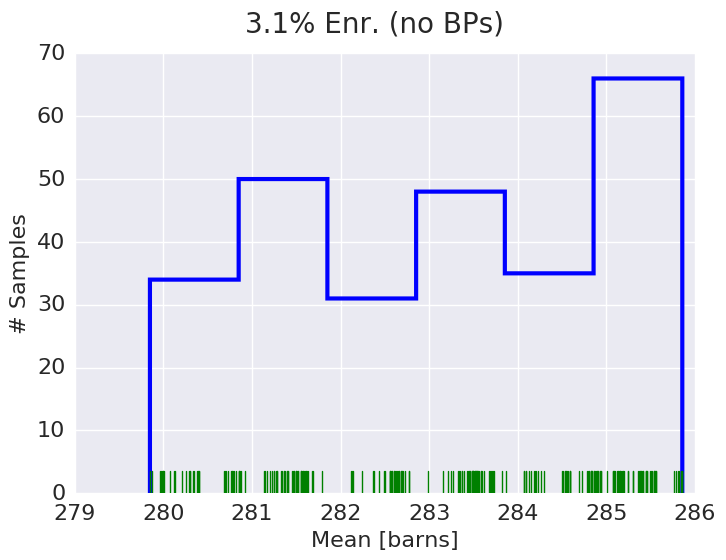
\includegraphics[width=\linewidth]{figures/patterns/assm-3.1/hist-kde-rug/assm-31-fiss-2}
  \caption{}
  \label{fig:chap9-hist-assm-3.1-fiss}
\end{subfigure}
\begin{subfigure}{0.5\textwidth}
  \centering
  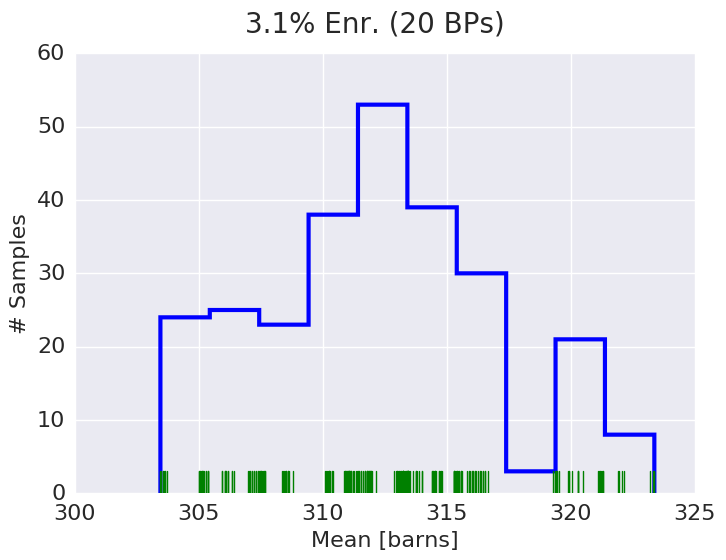
\includegraphics[width=\linewidth]{figures/patterns/assm-3.1-20BPs/hist-kde-rug/assm-31-20BPs-fiss-2}
  \caption{}
  \label{fig:chap9-hist-assm-3.1-20BPs-fiss}
\end{subfigure}%
\begin{subfigure}{0.5\textwidth}
  \centering
  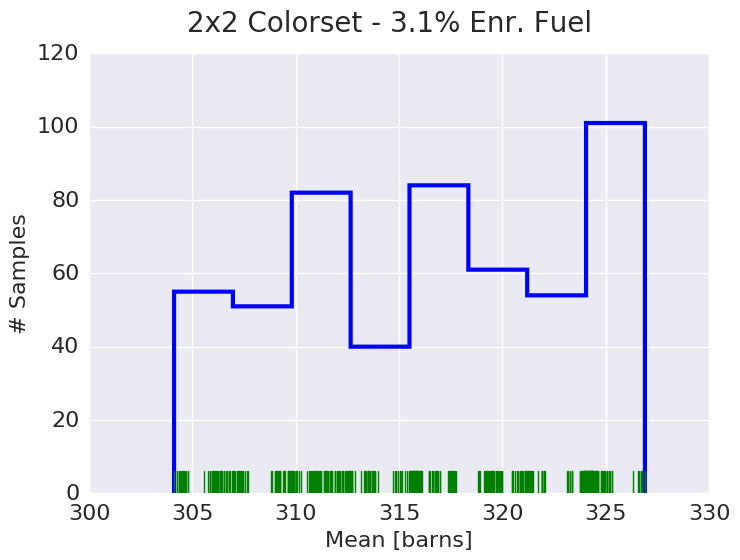
\includegraphics[width=\linewidth]{figures/patterns/2x2/hist-kde-rug/31-enr-fiss-2}
  \caption{}
  \label{fig:chap9-hist-2x2-3.1-fiss}
\end{subfigure}
\begin{subfigure}{0.5\textwidth}
  \centering
  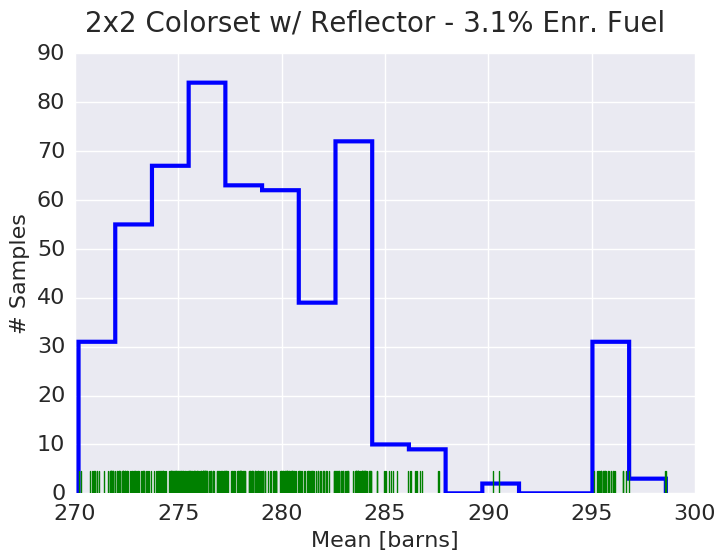
\includegraphics[width=\linewidth]{figures/patterns/reflector/hist-kde-rug/31-enr-fiss-2}  \caption{}
  \label{fig:chap9-hist-reflector-3.1-fiss}
\end{subfigure}%
\begin{subfigure}{0.5\textwidth}
  \centering
  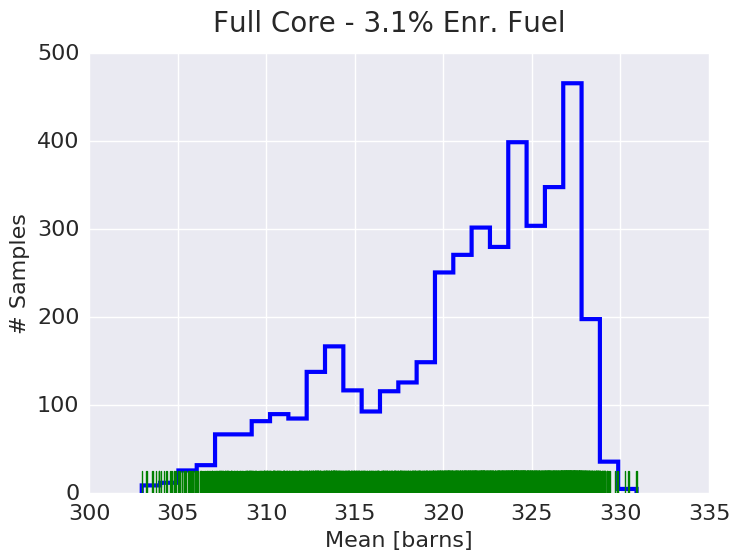
\includegraphics[width=\linewidth]{figures/patterns/full-core/hist-kde-rug/31-enr-fiss-2} \caption{}
  \label{fig:chap9-hist-full-core-3.1-fiss}
\end{subfigure}
\caption[Histogram of U-235 fission MGXS 3.1\% enriched fuel]{Histograms of U-235 fission \ac{MGXS} (group 2 of 2) for 3.1\% enriched fuel.}
\label{fig:chap9-hist-3.1-fiss}
\end{figure}

As was observed for U-238 capture, the distributions of pin-wise \ac{MGXS} for the infinite lattices in Figs.~\ref{fig:chap9-hist-assm-1.6-inf-fiss} and~\ref{fig:chap9-hist-assm-3.1-inf-fiss} are narrow and symmetric unlike the distributions for each of the heterogeneous benchmarks. Unlike the situation for U-238 capture, the introduction of \acp{CRGT} induces a more intricate clustering of the U-235 fission \ac{MGXS} in Figs.~\ref{fig:chap9-hist-assm-1.6-fiss} and~\ref{fig:chap9-hist-assm-3.1-fiss}. However, the total range of U-235 fission \ac{MGXS} in the fuel assemblies with \acp{CRGT} varies by only 1 -- 2\% as compared to more than 5\% for U-238 capture. The histograms indicate the presence of roughly three clusters of \ac{MGXS} which are separated by 1 -- 2 barns for both fuel enrichments. The rug plots illustrate a more complicated dispersion, however, with a significantly more distinct concentration into approximately eight clusters for the 3.1\% enriched fuel pins. These observations indicate that U-235 fission may be more sensitive than U-238 capture to spatial self-shielding effects from the added moderation of \acp{CRGT}, even though the impact on the resultant \ac{MGXS} is of a smaller relative magnitude. This is the result of the $\nicefrac{1}{v}$ profile of the U-235 fission cross section at thermal energies which is particularly sensitive to thermalization when weighted by the flux to compute \ac{MGXS}.

The further addition of \acp{BP} to the 3.1\% enriched fuel assembly results in a more distinct set of isolated clusters of U-235 fission \ac{MGXS} in Fig.~\ref{fig:chap9-hist-assm-3.1-20BPs-fiss}. In particular, there appear to be three overall clusters centered at approximately 272, 276 and 300 barns each with a number of sub-clusters. This stands in contrast to the case for U-238 capture where the presence of \acp{BP} resulted in a ``smearing'' of the clusters. In addition, the \ac{MGXS} are generally shifted downwards by 5 -- 10  barns (or 1.5 -- 3\%) with respect to the assembly without \acp{BP}. The inter-assembly interfaces in the 2$\times$2 colorset benchmark have a similarly concentrating effect for both enrichments in Figs.~\ref{fig:chap9-hist-2x2-1.6-fiss} and~\ref{fig:chap9-hist-2x2-3.1-fiss}. The histograms reveal three clusters centered at approximately 294, 298 and 301 barns for the 1.6\% enriched pins, and four clusters centered at 271, 275, 278 and 283 barns for the 3.1\% enriched pins. Furthermore, the rug plots indicate the presence of more clusters which are easier to distinguish than they are for the individual fuel assemblies, or for the U-238 capture \ac{MGXS} in the 2$\times$2 colorset benchmark. Finally, the \ac{MGXS} in the colorset are generally shifted downwards by 3 -- 6  barns (or 1 -- 2\%) with respect to the individual fuel assemblies.

The introduction of a reflector to the 2$\times$2 colorset leads to very different distributions for the two fuel enrichments in Figs.~\ref{fig:chap9-hist-reflector-1.6-fiss} and~\ref{fig:chap9-hist-reflector-3.1-fiss}. As was noted in Sec.~\ref{subsubsec:chap9-histograms-capt}, the reason for this is that symmetry is broken with the inclusion of the reflector. A first observation is that the distributions of U-235 fission \ac{MGXS} for the two enrichments differ much more profoundly than they do for U-238 capture. The histogram for the 1.6\% enriched pins indicate perhaps six primary clusters centered at 294, 298, 301, 304, 306 and 310 barns, though the rug plot certainly indicates the presence of even more sub-clusters. The histogram for the 3.1\% enriched pins indicate perhaps four clusters roughly centered at 276, 284, 290 and 296 barns, though the intervals between these apparent clusters contain many additional samples, complicating the analysis. Finally, the largest U-235 fission \ac{MGXS} are approximately 315 and 300 barns for the 1.6\% and 3.1\% enriched pins in the colorset, respectively, about 15 barns (or 5\%) greater than the largest \ac{MGXS} for the colorset without a reflector. This is due to the softer flux spectrum experienced by those pins adjacent to the reflector.

As was noted for the U-238 capture \ac{MGXS}, the quarter core \ac{BEAVRS} model has the smoothest varying distributions of any of the benchmarks in Figs.~\ref{fig:chap9-hist-full-core-1.6-fiss} and~\ref{fig:chap9-hist-full-core-3.1-fiss}. The most notable observation is that the distributions appear to first order to be bimodal and trimodal with large peaks centered at approximately 297 and 302 barns, and 278, 283 and 284 barns, for the 1.6\% and 3.1\% enriched pins, respectively. The two peaks are more clearly discernible for the 1.6\% enriched fuel pins. This effect may be due to an increase in moderation for those 1.6\% enriched assemblies that are only one assembly removed from the reflector as compared to those in the interior of the core. Furthermore, the range of \ac{MGXS} in the quarter core model only spans 10 -- 15 barns (or 5\%) as compared to the 20 -- 25 barns for the 2$\times$ colorset benchmark. This is likely due to the presence of a stainless steel baffle separating the assemblies on the exterior of the \ac{BEAVRS} model from the water reflector. The baffle dampens the additional moderation experienced by those pins nearest the reflector in the \ac{BEAVRS} model with respect to those in the 2$\times$2 colorset with a reflector but no baffle.

Finally, it should be noted that the microscopic U-235 fission \ac{MGXS} are generally 18 -- 22 barns (or 6+\%) larger for the 1.6\% than the 3.1\% enriched fuel pins for each respective benchmark, including the infinite lattice. These results indicate that the flux is more strongly moderated for the lesser enriched fuel, perhaps due to the smaller probability of fission. This variation of U-235 fission \ac{MGXS} with fuel enrichment remains true even for the quarter core \ac{BEAVRS} model. 

\begin{emphbox}
\textbf{The presence of core heterogeneities induce more clearly defined clustering of pin-wise U-235 fission \ac{MGXS} than is observed for U-238 capture (in 2-group data). However, the population of pin-wise U-235 fission \ac{MGXS} only vary by up to 1\% about the mean, while the U-238 capture \ac{MGXS} variation is $\sim$2.5\%.}
\end{emphbox}

%%%%%%%%%%%%%%%%%%%%%%%%%%%%%%%%%%%%%%%%%%%%%%%%%%%%%
\subsection{Quantile-Quantile Plots of Pin-Wise MGXS}
\label{subsec:chap9-qq-plots}

This section illustrates the deviation from normality of pin-wise \ac{MGXS} with \ac{Q-Q} plots. A \ac{Q-Q} plot is used to compare two datasets drawn from different probability distributions. In particular, the quantiles from one dataset are plotted against the quantiles of a second dataset in an $(x,y)$ scatter plot\footnote{A \textit{quantile} is the point at which some fraction of the data falls below a given value. For example, the 10\% quantile is the point at which 10\% of the data is below the point and 90\% is above it.}. If the two distributions are similar, the data points will lie along the $y = x$ reference line. Departures from $y = x$ indicate dis-similarities between the distributions, such as shifts in location or scale, changes in symmetry, and outliers. 

\interfootnotelinepenalty=10000

In this section, the theoretical quantiles for a normal distribution are plotted against empirical quantiles found from the empirical distribution of pin-wise U-238 capture and U-235 fission \ac{MGXS}. These \ac{Q-Q} plots illustrate the deviation from normality for the data as heterogeneities are introduced to the benchmark models. It should be noted that the \ac{MGXS} data is first standardized so that it can be compared to theoretical quantiles from a standard normal distribution $\mathcal{N}(0,1)$ in the \ac{Q-Q} plots. The visualizations are presented for an infinite lattice as well as the six heterogeneous benchmarks for both 1.6\% and 3.1\% enriched fuel. The random samples in each visualization (\textit{e.g.}, each blue data point) correspond to a single fuel pin instance in the corresponding benchmark model. In addition, each plot highlights the $p$-value\footnote{The $p$-value is used in null hypothesis significance testing and measures the likelihood of an observation as or more extreme than the given one. In this section, the null hypothesis is that pin-wise \ac{MGXS} data is drawn from a normal distribution. To test this hypothesis, a significance level $\alpha$ is chosen (\textit{e.g.}, 1\%) and compared with the $p$-value of the Shapiro-Wilk normality test. If $p < \alpha$ then the null hypothesis is rejected (\textit{i.e.}, the dataset was not drawn from a normal distribution); otherwise, it cannot be rejected.} for the Shapiro-Wilk test of normality~\cite{shapiro1965analysis} computed using the Python \texttt{scipy.stats} package~\cite{jones2011scipy}\footnote{The implementation of the Shapiro-Wilk test in \texttt{scipy.stats} is stated to be accurate up to at least 5,000 data points. This is suitable for the datasets considered here which are largest for the quarter core \ac{BEAVRS} model with $\sim$4,500 points for the each fuel enrichment.}.

%%%%%%%%%%%%%%%%%%%%%%%%%%%%%%%%%%
\subsubsection{U-238 Capture MGXS}
\label{subsubsec:chap9-qq-plots-capt}

The pin-wise microscopic U-238 capture \ac{MGXS} for 1.6\% and 3.1\% enriched fuel pins are illustrated with histograms and rug plots in Fig.~\ref{fig:chap9-qq-1.6-capt} and~\ref{fig:chap9-qq-3.1-capt}, respectively. As was hypothesized earlier, the datasets for the infinite lattices in Figs.~\ref{fig:chap9-qq-assm-1.6-inf-capt} and~\ref{fig:chap9-qq-assm-3.1-inf-capt} appear to be from a normal distribution since they lie very close to the $y = x$ reference line. In addition, the $p$-values are greater than 0.7, well above commonly used significance levels; thus one would not reject the null hypothesis that the data is from a normal distribution. The addition of \acp{CRGT} leads to a clear deviation from normality in Figs.~\ref{fig:chap9-qq-assm-1.6-capt} and~\ref{fig:chap9-qq-assm-3.1-capt}, with four ``shoulders'' representing the four clusters highlighted in Sec.~\ref{subsec:chap9-histograms} for the single assembly benchmarks. The presence of \acp{BP} seems to result in more shoulders in Fig.~\ref{fig:chap9-qq-assm-3.1-20BPs-capt} corresponding to the various clusters identified in Fig.~\ref{fig:chap9-hist-assm-3.1-20BPs-capt}. 

\begin{figure}[h!]
\centering
\begin{subfigure}{0.5\textwidth}
  \centering
  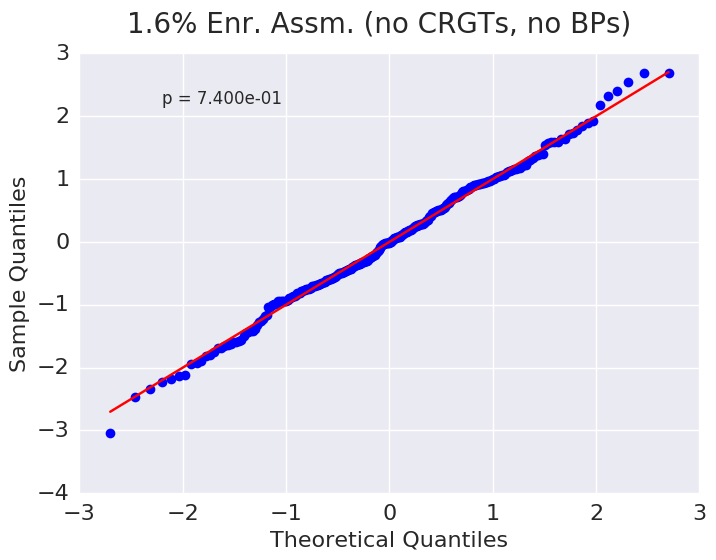
\includegraphics[width=\linewidth]{figures/patterns/assm-1.6-inf/quantile/assm-16-inf-capt-1}
  \caption{}
  \label{fig:chap9-qq-assm-1.6-inf-capt}
\end{subfigure}%
\begin{subfigure}{0.5\textwidth}
  \centering
  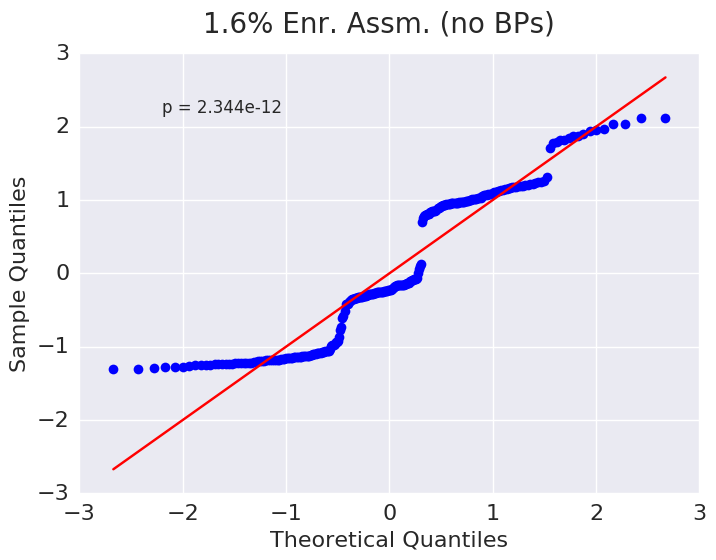
\includegraphics[width=\linewidth]{figures/patterns/assm-1.6/quantile/assm-16-capt-1}
  \caption{}
  \label{fig:chap9-qq-assm-1.6-capt}
\end{subfigure}
\begin{subfigure}{0.5\textwidth}
  \centering
  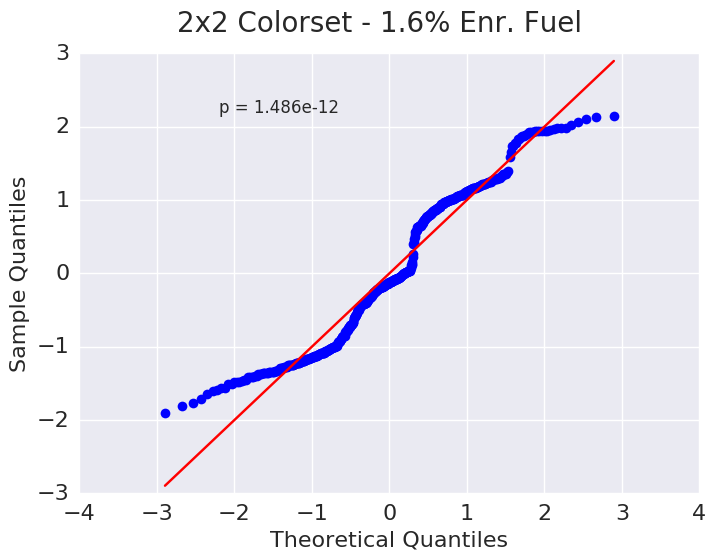
\includegraphics[width=\linewidth]{figures/patterns/2x2/quantile/16-enr-capt-1}
  \caption{}
  \label{fig:chap9-qq-2x2-1.6-capt}
\end{subfigure}%
\begin{subfigure}{0.5\textwidth}
  \centering
  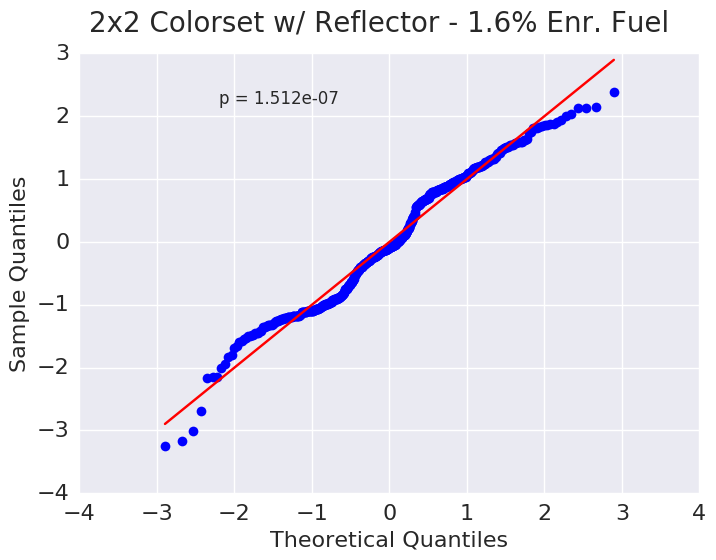
\includegraphics[width=\linewidth]{figures/patterns/reflector/quantile/16-enr-capt-1}  \caption{}
  \label{fig:chap9-qq-reflector-1.6-capt}
\end{subfigure}
\begin{subfigure}{0.5\textwidth}
  \centering
  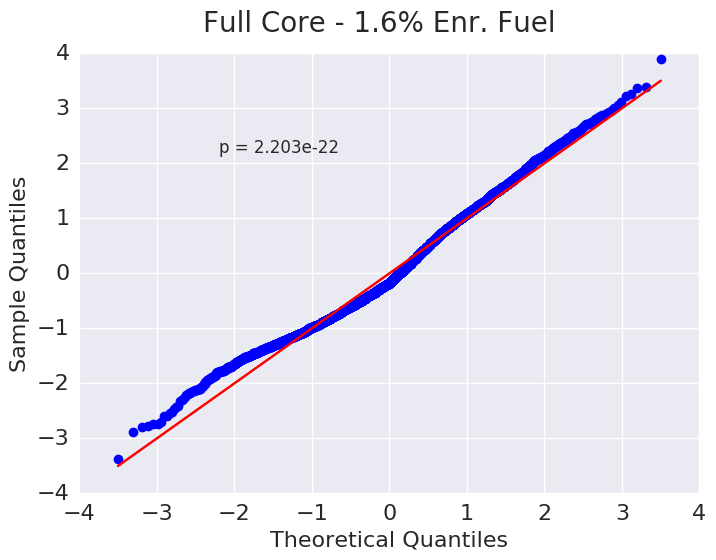
\includegraphics[width=\linewidth]{figures/patterns/full-core/quantile/16-enr-capt-1} \caption{}
  \label{fig:chap9-qq-full-core-1.6-capt}
\end{subfigure}
\caption[Q-Q plots of U-238 capture MGXS for 1.6\% enriched fuel]{\ac{Q-Q} plots of U-238 capture \ac{MGXS} (group 1 of 2) for 1.6\% enriched fuel.}
\label{fig:chap9-qq-1.6-capt}
\end{figure}

\begin{figure}[h!]
\centering
\begin{subfigure}{0.5\textwidth}
  \centering
  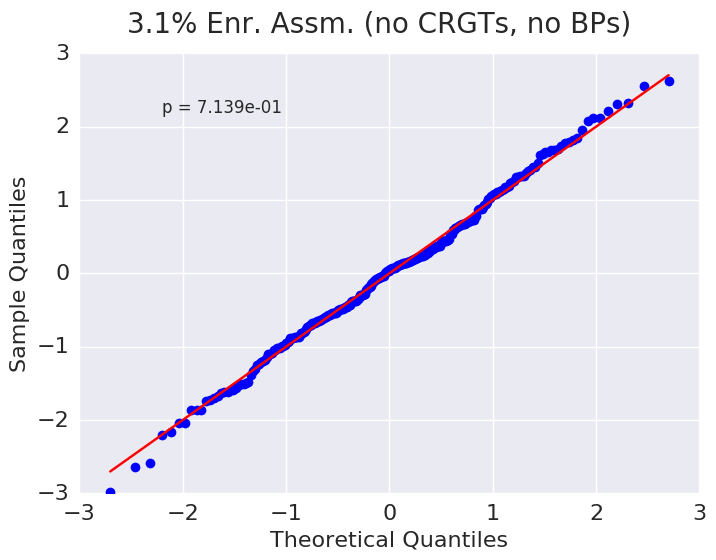
\includegraphics[width=\linewidth]{figures/patterns/assm-3.1-inf/quantile/assm-31-inf-capt-1}
  \caption{}
  \label{fig:chap9-qq-assm-3.1-inf-capt}
\end{subfigure}%
\begin{subfigure}{0.5\textwidth}
  \centering
  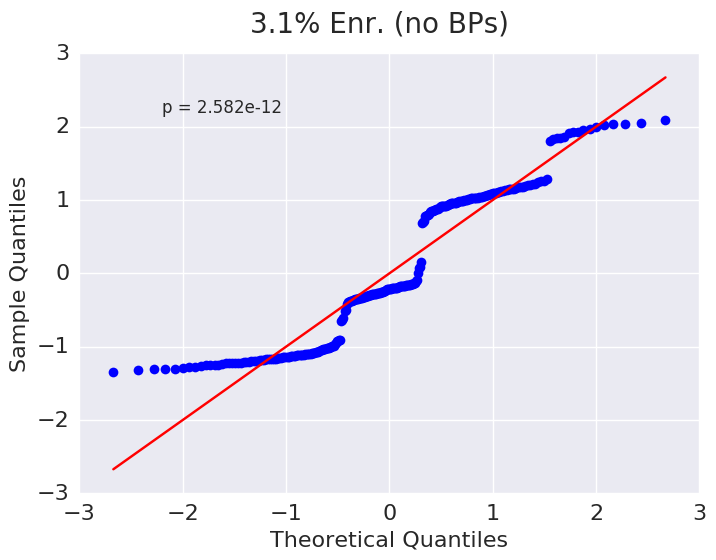
\includegraphics[width=\linewidth]{figures/patterns/assm-3.1/quantile/assm-31-capt-1}
  \caption{}
  \label{fig:chap9-qq-assm-3.1-capt}
\end{subfigure}
\begin{subfigure}{0.5\textwidth}
  \centering
  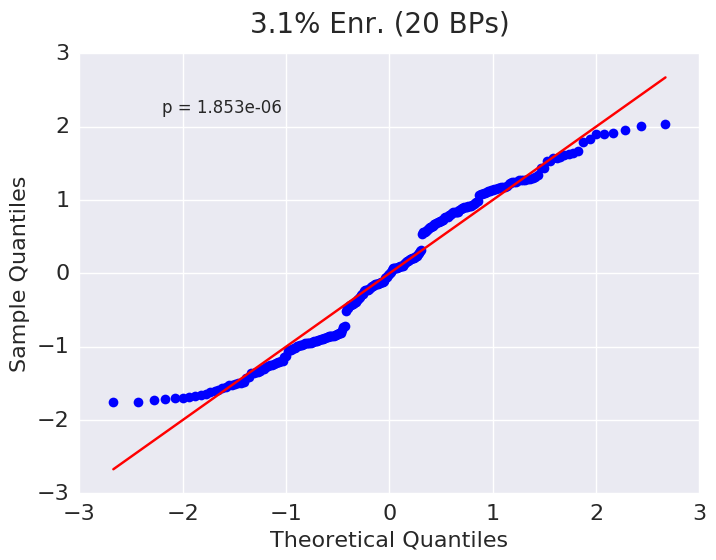
\includegraphics[width=\linewidth]{figures/patterns/assm-3.1-20BPs/quantile/assm-31-20BPs-capt-1}
  \caption{}
  \label{fig:chap9-qq-assm-3.1-20BPs-capt}
\end{subfigure}%
\begin{subfigure}{0.5\textwidth}
  \centering
  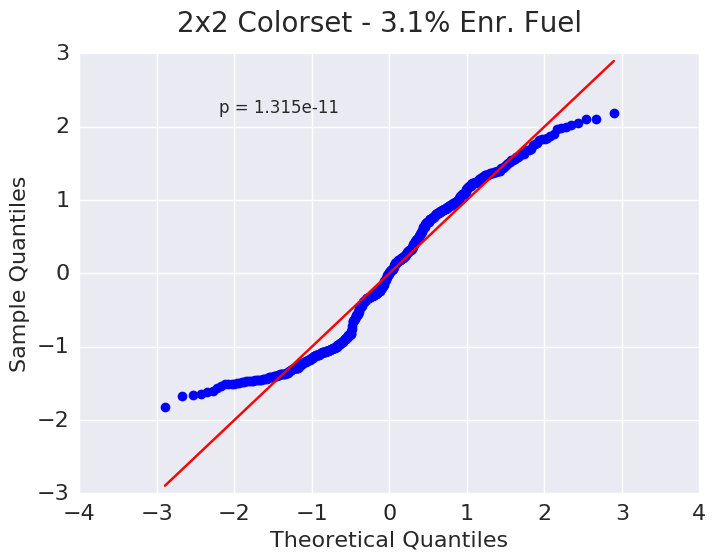
\includegraphics[width=\linewidth]{figures/patterns/2x2/quantile/31-enr-capt-1}
  \caption{}
  \label{fig:chap9-qq-2x2-3.1-capt}
\end{subfigure}
\begin{subfigure}{0.5\textwidth}
  \centering
  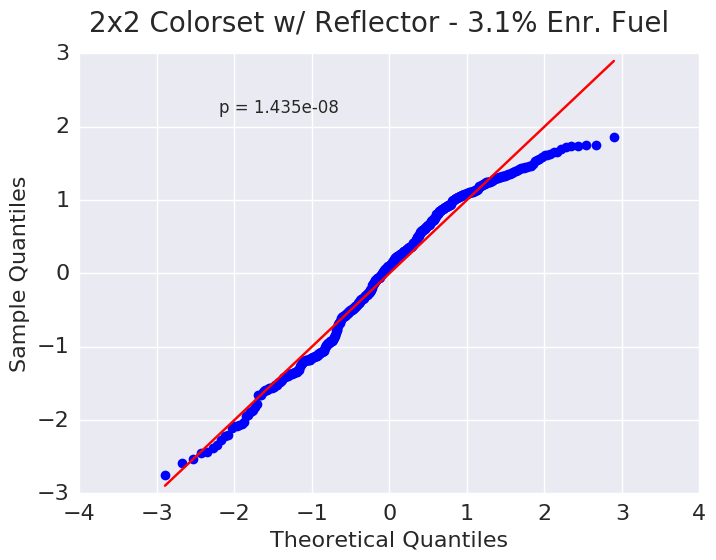
\includegraphics[width=\linewidth]{figures/patterns/reflector/quantile/31-enr-capt-1}  \caption{}
  \label{fig:chap9-qq-reflector-3.1-capt}
\end{subfigure}%
\begin{subfigure}{0.5\textwidth}
  \centering
  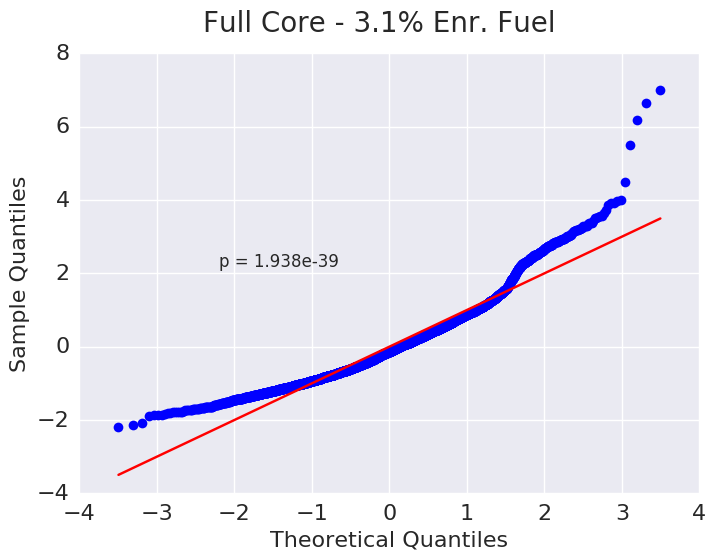
\includegraphics[width=\linewidth]{figures/patterns/full-core/quantile/31-enr-capt-1} \caption{}
  \label{fig:chap9-qq-full-core-3.1-capt}
\end{subfigure}
\caption[Q-Q plots of U-238 capture MGXS for 3.1\% enriched fuel]{\ac{Q-Q} plots of U-238 capture \ac{MGXS} (group 1 of 2) for 3.1\% enriched fuel.}
\label{fig:chap9-qq-3.1-capt}
\end{figure}

At first glance, the larger number of data points (\textit{e.g.}, fuel pin instances) in the \ac{Q-Q} plots for the larger colorset and quarter core benchmarks appear to hide any underlying structure. Although the data points may appear to lie closer to the $y = x$ line for the larger benchmarks, this does not necessarily indicate that the data is more likely to have been drawn from a normal distribution. Indeed, smoothly varying deviations from $y = x$ exhibited in the larger datasets results in smaller $p$-values for the colorset and quarter core models. Of particular note, $p$-values on the order of 10$^{-18}$ and 10$^{-39}$ arise from the data for the 1.6\% and 3.1\% enriched fuel pins, respectively, for the \ac{BEAVRS} quarter core model. These results suggest that it is highly unlikely that the data arose from a normally distributed stochastic process.

%-mention that tails above and below on lower/upper range indicate that tails of distribution are not as wide as would be expected for normal samples -- e.g., a ``tighter'' or ``narrower'' distribution
%-3.1\% enr pins in full core are tighter on bottom edge, but wider on upper edge
%  -indicative of those few ``outlier'' pins with \ac{MGXS} near 0.9 barns in Fig.~\ref{fig:chap9-hist-3.1-capt}

\begin{emphbox}
\textbf{The clustering of U-238 capture \ac{MGXS} manifests itself as ``shoulders'' in \ac{Q-Q} plots. The Shapiro-Wilks test rejects the null hypothesis that the \ac{MGXS} data is drawn from a normal distribution for all six heterogeneous benchmarks.}
\end{emphbox}

%%%%%%%%%%%%%%%%%%%%%%%%%%%%%%%%%%
\subsubsection{U-235 Fission MGXS}
\label{subsubsec:chap9-qq-plots-fiss}

The pin-wise microscopic U-235 fission \ac{MGXS} for 1.6\% and 3.1\% enriched fuel pins are illustrated with histograms and rug plots in Fig.~\ref{fig:chap9-qq-1.6-fiss} and~\ref{fig:chap9-qq-3.1-fiss}, respectively. As was observed in the preceding section for U-238 capture, the datasets for the infinite lattices in Figs.~\ref{fig:chap9-qq-assm-1.6-inf-fiss} and~\ref{fig:chap9-qq-assm-3.1-inf-fiss} appear to be from a normal distribution since they lie very close to the $y = x$ reference line. In addition, the $p$-values are greater than 0.3, well above commonly used significance levels; thus one would not reject the null hypothesis that the data is from a normal distribution.

\begin{figure}[h!]
\centering
\begin{subfigure}{0.5\textwidth}
  \centering
  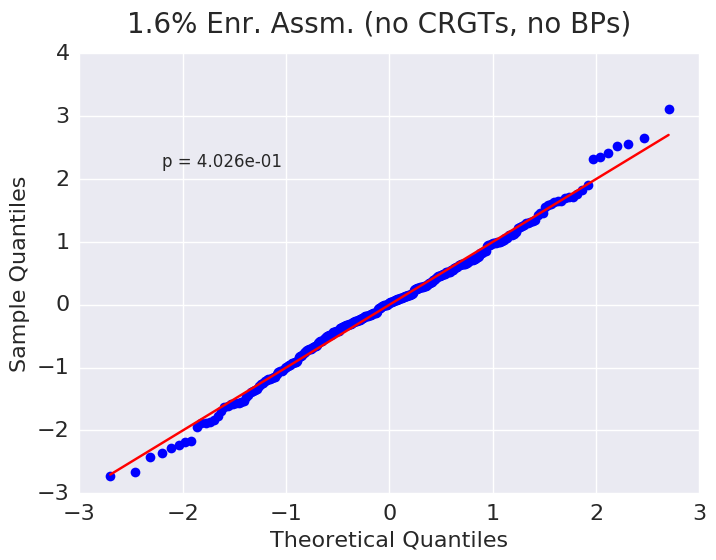
\includegraphics[width=\linewidth]{figures/patterns/assm-1.6-inf/quantile/assm-16-inf-fiss-2}
  \caption{}
  \label{fig:chap9-qq-assm-1.6-inf-fiss}
\end{subfigure}%
\begin{subfigure}{0.5\textwidth}
  \centering
  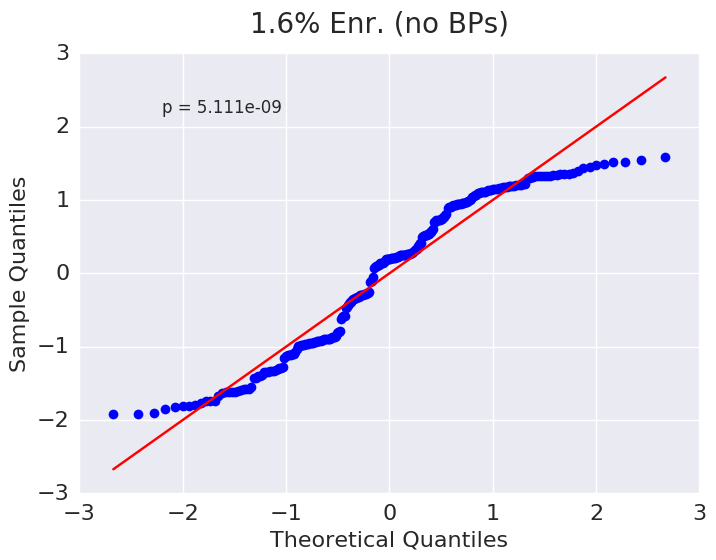
\includegraphics[width=\linewidth]{figures/patterns/assm-1.6/quantile/assm-16-fiss-2}
  \caption{}
  \label{fig:chap9-qq-assm-1.6-fiss}
\end{subfigure}
\begin{subfigure}{0.5\textwidth}
  \centering
  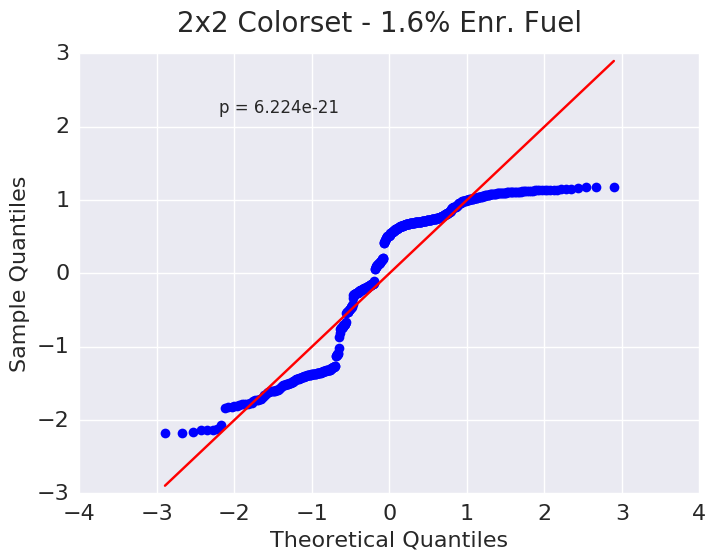
\includegraphics[width=\linewidth]{figures/patterns/2x2/quantile/16-enr-fiss-2}
  \caption{}
  \label{fig:chap9-qq-2x2-1.6-fiss}
\end{subfigure}%
\begin{subfigure}{0.5\textwidth}
  \centering
  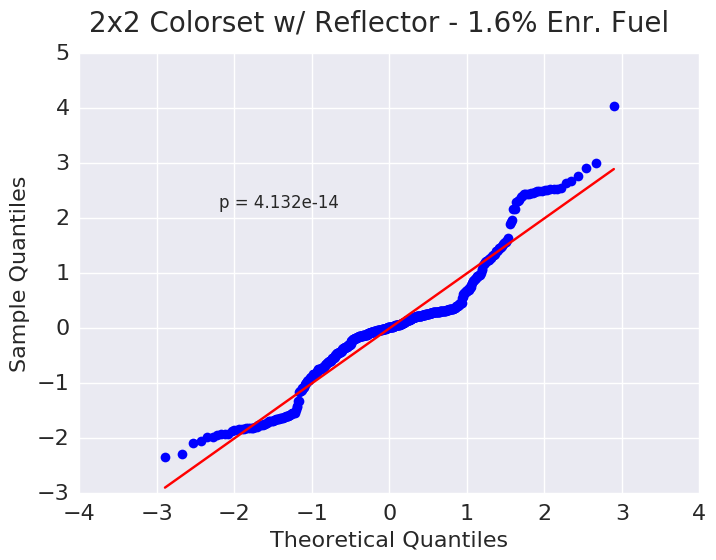
\includegraphics[width=\linewidth]{figures/patterns/reflector/quantile/16-enr-fiss-2}  \caption{}
  \label{fig:chap9-qq-reflector-1.6-fiss}
\end{subfigure}
\begin{subfigure}{0.5\textwidth}
  \centering
  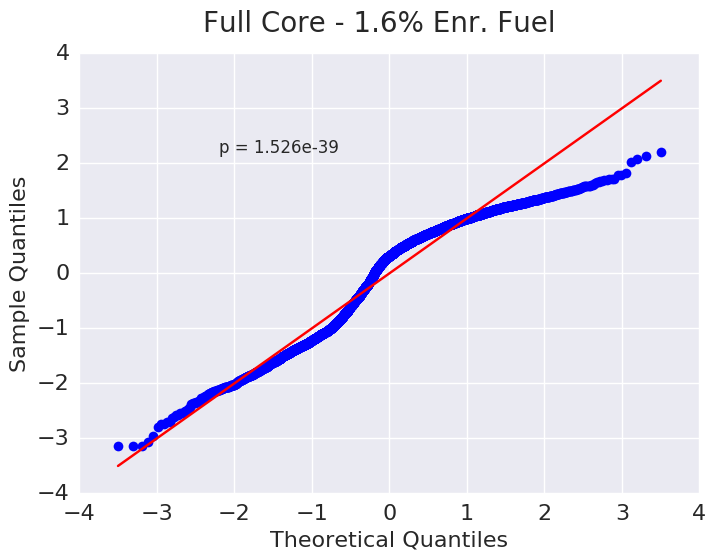
\includegraphics[width=\linewidth]{figures/patterns/full-core/quantile/16-enr-fiss-2} \caption{}
  \label{fig:chap9-qq-full-core-1.6-fiss}
\end{subfigure}
\caption[Q-Q plots of U-235 fission MGXS for 1.6\% enriched fuel]{\ac{Q-Q} plots of U-235 fission \ac{MGXS} (group 2 of 2) for 1.6\% enriched fuel.}
\label{fig:chap9-qq-1.6-fiss}
\end{figure}

\begin{figure}[h!]
\centering
\begin{subfigure}{0.5\textwidth}
  \centering
  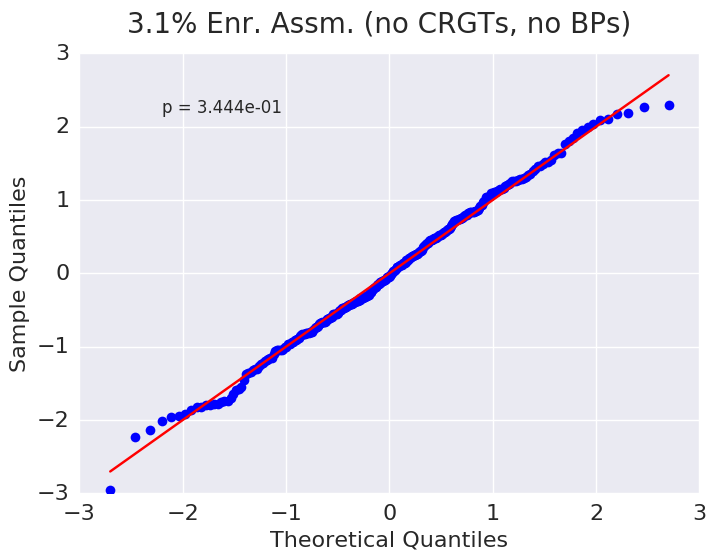
\includegraphics[width=\linewidth]{figures/patterns/assm-3.1-inf/quantile/assm-31-inf-fiss-2}
  \caption{}
  \label{fig:chap9-qq-assm-3.1-inf-fiss}
\end{subfigure}%
\begin{subfigure}{0.5\textwidth}
  \centering
  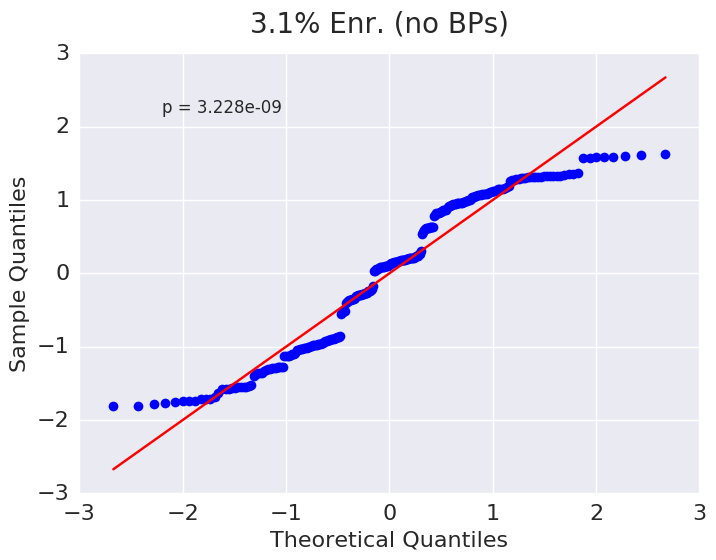
\includegraphics[width=\linewidth]{figures/patterns/assm-3.1/quantile/assm-31-fiss-2}
  \caption{}
  \label{fig:chap9-qq-assm-3.1-fiss}
\end{subfigure}
\begin{subfigure}{0.5\textwidth}
  \centering
  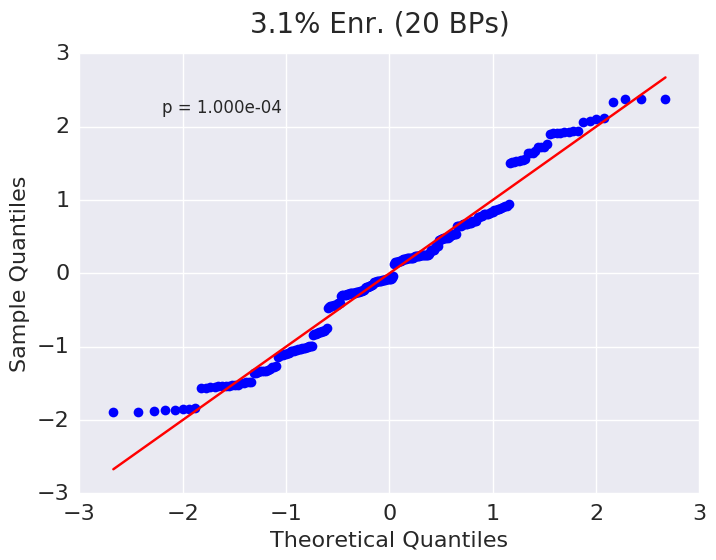
\includegraphics[width=\linewidth]{figures/patterns/assm-3.1-20BPs/quantile/assm-31-20BPs-fiss-2}
  \caption{}
  \label{fig:chap9-qq-assm-3.1-20BPs-fiss}
\end{subfigure}%
\begin{subfigure}{0.5\textwidth}
  \centering
  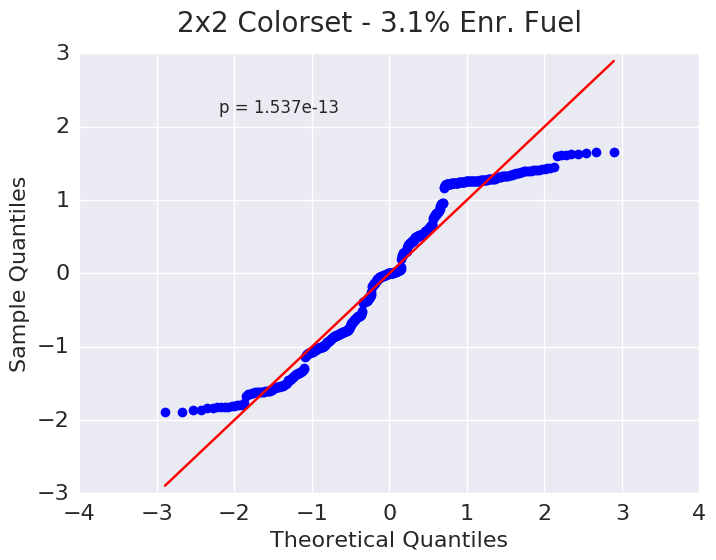
\includegraphics[width=\linewidth]{figures/patterns/2x2/quantile/31-enr-fiss-2}
  \caption{}
  \label{fig:chap9-qq-2x2-3.1-fiss}
\end{subfigure}
\begin{subfigure}{0.5\textwidth}
  \centering
  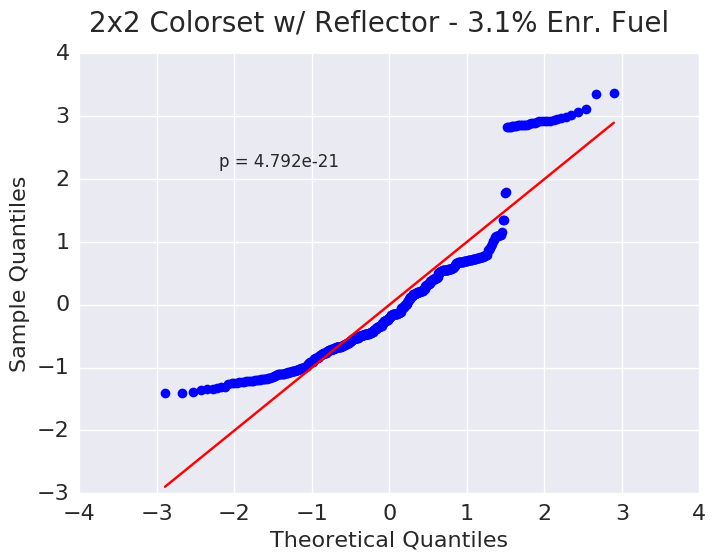
\includegraphics[width=\linewidth]{figures/patterns/reflector/quantile/31-enr-fiss-2}  \caption{}
  \label{fig:chap9-qq-reflector-3.1-fiss}
\end{subfigure}%
\begin{subfigure}{0.5\textwidth}
  \centering
  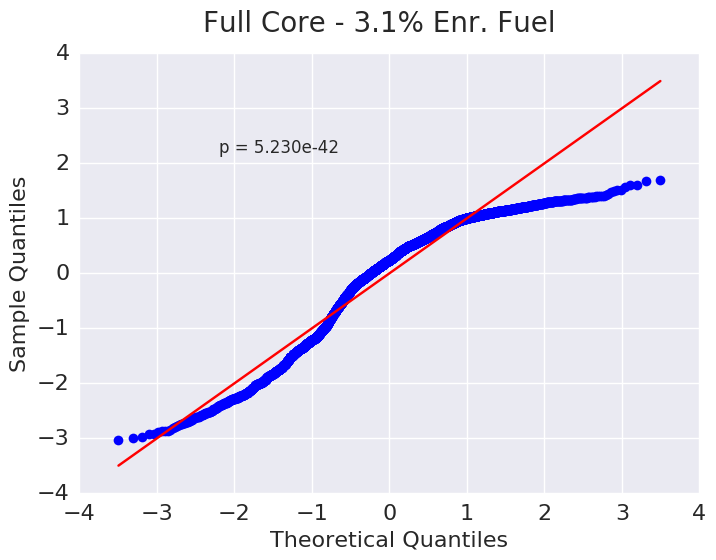
\includegraphics[width=\linewidth]{figures/patterns/full-core/quantile/31-enr-fiss-2} \caption{}
  \label{fig:chap9-qq-full-core-3.1-fiss}
\end{subfigure}
\caption[Q-Q plots of U-235 fission MGXS 3.1\% enriched fuel]{\ac{Q-Q} plots of U-235 fission \ac{MGXS} (group 2 of 2) for 3.1\% enriched fuel.}
\label{fig:chap9-qq-3.1-fiss}
\end{figure}

The addition of \acp{CRGT} leads to a clear deviation from normality in Figs.~\ref{fig:chap9-qq-assm-1.6-fiss} and~\ref{fig:chap9-qq-assm-3.1-fiss}. However, the structure is substantially more complex than the four shoulders exhibited in the U-238 capture \ac{MGXS} data. As was noted in Sec.~\ref{subsubsec:chap9-histograms-fiss}, the presence of \acp{BP} results in many distinct clusters which appear as a highly fragmented, step-like profile in the \ac{Q-Q} plot in Fig.~\ref{fig:chap9-qq-assm-3.1-20BPs-capt}. The high degree of clustering exhibited in the histograms and rug plots for the larger colorset and quarter core benchmarks similarly appears in the corresponding \ac{Q-Q} plots.

As noted for the U-238 capture \ac{MGXS}, the $p$-values for the Shapiro-Wilks tests of the pin-wise U-235 fission \ac{MGXS} data affirm the deviation from normality seen in the \ac{Q-Q} plots. Of particular note, $p$-values on the order of 10$^{-38}$ and 10$^{-43}$ arise from the data for the 1.6\% and 3.1\% enriched fuel pins, respectively, for the \ac{BEAVRS} quarter core model. These results suggest that it is highly unlikely that the data arose from a normally distributed stochastic process.

%-mention that tails above and below on lower/upper range indicate that tails of distribution are not as wide as would be expected for normal samples -- e.g., a ``tighter'' or ``narrower'' distribution
%-3.1\% enr pins in full core are tighter on bottom edge, but wider on upper edge
%  -indicative of those few ``outlier'' pins with \ac{MGXS} near 0.9 barns in Fig.~\ref{fig:chap9-hist-3.1-capt}

\begin{emphbox}
\textbf{The higher degree of clustering of pin-wise U-235 fission \ac{MGXS} than U-238 capture \ac{MGXS} results in highly fragmented step-like \ac{Q-Q} plots. The Shapiro-Wilks test once again rejects the null hypothesis that the \ac{MGXS} data is drawn from a normal distribution for all six heterogeneous benchmarks.}
\end{emphbox}


%%%%%%%%%%%%%%%%%%%%%%%%%%%%%%%%%%%%%%%%%%%%%%%%%%%%%%%%%%%%%%%%%%%%%%%%%%%%%%%
\section{LNS Spatial Homogenization}
\label{sec:chap9-lns-homogenize}

The preceding sections quantified and visualized the dispersion and structural clustering of pin-wise \ac{MGXS} due to spatial self-shielding effects. The degenerate spatial homogenization scheme evaluated in Chap.~\ref{chap:quantify} is able to model the clustering of \ac{MGXS} by assigning a unique set of \ac{MGXS} to each fuel pin instance in a core geometry. However, the infinite and null schemes fail to account for \ac{MGXS} clustering since they each assign a single \ac{MGXS} to all instances of the same fuel pin type. As evidenced by the results in Chap.~\ref{chap:quantify}, it is important to adequately model clusters of pin-wise \ac{MGXS} in order to accurately predict U-238 capture rate spatial distributions. 

This section introduces a new spatial homogenization scheme which uses a deterministic approach to cluster pin-wise \ac{MGXS} based on an analysis of the core geometry. The approach developed here is akin to geometric templates employed by some commonly used lattice physics codes, such as CASMO~\cite{rhodes2006casmo}, to predict which groupings of pins are likely to experience similar spatial self-shielding effects and hence have similar microscopic \ac{MGXS}. The new scheme is termed \textit{\ac{LNS} homogenization} since it is predicated upon OpenCG's Local Neighbor Symmetry (LNS) algorithm (see Sec.~\ref{sec:chap4-lns}). The \ac{LNS} algorithm analyzes the combinatorial geometry (CG) used to represent each benchmark model and groups pins together based on their neighboring spatial zones. The goal of \ac{LNS} homogenization is to achieve degenerate homogenization's predictive accuracy by representing \ac{MGXS} clustering, and approach null homogenization's tally convergence by homogenizing \ac{MGXS} across many pin instances.

%%%%%%%%%%%%%%%%%%%%%
\subsection{Overview}
\label{subsec:chap9-lns-overview}

Like the degenerate spatial homogenization scheme (Sec.~\ref{subsec:chap8-degenerate}), a single \ac{MC} calculation of the complete heterogeneous geometry is used to generate \ac{MGXS} for all materials. The \ac{MGXS} are tallied separately for each instance of fissile material zones using OpenMC's distributed cell tallies (see Sec.~\ref{subsec:chap4-distribcells}). The OpenCG \ac{LNS} algorithm assigns an integral \ac{LNS} identifier to each unique pin instance in the \ac{CG} based on an analysis of each pin's neighbors at each level of the \ac{CG} hierarchy. Pins with like neighboring pins, within assemblies with like neighboring assemblies, will receive the same \ac{LNS} identifier\footnote{\ac{LNS} hashes a data structure representing a rotationally invariant form of each pin's neighbors.}. The \ac{MGXS} are averaged across all pin instances with the same unique \ac{LNS} identifier. For example, all pins adjacent to a single \ac{CRGT} on one face and fuel pins on all other faces are assigned the same \ac{MGXS} averaged across the OpenMC distributed cell tallies for all of those pin instances. The OpenCG region differentiation algorithm (see Sec.~\ref{sec:chap4-region-diff}) is used to build an OpenMOC geometry with unique cells and materials for each fuel pin which mirrors the \ac{LNS} representation of the \ac{CG} model. Like the infinite, null and degenerate schemes, spatial self-shielding effects experienced by different non-fissile spatial zones are averaged across the entire geometry for each non-fissile material.

The total number of materials (\textit{i.e.}, \ac{MGXS}) used to model each benchmark with the \ac{LNS} homogenization scheme is given in Tab.~\ref{fig:chap9-lns-materials}. The fuel assemblies with \acp{CRGT} and \acp{BP} and 2$\times$2 colorset benchmark models are color-coded by material and illustrated in Fig.~\ref{fig:chap9-lns-materials} for the \ac{LNS} homogenization scheme. Likewise, the materials for the quarter core \ac{BEAVRS} model with \ac{LNS} homogenization is highlighted in Fig.~\ref{fig:chap9-lns-materials-beavrs}. 

\begin{table}[h!]
  \centering
  \caption[Number of materials for LNS spatial homogenization]{Number of materials modeled with unique \ac{MGXS} in each heterogeneous benchmark for \ac{LNS} spatial homogenization.}
  \small
  \label{table:chap9-num-materials-lns}
  \vspace{6pt}
  \begin{tabular}{l r r r}
  \toprule
  \rowcolor{lightgray}
  & \multicolumn{3}{c}{\cellcolor{lightgray} \bf \# Fuel Materials} \\
  \multirow{-2}{*}{\cellcolor{lightgray} \bf Benchmark} &
  \multicolumn{1}{c}{\cellcolor{lightgray} \bf Null/Infinite} &
  \multicolumn{1}{c}{\cellcolor{lightgray} \bf \ac{LNS}} &
  \multicolumn{1}{c}{\cellcolor{lightgray} \bf Degenerate} \\
  \midrule
1.6\% Assm & 1 & 9 & 264 \\
%1.6\% Assm & 5 & 13 & 268 \\
3.1\% Assm & 1 & 9 & 264 \\
%3.1\% Assm & 5 & 13 & 268 \\
3.1\% Assm w/ 20 BPs & 1 & 10 & 264  \\
%3.1\% Assm w/ 20 BPs & 7 & 17 & 270  \\
2$\times$2 Colorset & 2 & 19 & 1,056 \\
%2$\times$2 Colorset & 8 & 25 & 1,062 \\
2$\times$2 Colorset w/ Reflector & 2 & 29 & 1,056 \\
%2$\times$2 Colorset w/ Reflector & 8 & 35 & 1,062 \\
\ac{BEAVRS} Quarter Core & 3 & 495 & 12,993 \\ % LNS = ceil(193 / 4) * 10 + 7 - actually just counted them %\ac{BEAVRS} Quarter Core & 10 & 502 & 13,000 \\ % LNS = ceil(193 / 4) * 10 + 7 - actually just counted them up as 10 for assms with BPs and 8 otherwise
  \bottomrule
\end{tabular}
\end{table}

\begin{figure}[h!]
\centering
\begin{subfigure}{.45\textwidth}
  \centering
  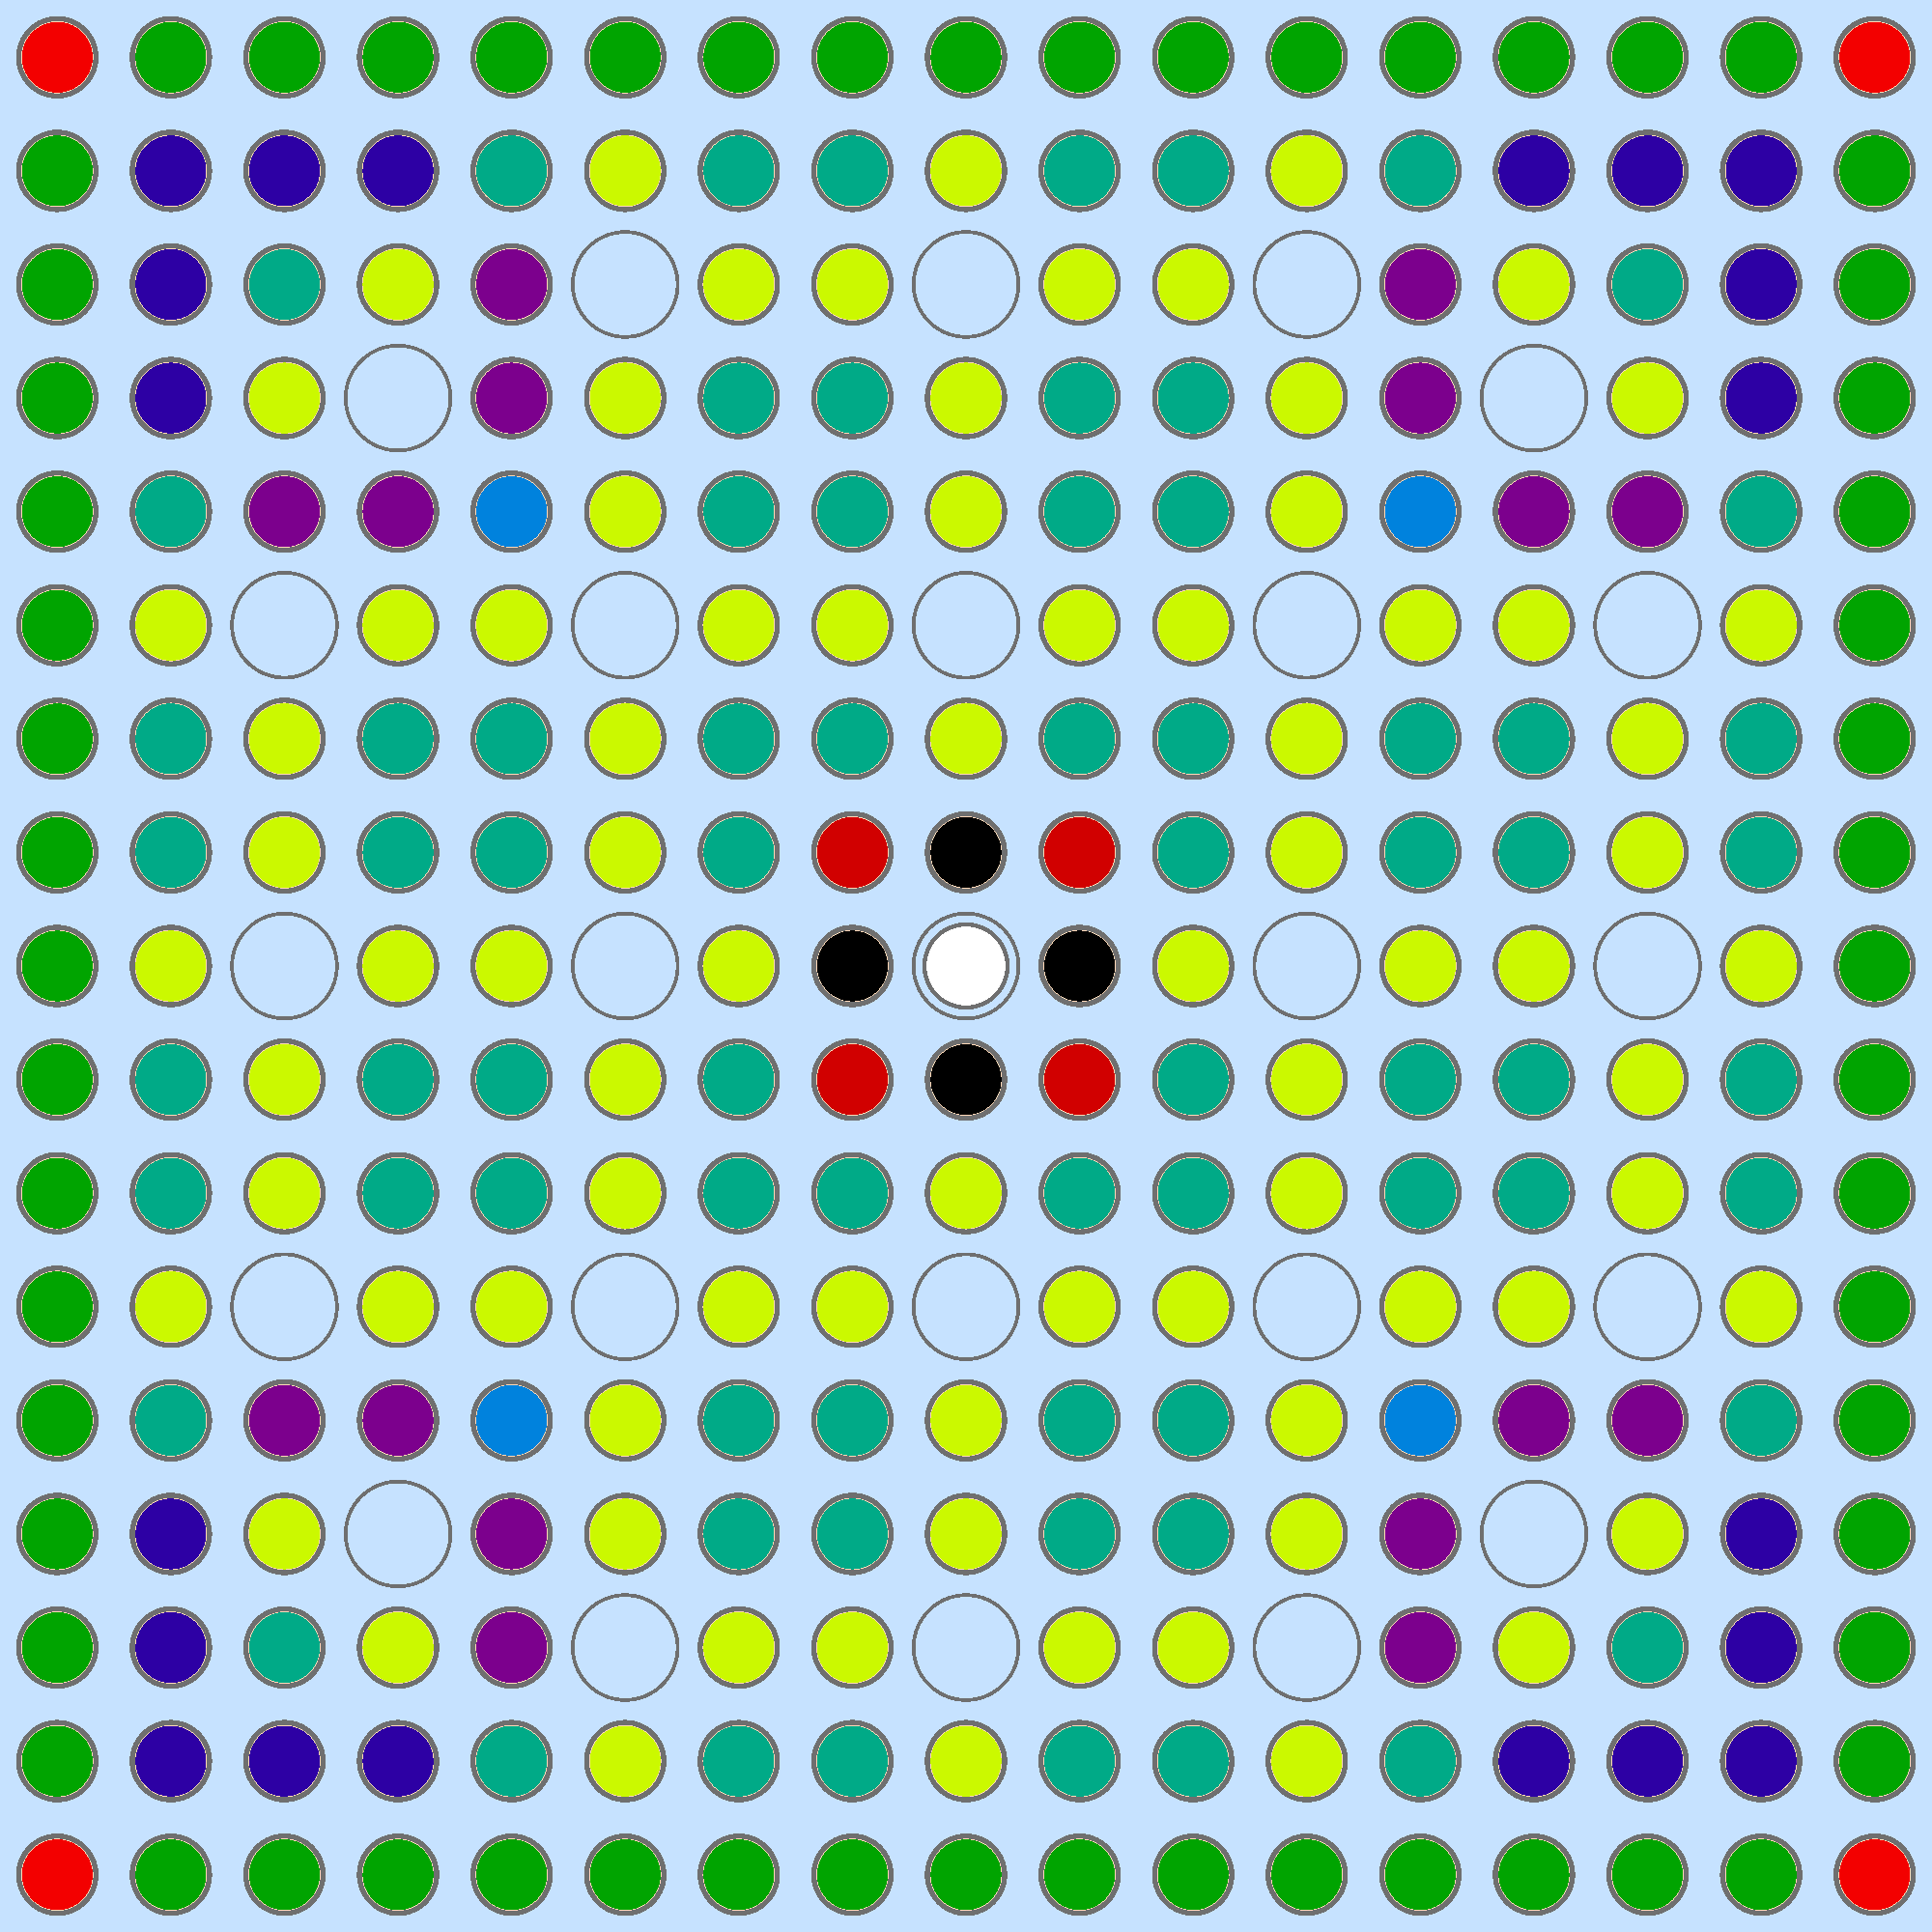
\includegraphics[width=0.9\linewidth]{figures/patterns/lns/assm-31/materials}
  \caption{}
  \label{fig:chap9-assm-31-lns-materials}
\end{subfigure}%
\begin{subfigure}{.45\textwidth}
  \centering
  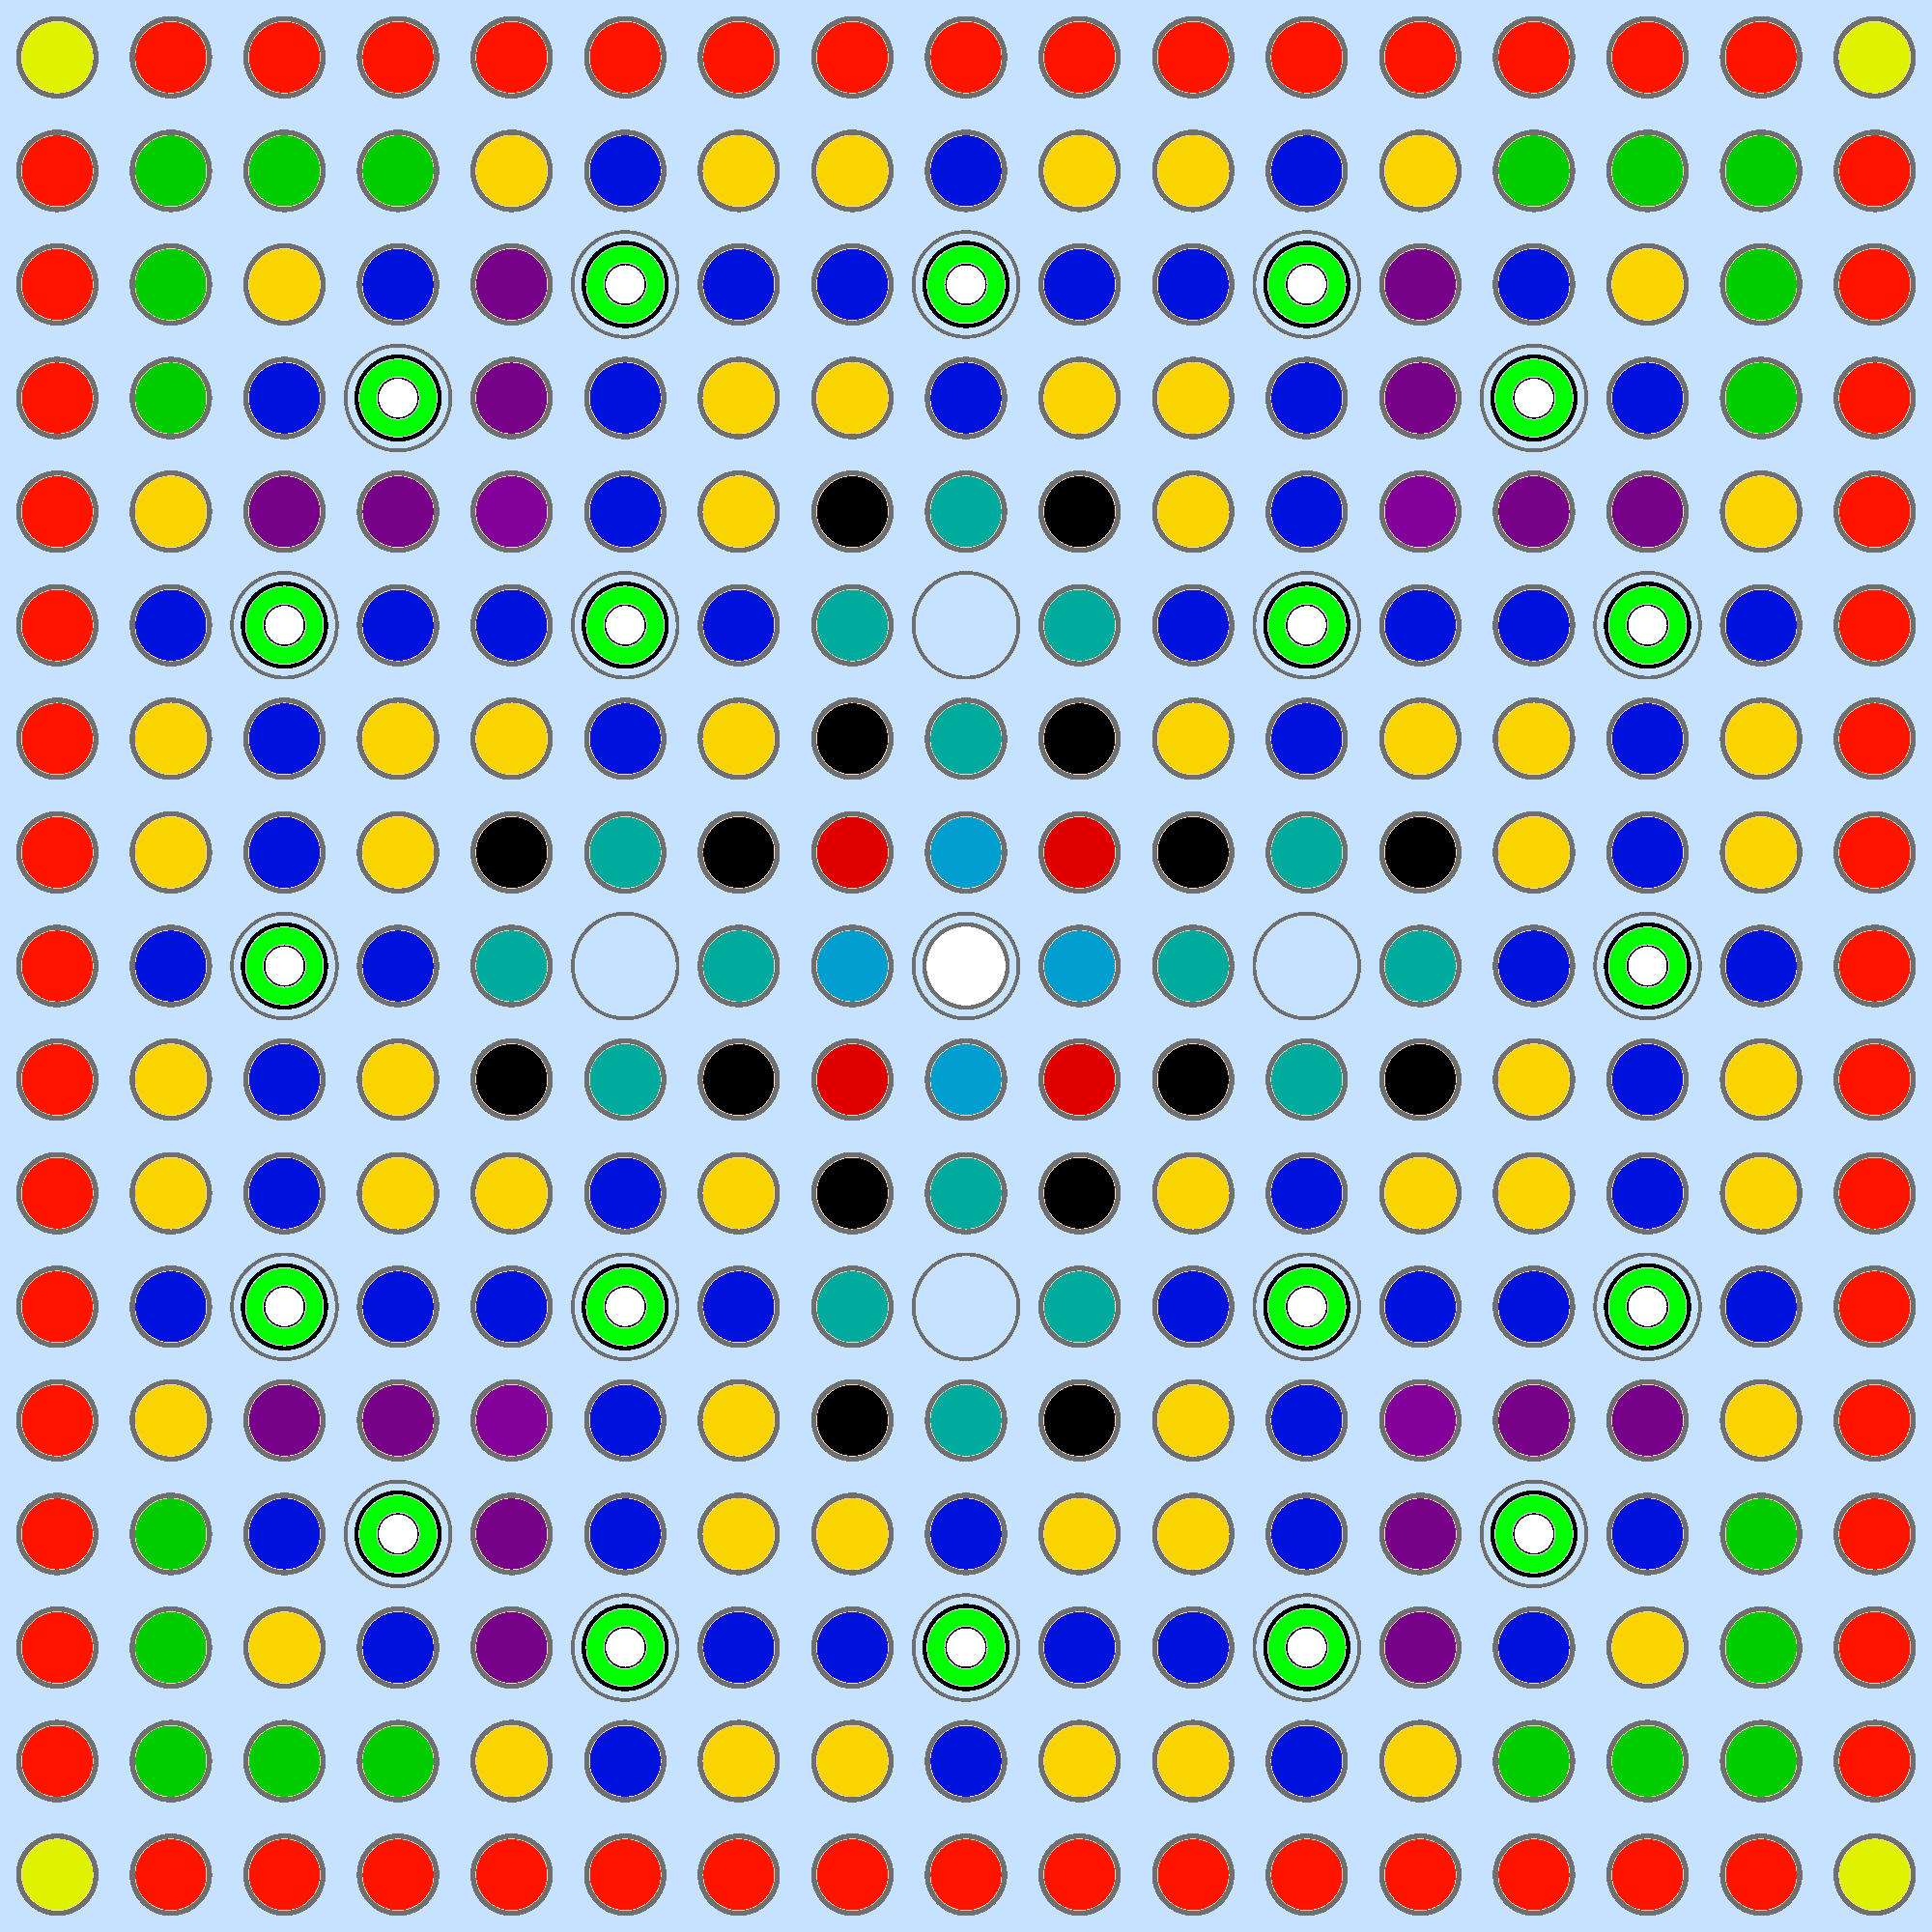
\includegraphics[width=0.9\linewidth]{figures/patterns/lns/assm-31-20BPs/materials}
  \caption{}
  \label{fig:chap9-31-20BPs-lns-materials}
\end{subfigure}
\begin{subfigure}{.45\textwidth}
  \centering
  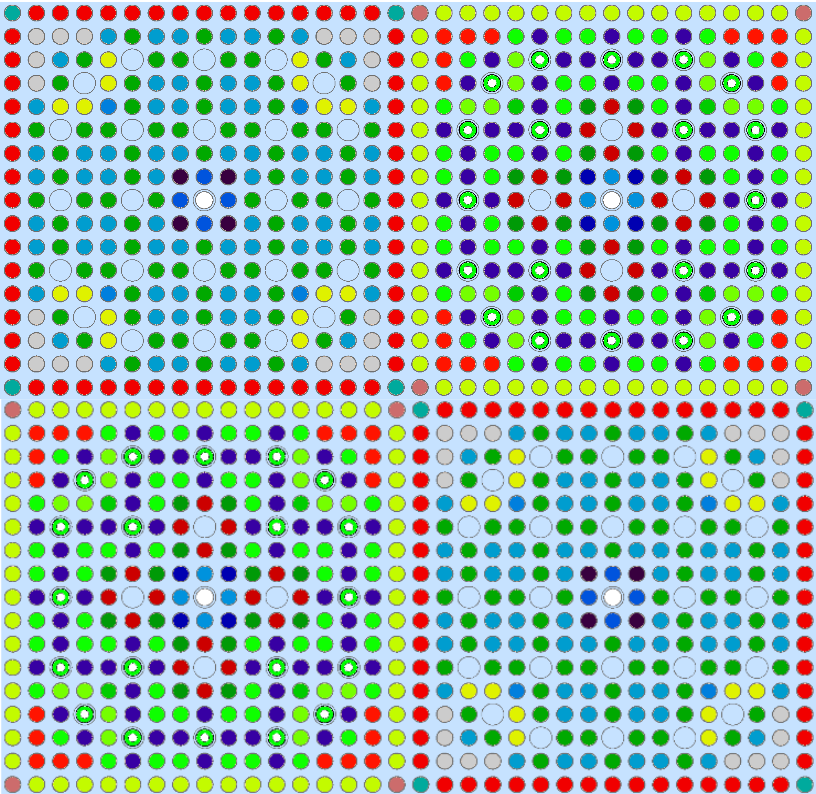
\includegraphics[width=0.9\linewidth]{figures/patterns/lns/2x2/materials}
  \caption{}
  \label{fig:chap9-2x2-lns-materials}
\end{subfigure}%
\begin{subfigure}{.45\textwidth}
  \centering
  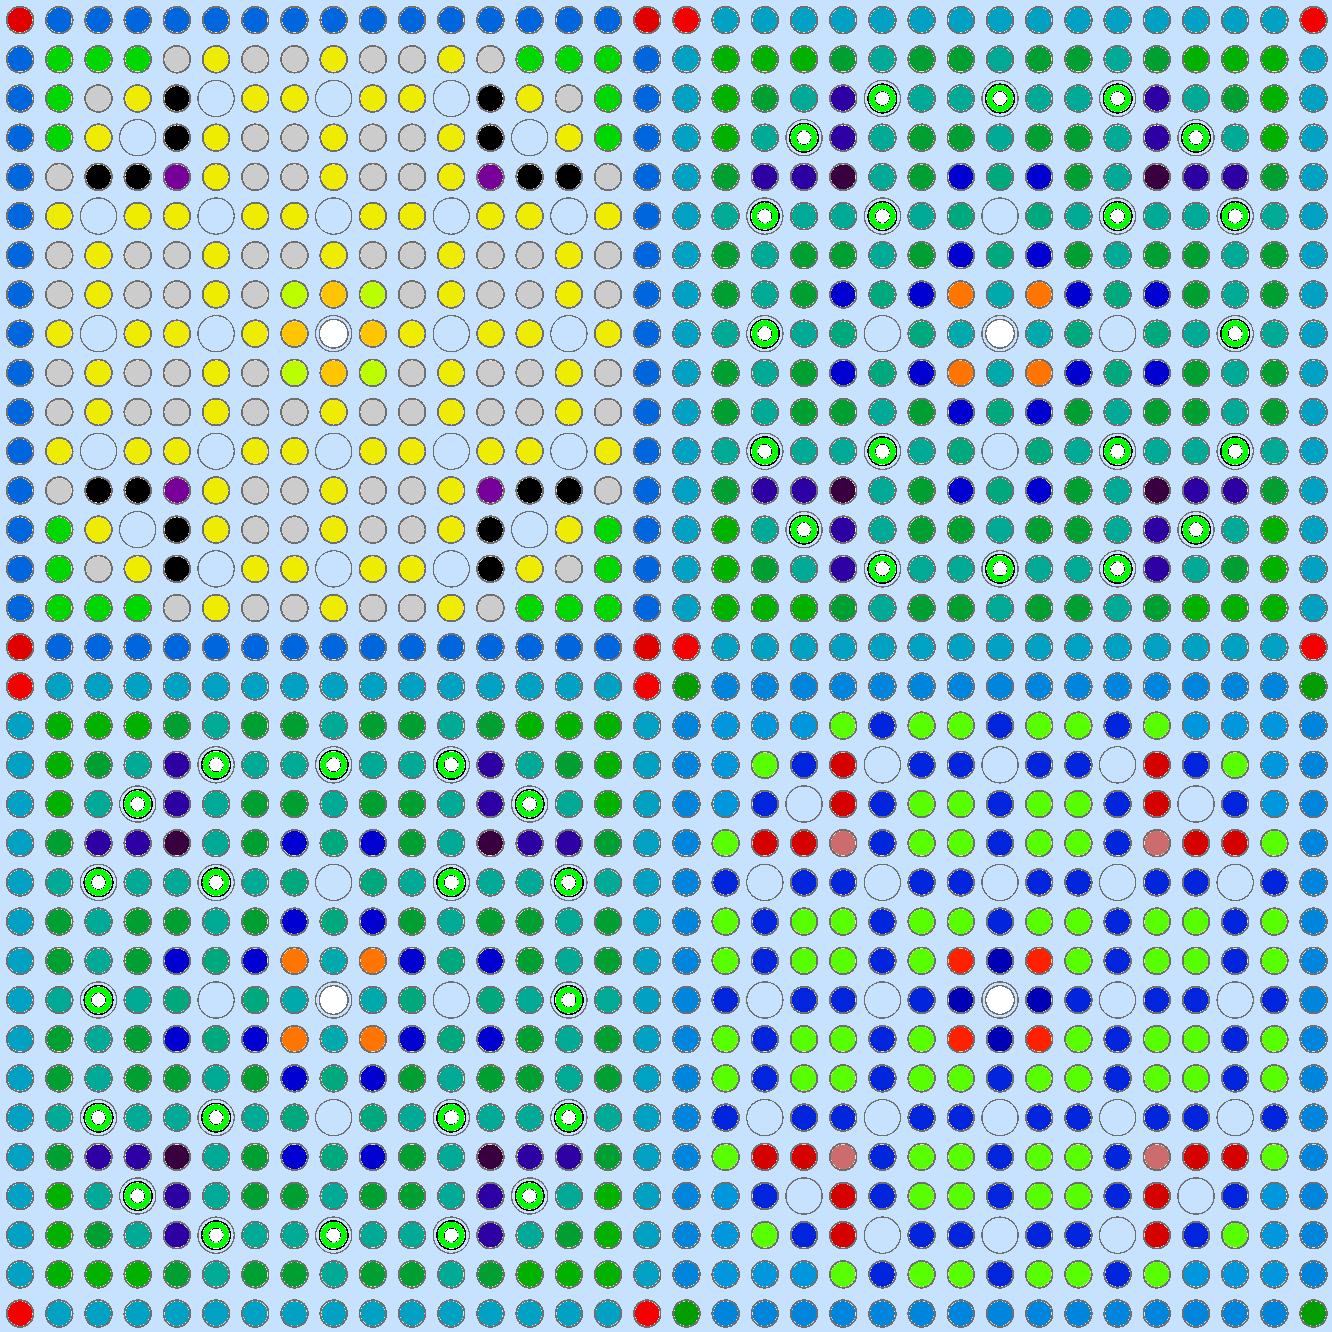
\includegraphics[width=0.9\linewidth]{figures/patterns/lns/reflector/materials}
  \caption{}
  \label{fig:chap9-reflector-lns-materials}
\end{subfigure}
\caption[Depiction of LNS spatially homogenized materials]{OpenMOC materials with \ac{LNS} spatial homogenization for an assembly with \acp{CRGT} (a), an assembly with 20 \acp{BP} (b), a 2$\times$2 colorset without (c) and with (d) a reflector. Each uniquely colored material represents a unique set of \ac{MGXS}.}
\label{fig:chap9-lns-materials}
\end{figure}

\begin{figure}[h!]
\centering
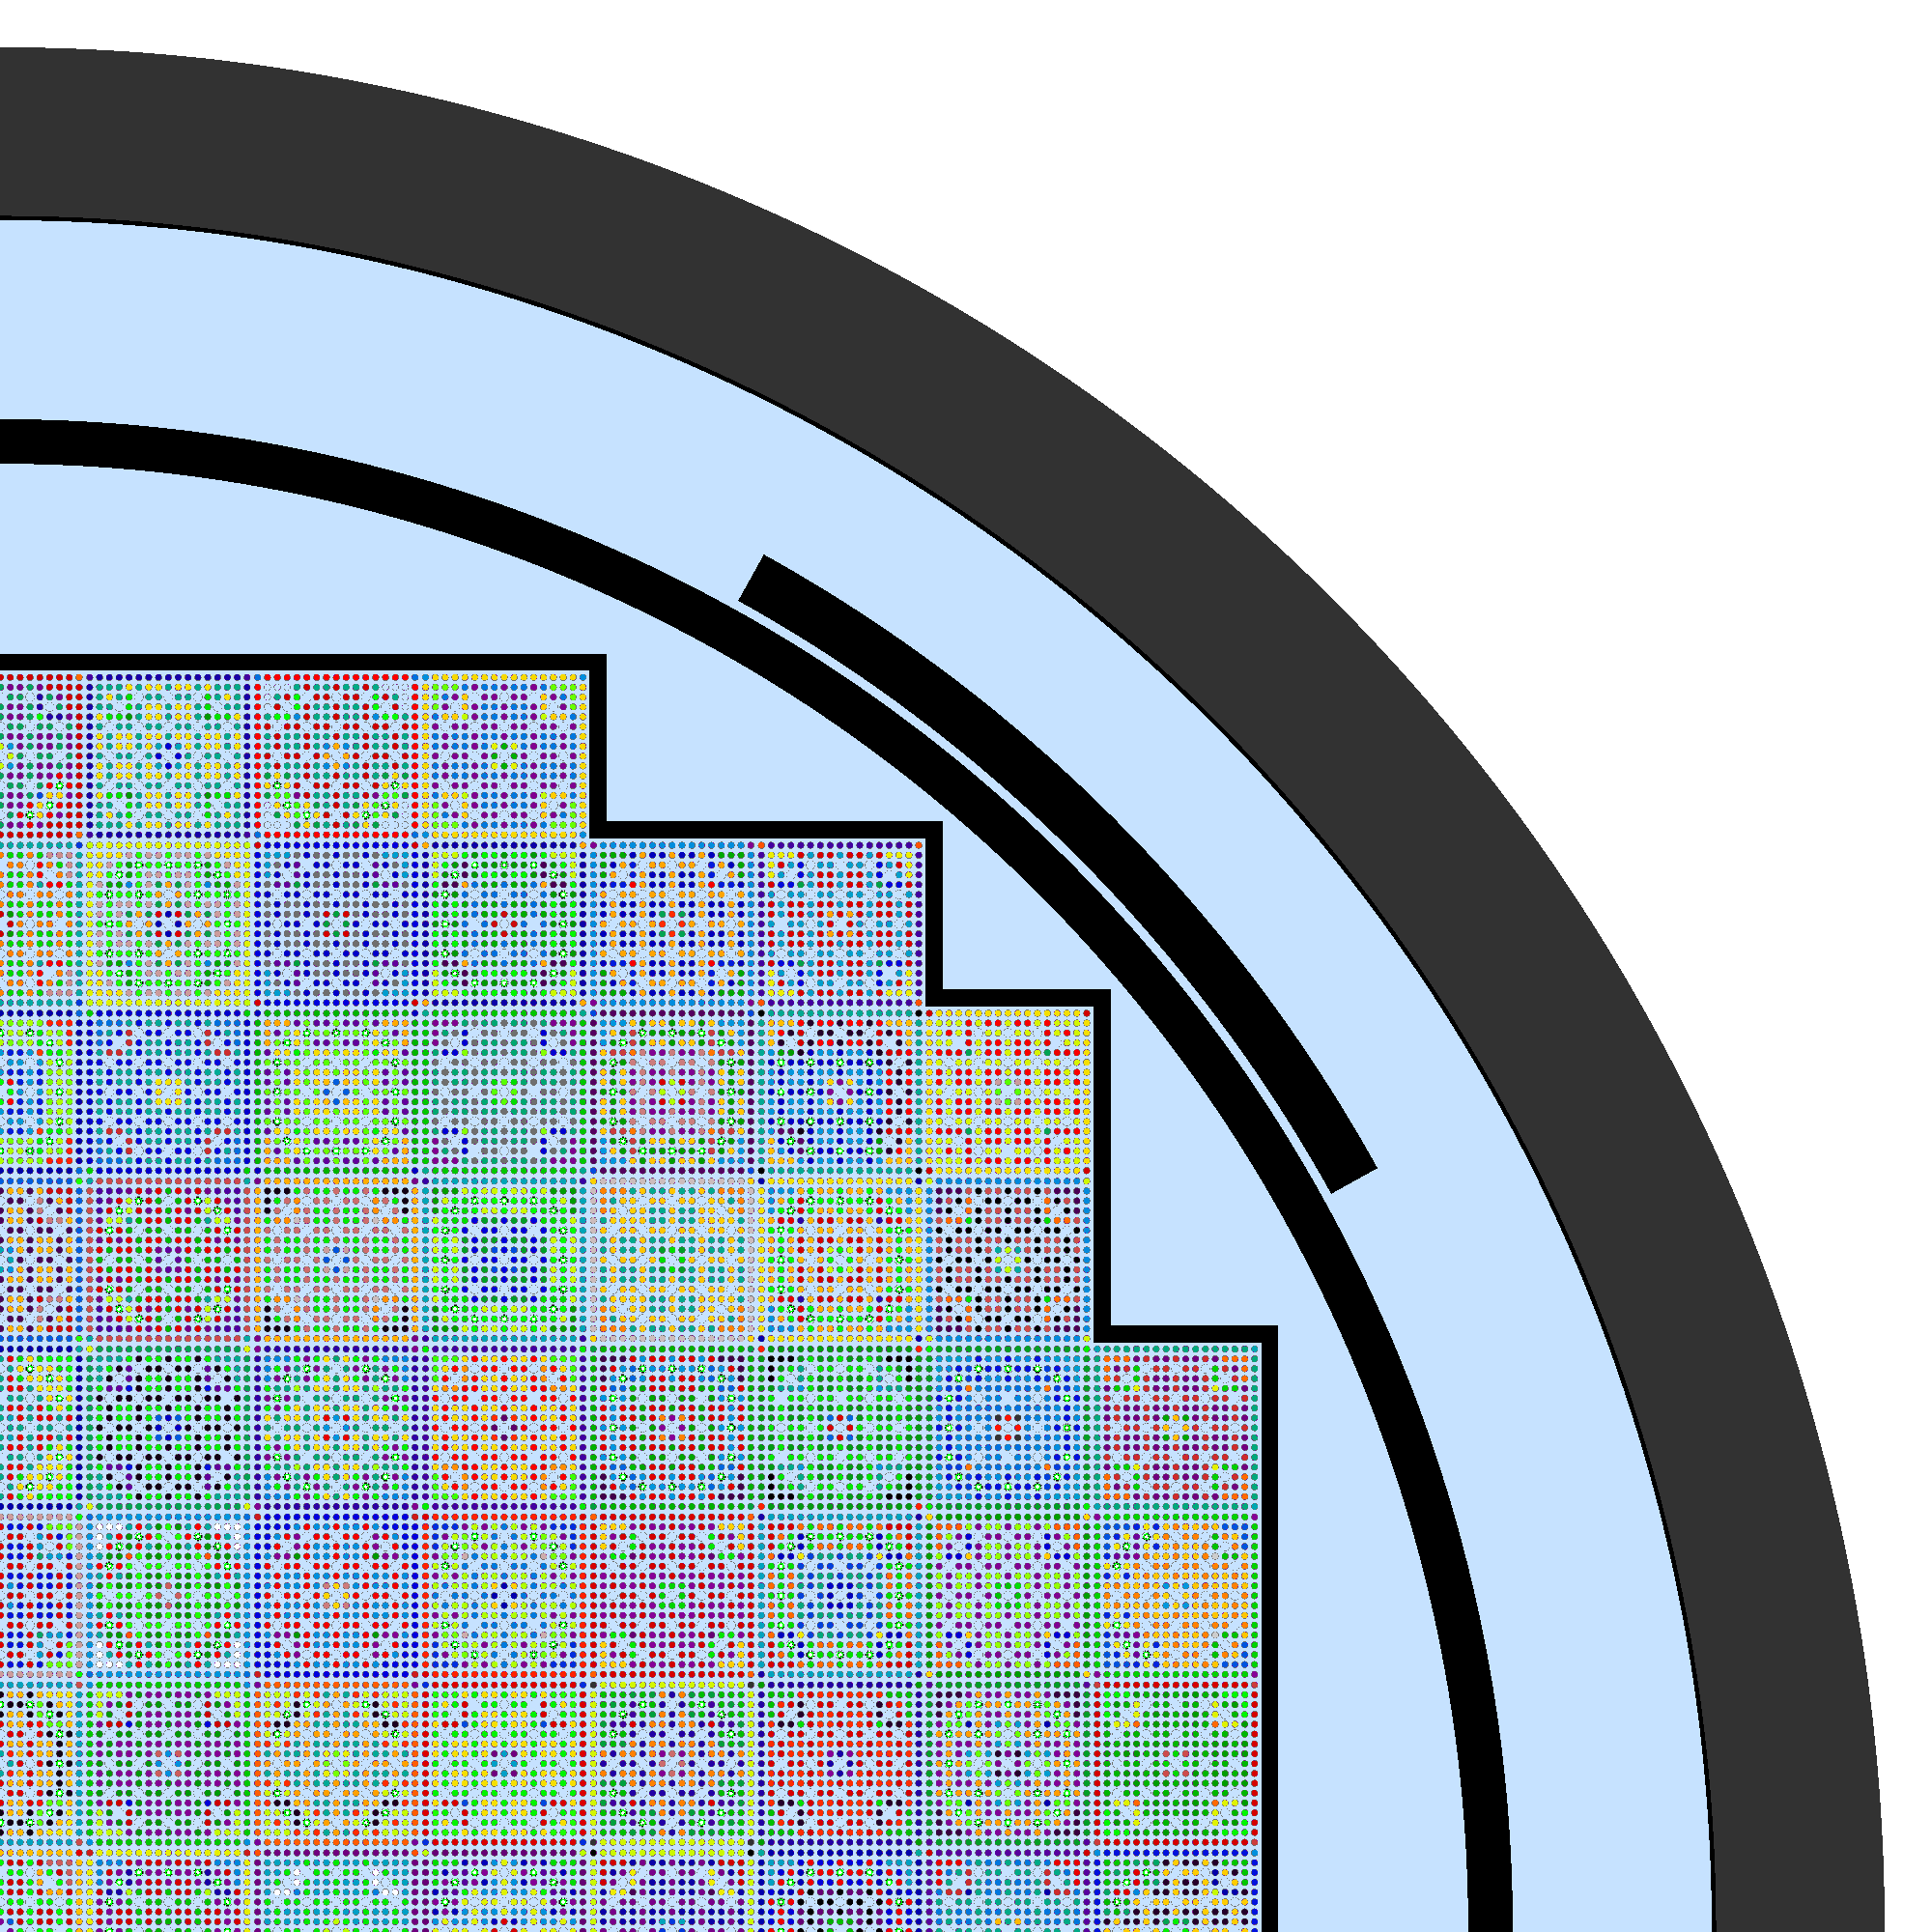
\includegraphics[width=\linewidth]{figures/patterns/lns/full-core/materials}
\vspace{2mm}
\caption[Depiction of LNS spatially homogenized materials for BEAVRS]{OpenMOC materials with \ac{LNS} spatial homogenization for the 2D quarter core \ac{BEAVRS} model. Each uniquely colored material represents a unique set of \ac{MGXS}.}
\label{fig:chap9-lns-materials-beavrs}
\end{figure}

As quantified in the Tab.~\ref{table:chap9-num-materials-lns}, 9 -- 10 unique fissile materials are used for each fuel assembly with \ac{LNS}, far fewer than the 264 in degenerate homogenization. Consequently, the \ac{MC} tallies for \ac{LNS} homogenization will converge more quickly than those for degenerate homogenization. In addition, as indicated by the figures, fuel pin types with neighboring heterogeneities are assigned unique \ac{MGXS} which generally reflects the clustering of \ac{MGXS} due to spatial self-shielding effects. As a result, \ac{LNS} homogenization would be expected to enable more accurate predictions of reaction rate distributions than is possible with the null scheme. 

%%%%%%%%%%%%%%%%%%%%%%%%%%%%%%%%%%%%%%%%
\subsection{Track Density-Weighted MGXS}
\label{subsec:chap9-lns-math}

The \ac{LNS} spatially-homogenized \ac{MGXS} for each group of pin instances are not simply computed as the geometric average of the \ac{MGXS} in each pin instance. Instead, the total reaction rates and fluxes in each pin instance are first summed together and then divided to compute an average \ac{MGXS} which is effectively weighted by the relative particle track density in each fuel pin instance. The track density-weighted average \ac{MGXS} preserve global reaction rates\footnote{A simple geometric average of \ac{MGXS} across fuel pins will not preserve global reaction rates.} and are equivalent to defining specialized OpenMC ``cell'' reaction rate and flux tallies for each group of pin instances with like \ac{LNS} identifiers. In order to formally express the track density weighted-average approach, it is useful to first recall Eqn.~\ref{eqn:chap3-general-micro} for a microscopic \ac{MGXS} estimated from \ac{MC} tallies for reaction $x$, nuclide $i$, spatial zone $k$ and energy group $g$:

\begin{equation}
\label{eqn:chap9-general-micro}
\hat{\sigma}_{x,i,k,g} = \frac{\langle \sigma_{x,i}, \psi \rangle_{k,g}^{t\ell}}{\langle \psi \rangle_{k,g}^{t\ell}}
\end{equation}

\noindent In this context, the index $k$ of $K$ total spatial zones refers to a particular instance of a fuel pin within a core geometry. The \ac{LNS} algorithm represents a function $S(k)$ which assigns an identifier $m$ to each fuel pin instance based on its neighbors (\textit{i.e.}, pin instances with the same neighbors are assigned the same identifier). The set $\mathbb{S}_{m}$ encapsulates all instances $k$  with the same \ac{LNS} identifier:

\begin{equation}
\label{eqn:chap9-lns-set}
\mathbb{S}_{m} = \left\{1 \le k \le K: S(k) = m\right\}
\end{equation}

\ac{LNS} homogenization computes a single set of \ac{MGXS} for the fuel pin instances in each set $k \in \mathbb{S}_{m}$ classified by the \ac{LNS} algorithm. This is equivalent to a specialization of Eqn.~\ref{eqn:chap9-general-micro} with track density-weighted averages of the reaction rates and flux tallies in each pin instance:

\begin{equation}
\label{eqn:chap9-lns-micro}
\hat{\sigma}_{x,i,m,g} = \frac{\displaystyle\sum\limits_{k=1}^{K}\mathbb{1}_{\mathbb{S}_{m}}(k) \langle \sigma_{x,i}, \psi \rangle_{k,g}^{t\ell}}{\displaystyle\sum\limits_{k=1}^{K}\mathbb{1}_{\mathbb{S}_{m}}(k) \langle \psi \rangle_{k,g}^{t\ell}}
\end{equation}

\noindent where the indicator function $\mathbb{1}_{\mathbb{S}_{m}}(k)$ is equal to 1 if $k \in \mathbb{S}_{m}$ and 0 otherwise. The track density-weighted average is similarly applied to the \ac{MC} tallies for each type of \ac{MGXS}, including scattering matrices and the fission spectrum.

%%%%%%%%%%%%%%%%%%%%%%%%%%%%%%%%%%%%%%%%
\subsection{Potential Shortcomings}
\label{subsec:chap9-lns-shortcomings}

Upon further inspection, it is clear from Figs. \ref{fig:chap9-lns-materials} and~\ref{fig:chap9-lns-materials-beavrs} that there are some notable shortcomings to the \ac{LNS} scheme. For example, the pins along the inter-assembly and assembly-reflector interfaces in the 2$\times$2 colorset and quarter core \ac{BEAVRS} models in Fig.~\Crefrange{fig:chap9-2x2-lns-materials}{fig:chap9-reflector-lns-materials} and~\ref{fig:chap9-lns-materials-beavrs} are treated the same (\textit{i.e.}, with the same \ac{MGXS}). As a result, \ac{LNS} may result in poor reaction rate predictions for these pins, as will be quantified in Sec.~\ref{sec:chap9-lns-results}. It is possible that the \ac{LNS} algorithm could be specialized in various ways to differentiate between the pin types on the outer edge of each assembly. However, such customizations would not be reactor agnostic and would be challenging to implement and generalize.

Furthermore, the relative number of \ac{LNS} materials does not scale with the total number of fuel pins. In particular, there are 26 -- 29$\times$ fewer materials with the \ac{LNS} scheme as compared to the degenerate scheme for the individual fuel assembly benchmarks as well as the quarter core \ac{BEAVRS} model\footnote{This reflects the fact that neighboring assemblies are accounted for in the \ac{LNS} algorithm. The fuel assemblies in the quarter core \ac{BEAVRS} model do not exhibit any neighboring symmetries, and as a result, no two assemblies are assigned the same set of pin-wise \ac{MGXS}.}. It is likely that \ac{LNS} uses more materials than necessary to capture \ac{MGXS} clustering for large geometries, which will diminish its relative accelerated convergence with respect to degenerate homogenization.

\begin{emphbox}
\textbf{\ac{LNS} spatial homogenization applies a ``geometric template'' to homogenize \ac{MGXS} for pins with similar neighboring spatial zones. The scheme aims to accelerate the \ac{MC} tally convergence while capturing spatial self-shielding effects in clustered \ac{MGXS}. However, the number of materials scales poorly with the size and complexity of the core geometry. Furthermore, the algorithm fails to distinguish pins with very different spatial self-shielding effects at inter-assembly and assembly-reflector interfaces.}
\end{emphbox}


%%%%%%%%%%%%%%%%%%%%%%%%%%%%%%%%%%%%%%%%%%%%%%%%%%%%%%%%%%%%%%%%%%%%%%%%%%%%%%%%
\section{Multi-Group Results with LNS}
\label{sec:chap9-lns-results}

Each of the six benchmarks was modeled with OpenMOC using \ac{MGXS} generated by the \ac{LNS} spatial homogenization scheme. Each of the six heterogeneous benchmarks was modeled with 2-, 8- and 70-group \ac{MGXS} using the same OpenMOC runtime parameters as those used in Chap.~\ref{chap:quantify} for infinite, null and degenerate homogenization. The eigenvalues and pin-wise fission and U-238 capture rates computed by OpenMOC are compared to the reference OpenMC solutions in Secs.~\ref{subsec:chap9-lns-eigenvalues},~\ref{subsec:chap9-lns-fiss-rates} and~\ref{subsec:chap9-lns-capt-rates}, respectively.

%%%%%%%%%%%%%%%%%%%%%%%%
\subsection{Eigenvalues}
\label{subsec:chap9-lns-eigenvalues}

The OpenMOC eigenvalues were compared to the reference OpenMC eigenvalues from Tab.~\ref{table:chap7-ref-eigenvalues}. The eigenvalue bias $\Delta\rho$ was computed from Eqn.~\ref{eqn:chap5-delta-rho} in units of \ac{pcm}. The bias is listed for each benchmark and energy group structure in Tab.~\ref{table:chap9-lns-eigenvalues}. The same trends highlighted in Sec.~\ref{subsec:chap8-eigenvalues} observed from the null and degenerate biases in Tab.~\ref{table:chap8-openmoc-eigenvalues} remain true for \ac{LNS} spatial homogenization. In fact, the \ac{LNS} eigenvalues are within 10 \ac{pcm} of those computed with both null and degenerate homogenization with 8 or more groups for all benchmarks. As previously noted in Sec.~\ref{subsec:chap8-eigenvalues}, this is expected since the \ac{MGXS} for the null, degenerate and \ac{LNS} schemes are homogenized from the same flux and should preserve globally-integrated reaction rates. Hence, \ac{LNS} homogenization is not expected to improve OpenMOC's eigenvalue predictions.

\begin{table}[ht!]
  \centering
  \caption[OpenMOC eigenvalue bias with LNS homogenization]{OpenMOC eigenvalue bias $\Delta\rho$ for heterogeneous benchmarks with \ac{LNS} homogenization and varying energy group structures.}
  \small
  \label{table:chap9-lns-eigenvalues}
  \vspace{6pt}
  \begin{tabular}{l R{2.5cm} R{2.5cm} R{2.5cm}}
  \toprule
  \rowcolor{lightgray}
  & \multicolumn{3}{S[table-format=6.1]}{\cellcolor{lightgray} {$\bm{\Delta\rho}$ \textbf{[pcm]}}} \\
  \multirow{-2}{*}{\cellcolor{lightgray} \bf Benchmark} &
  \multicolumn{1}{r}{{\cellcolor{lightgray} \bf 2-Group}} &
  \multicolumn{1}{r}{{\cellcolor{lightgray} \bf 8-Group}} &
  \multicolumn{1}{r}{{\cellcolor{lightgray} \bf 70-Group}} \\
  \midrule
1.6\% Assm & 62 & -72 & -161 \\
3.1\% Assm & 98 & -80 & -202 \\
3.1\% Assm w/ 20 BPs & -158 & -161 & -248 \\
2$\times$2 Colorset & 12 & -93 & -194 \\
2$\times$2 Colorset w/ Reflector & 1797 & 481 & -138 \\
BEAVRS Full Core & 2168 & 401 & -129 \\
  \bottomrule
\end{tabular}
\end{table}

\begin{emphbox}
\textbf{The OpenMOC eigenvalues for \ac{LNS} homogenization are consistent with the null and degenerate schemes to within 10 \ac{pcm} for eight or more groups due to global reaction rate preservation.}
\end{emphbox}

%%%%%%%%%%%%%%%%%%%%%%%%
\subsection{Fission Rates}
\label{subsec:chap9-lns-fiss-rates}

The OpenMOC energy-integrated pin-wise fission rates were compared to the reference OpenMC fission rates for \ac{LNS} homogenization. The percent relative errors for each pin's fission rates were computed and the maximum and mean errors are listed for each benchmark and energy group structure in Tab.~\ref{table:chap9-lns-fiss-rates}, respectively. In particular, the maximum errors are the maximum of the absolute values of the errors along with the appropriate sign, while the mean errors are the averages of the absolute error magnitudes. The results in Tab.~\ref{table:chap9-lns-fiss-rates} can be compared to the corresponding data for infinite, null and degenerate homogenization in Tabs.~\ref{table:chap8-openmoc-max-fiss-rates} and~\ref{table:chap8-openmoc-mean-fiss-rates}. The 70-group degenerate results are reproduced in the Tab.~\ref{table:chap9-lns-fiss-rates} to simplify comparison with \ac{LNS}. No heatmaps for the fission rate errors are presented since the spatial homogenization scheme has little visible impact on the spatial distribution of errors.

One of the key findings in Chap.~\ref{chap:quantify} was that degenerate homogenization did not result in a substantial reduction in the spatial distribution of fission rate errors with respect to OpenMC. This result indicates that an accurate model of \ac{MGXS} clustering \textit{is not} needed to accurately predict fission rate spatial distributions. Hence, \ac{LNS} spatial homogenization would be expected to produce similar results to degenerate homogenization. Indeed, the fission rate errors for 8 and 70 groups with \ac{LNS} homogenization are very nearly the same as those for degenerate homogenization for the three individual fuel assemblies and the 2$\times$2 colorset. Although the errors are 0.1 -- 0.2\% worse for the 2$\times$2 colorset with a reflector and the quarter core \ac{BEAVRS} model, they remain slightly below those for null homogenization. This is due to the fact that the \ac{MGXS} for the fuel pins near the assembly-reflector interface are homogenized along with those at the inter-assembly interfaces for \ac{LNS} spatial homogenization, rather than separately homogenized due to the additional moderation provided by the reflector.

\begin{table}[ht!]
  \centering
  \caption[OpenMOC fission rate errors with LNS homogenization]{OpenMOC fission rate percent relative errors for heterogeneous benchmarks with \ac{LNS} spatial homogenization and varying energy group structures.}
  \small
  \label{table:chap9-lns-fiss-rates}
  \vspace{6pt}
  \begin{tabular}{l l R{2cm} R{2cm} R{2.2cm} R{2.2cm}}
  \toprule
  \rowcolor{lightgray}
  & & \multicolumn{4}{c}{\cellcolor{lightgray} \bf Error [\%]} \\
  \rowcolor{lightgray}
  & & \multicolumn{3}{c}{\cellcolor{lightgray} \bf \ac{LNS}} &
  \multicolumn{1}{c}{\cellcolor{lightgray} \bf Degenerate} \\
  \rowcolor{lightgray}
  \multirow{-3}{*}{\cellcolor{lightgray} \bf Benchmark} &
  \multirow{-3}{*}{\cellcolor{lightgray} \bf Metric} &
  \multicolumn{1}{r}{{\cellcolor{lightgray} \bf 2-Group}} &
  \multicolumn{1}{r}{{\cellcolor{lightgray} \bf 8-Group}} &
  \multicolumn{1}{r}{{\cellcolor{lightgray} \bf 70-Group}} &
  \multicolumn{1}{r}{{\cellcolor{lightgray} \bf 70-Group}} \\
  \midrule
\multirow{2}{*}{\parbox{2.2cm}{1.6\% Assm}} & Max & 2.095 & 0.728 & 0.314 & 0.315 \\
& Mean & 0.713 & 0.240 & 0.078 & 0.079 \\
\midrule
\multirow{2}{*}{\parbox{2.2cm}{3.1\% Assm}} & Max & 2.382 & 0.827 & 0.371 & 0.372 \\
& Mean & 0.834 & 0.288 & 0.086 & 0.087 \\
\midrule
\multirow{2}{*}{\parbox{2.2cm}{3.1\% Assm w/ 20 BPs}} & Max & -2.030 & -0.685 & 0.320 & 0.331 \\
& Mean & 0.724 & 0.215 & 0.085 & 0.086 \\
\midrule
\multirow{2}{*}{\parbox{2.2cm}{2$\times$2 Colorset}} & Max & -5.499 & -1.412 & 0.405 & 0.427 \\
& Mean & 2.941 & 0.701 & 0.118 & 0.120 \\
\midrule
\multirow{2}{*}{\parbox{2.2cm}{2$\times$2 Colorset w/ Reflector}} & Max & -15.785 & -2.976 & 0.709 & 0.602 \\
& Mean & 5.169 & 1.076 & 0.155 & 0.138 \\
\midrule
\multirow{2}{*}{\parbox{2.2cm}{BEAVRS Full Core}} & Max & -85.579 & -32.106 & 1.805 & 1.728 \\
& Mean & 39.542 & 10.382 & 0.296 & 0.336 \\
\bottomrule
\end{tabular}
\end{table}

\begin{emphbox}
\textbf{\ac{LNS} spatial homogenization performs as well as or slightly better than degenerate homogenization for simple benchmarks, but fails to model the impact of spatial self-shielding effects on pin-wise fission rates in more complicated geometries with inter-assembly and assembly-reflector interfaces.}
\end{emphbox}

%%%%%%%%%%%%%%%%%%%%%%%%%%%%%%%%%%%%%%%%%%%%%
\subsection{U-238 Capture Rate Distributions}
\label{subsec:chap9-lns-capt-rates}

The OpenMOC energy-integrated pin-wise U-238 capture rates were compared to the reference OpenMC capture rates for \ac{LNS} homogenization. The percent relative errors for each pin's capture rates were computed and the maximum and mean errors are listed for each benchmark and energy group structure in Tab.~\ref{table:chap9-lns-capture-rates}, respectively. In particular, the maximum errors are the maximum of the absolute values of the errors along with the appropriate sign, while the mean errors are the averages of the absolute error magnitudes. The results in Tab.~\ref{table:chap9-lns-capture-rates} can be compared to the corresponding data for infinite, null and degenerate homogenization in Tabs.~\ref{table:chap8-openmoc-max-capt-rates} and~\ref{table:chap8-openmoc-mean-capt-rates}. The 70-group degenerate results are reproduced in Tab.~\ref{table:chap9-lns-capture-rates} to simplify comparison with \ac{LNS}.

\begin{table}[ht!]
  \centering
  \caption[OpenMOC U-238 capture rate errors with LNS homogenization]{OpenMOC U-238 capture rate percent relative errors for heterogeneous benchmarks with \ac{LNS} spatial homogenization and varying energy group structures.}
  \small
  \label{table:chap9-lns-capture-rates}
  \vspace{6pt}
  \begin{tabular}{l l R{2cm} R{2cm} R{2.2cm} R{2.2cm}}
  \toprule
  \rowcolor{lightgray}
  & & \multicolumn{4}{c}{\cellcolor{lightgray} \bf Error [\%]} \\
  \rowcolor{lightgray}
  & & \multicolumn{3}{c}{\cellcolor{lightgray} \bf \ac{LNS}} &
  \multicolumn{1}{c}{\cellcolor{lightgray} \bf Degenerate} \\
  \rowcolor{lightgray}
  \multirow{-3}{*}{\cellcolor{lightgray} \bf Benchmark} &
  \multirow{-3}{*}{\cellcolor{lightgray} \bf Metric} &
  \multicolumn{1}{r}{{\cellcolor{lightgray} \bf 2-Group}} &
  \multicolumn{1}{r}{{\cellcolor{lightgray} \bf 8-Group}} &
  \multicolumn{1}{r}{{\cellcolor{lightgray} \bf 70-Group}} &
  \multicolumn{1}{r}{{\cellcolor{lightgray} \bf 70-Group}} \\
  \midrule
\multirow{2}{*}{\parbox{2.2cm}{1.6\% Assm}} & Max & 1.091 & 0.372 & 0.290 & 0.386 \\
& Mean & 0.390 & 0.084 & 0.076 & 0.086 \\
\midrule
\multirow{2}{*}{\parbox{2.2cm}{3.1\% Assm}} & Max & 0.969 & 0.375 & 0.228 & 0.326 \\
& Mean & 0.351 & 0.090 & 0.076 & 0.087 \\
\midrule
\multirow{2}{*}{\parbox{2.2cm}{3.1\% Assm w/ 20 BPs}} & Max & 2.005 & 0.548 & 0.249 & 0.311 \\
& Mean & 0.509 & 0.148 & 0.073 & 0.089 \\
\midrule
\multirow{2}{*}{\parbox{2.2cm}{2$\times$2 Colorset}} & Max & -2.753 & -0.832 & 0.439 & 0.615 \\
& Mean & 1.516 & 0.136 & 0.115 & 0.154 \\
\midrule
\multirow{2}{*}{\parbox{2.2cm}{2$\times$2 Colorset w/ Reflector}} & Max & 10.201 & 3.031 & -1.964 & -0.783 \\
& Mean & 3.482 & 0.604 & 0.236 & 0.165 \\
\midrule
\multirow{2}{*}{\parbox{2.2cm}{BEAVRS Quarter Core}} & Max & -84.556 & -30.671 & -2.854 & -2.067 \\
& Mean & 39.308 & 10.017 & 0.304 & 0.345 \\
\bottomrule
\end{tabular}
\end{table}

One of the key findings in Chap.~\ref{chap:quantify} was that degenerate homogenization enabled substantial reductions of the spatial distribution of U-238 capture rate errors with respect to OpenMC. In contrast to the fission rates, this result indicates that accurate model of \ac{MGXS} clustering \textit{is} needed to accurately predict U-238 capture rate spatial distributions. Hence, \ac{LNS} spatial homogenization would be expected to enable more accurate predictions than null homogenization, and to potentially approach the accuracy of degenerate homogenization. Upon investigation, the max and mean U-238 capture rate errors for 70 groups with \ac{LNS} homogenization are 0.1  -- 0.2\% and 0.01\% less, respectively, than degenerate homogenization for the three individual fuel assemblies and the 2$\times$2 colorset (relative reductions of 10 -- 30\%).

However, the errors for the 2$\times$2 colorset with a reflector are very nearly the same as those for null homogenization (about 2.5$\times$ larger errors than degenerate homogenization). As was previously noted for the fission rate errors, the \ac{MGXS} for the fuel pins near the assembly-reflector interface are not separately homogenized and thus fail to account for the additional moderation from the reflector. Perhaps the most surprising observation is that the max and mean errors for the quarter core \ac{BEAVRS} model are actually 1.5\% and 0.1\% less, respectively than those for both null and degenerate homogenization. This is notable since degenerate homogenization actually has a slightly larger maximum error (8.296\%) than null homogenization (8.076\%), most likely due to the relatively larger tally uncertainties of the pin-wise \ac{MGXS} for the quarter core model as compared to the five smaller benchmarks. Based on these results, it appears that \ac{LNS} homogenization performs as intended and ``de-noises'' the statistical uncertainties by averaging the \ac{MGXS} across clusters with similar spatial self-shielding effects.

The spatial distributions of capture rate errors are plotted as heatmaps for each benchmark in Figs.~\Crefrange{fig:chap9-assm-1.6-lns-capt-err}{fig:chap9-full-core-capt-err-degenerate}. These figures illustrate the capture rate errors for 8 and 70 energy group structures for the assembly and colorset benchmarks, and errors for 70 groups for the quarter core \ac{BEAVRS} model. The figures are corollaries to those comparing the infinite, null and degenerate schemes in Figs.~\Crefrange{fig:chap8-assm-1.6-capt-err}{fig:chap8-full-core-capt-err}. In addition, the U-238 capture absolute errors for the 2$\times$2 colorsets are illustrated in Figs.~\ref{fig:lns-2x2-capt-err-abs} and~\ref{fig:lns-reflector-capt-err-abs}, and for the full core in Fig.~\Crefrange{fig:null-full-core-capt-err-abs}{fig:lns-full-core-capt-err-abs} in App.~\ref{sec:quantify-capt-rates-absolute}. 

%Furthermore, the OpenMOC reaction rate distributions computed from \ac{MGXS} libraries with different homogenization schemes (\textit{e.g.}, null-to-degenerate, null-to-\ac{LNS}) are compared in App.~\ref{sec:compare-schemes}.

The heatmaps illustrate very nearly the same error distributions for degenerate and \ac{LNS} spatial homogenization for the individual fuel assemblies and 2$\times$2 colorset without a reflector, but systematic deviations for the reflected colorset and quarter core \ac{BEAVRS} model. As previously noted in Sec.~\ref{subsec:chap8-capt-rates}, the null scheme exhibited the largest errors for pins near \acp{CRGT} and along the inter-assembly and assembly-reflector interfaces, while the degenerate scheme produced a very nearly even error distribution across the pins in the reflected colorset (in 70 groups). The \ac{LNS} scheme largely ``smooths'' the error distribution for pins, but exhibits large errors for the single outermost row of pins adjacent to the reflector, and to a lesser extent, the pins along the inter-assembly interfaces. More specifically, the U-238 capture rates are under-predicted near the reflector and over-predicted for interior pins. This result is indicative of the collective homogenization of all pins along the exterior of each assembly irregardless of the neighboring spatial zones. The flux at U-238 capture resonance energies is more shielded for pins adjacent to the reflector than for interior pins, resulting in larger U-238 capture \ac{MGXS}. \ac{LNS} homogenizes the larger \ac{MGXS} for pins along the reflector with the smaller capture \ac{MGXS} for interior pins, which leads to the respective under- and over-prediction for the outermost and interior pins. 

A couple of key conclusions can be drawn from these results. First, \ac{LNS} effectively models \ac{MGXS} clustering for pins in the interior of each fuel assembly (\textit{e.g.}, pins adjacent to \acp{CRGT} and/or \acp{BP}). However, the pins along the outer edges of each assembly are homogenized in a way that does not appropriately account for the spatial self-shielding effects of the neighboring materials zones. Nevertheless, track density-weighted spatial homogenization does ensure that the errors improve the most for those pins with the largest reaction rates, as illustrated by the absolute errors in App.~\ref{sec:quantify-capt-rates-absolute}.

\begin{emphbox}
\textbf{\ac{LNS} spatial homogenization reduces the U-238 capture rate errors by 10 -- 30\% with respect to degenerate homogenization for the single assembly and periodic colorset benchmarks. However, the scheme does not improve the errors for the reflected colorset with respect to null homogenization since it fails to model the impact of inter-assembly and assembly-reflector interfaces.}
\end{emphbox}

\begin{figure}[ht!]
\centering
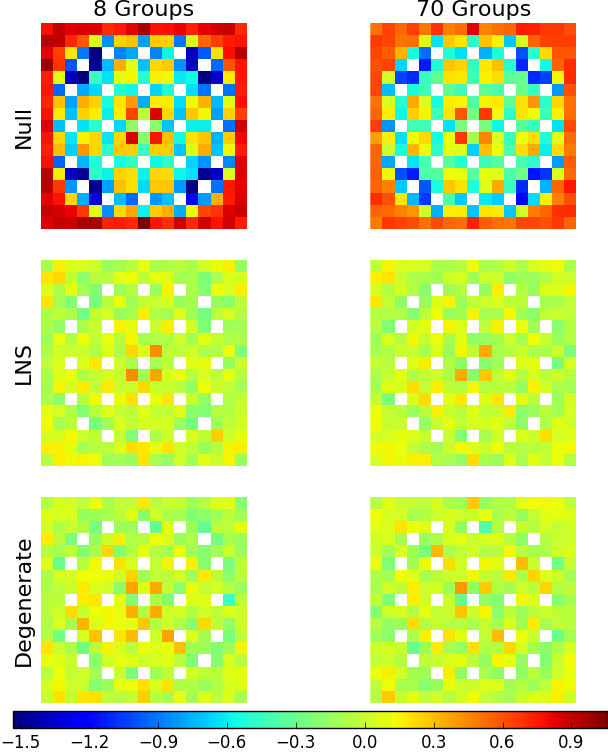
\includegraphics[width=\linewidth]{figures/patterns/lns/assm-16/capt-err}
\vspace{2mm}
\caption[U-238 capture rate errors for a 1.6\% enriched assembly]{U-238 capture rate percent relative errors errors for a 1.6\% enriched assembly with null, \ac{LNS} and degenerate spatial homogenization.}
\label{fig:chap9-assm-1.6-lns-capt-err}
\end{figure}

\clearpage

\begin{figure}[h!]
\centering
\includegraphics[width=\linewidth]{figures/patterns/lns/assm-31/capt-err}
\vspace{2mm}
\caption[U-238 capture rate errors for a 3.1\% enriched assembly]{U-238 capture rate percent relative errors errors for a 3.1\% enriched assembly with null, \ac{LNS} and degenerate spatial homogenization.}
\label{fig:chap9-assm-3.1-lns-capt-err}
\end{figure}

\clearpage

\begin{figure}[h!]
\centering
\includegraphics[width=\linewidth]{figures/patterns/lns/assm-31-20BPs/capt-err}
\vspace{2mm}
\caption[U-238 capture rate errors for a 3.1\% enriched assembly with 20 BPs]{U-238 capture rate percent relative errors errors for a 3.1\% enriched assembly with 20 \acp{BP} with null, \ac{LNS} and degenerate spatial homogenization.}
\label{fig:chap9-assm-3.1-20BPs-lns-capt-err}
\end{figure}

\clearpage

\begin{figure}[h!]
\centering
\includegraphics[width=\linewidth]{figures/patterns/lns/2x2/capt-err}
\vspace{2mm}
\caption[U-238 capture rate errors for a 2$\times$2 colorset]{U-238 capture rate percent relative errors errors for a 2$\times$2 colorset with null, \ac{LNS} and degenerate spatial homogenization.}
\label{fig:chap9-2x2-lns-capt-err}
\end{figure}

\clearpage

\begin{figure}[h!]
\centering
\includegraphics[width=\linewidth]{figures/patterns/lns/reflector/capt-err}
\vspace{2mm}
\caption[U-238 capture rate errors for a 2$\times$2 colorset with a reflector]{U-238 capture percent relative errors rate errors for a 2$\times$2 colorset with null, \ac{LNS} and degenerate spatial homogenization.}
\label{fig:chap9-reflector-lns-capt-err}
\end{figure}

\clearpage

\begin{figure}[h!]
\centering
\includegraphics[width=\linewidth]{figures/patterns/lns/full-core/capt-err-null}
\vspace{2mm}
\caption[U-238 capture rate errors for BEAVRS]{U-238 capture rate percent relative errors for the 2D quarter core \ac{BEAVRS} model with null spatial homogenization.}
\label{fig:chap9-full-core-capt-err-null}
\end{figure}

\clearpage

\begin{figure}[h!]
\centering
\includegraphics[width=\linewidth]{figures/patterns/lns/full-core/capt-err-lns}
\vspace{2mm}
\caption[U-238 capture rate errors for BEAVRS]{U-238 capture rate percent relative errors for the 2D quarter core \ac{BEAVRS} model with \ac{LNS} spatial homogenization.}
\label{fig:chap9-full-core-capt-err-lns}
\end{figure}

\clearpage

\begin{figure}[h!]
\centering
\includegraphics[width=\linewidth]{figures/patterns/lns/full-core/capt-err-degenerate}
\vspace{2mm}
\caption[U-238 capture rate errors for BEAVRS]{U-238 capture rate percent relative errors for the 2D quarter core \ac{BEAVRS} model with degenerate spatial homogenization.}
\label{fig:chap9-full-core-capt-err-degenerate}
\end{figure}

\clearpage


%%%%%%%%%%%%%%%%%%%%%%%%%%%%%%%%%%%%%%%%%%%%%%%%%%%%%%%%%%%%%%%%%%%%%%%%%%%%%%%
\section{MGXS Uncertainties and Convergence Rates}
\label{sec:chap9-convergence}

As discussed at the beginning of this chapter, there are two key objectives to \ac{MGXS} clustering -- to simultaneously approach the accuracy of degenerate homogenization and the convergence of null homogenization. The former objective was previously quantified in the context of \ac{LNS} spatial homogenization; the latter objective is the subject of this section. In particular, the particle track density within each spatially-homogenized tally volume must be increased in order to converge the statistical uncertainties faster than is possible with degenerate homogenization.

\ac{LNS} homogenization attempts to accomplish this by predicting which fuel pins have similar \ac{MGXS} and homogenizing their tally volumes into a single set of \ac{MGXS} for each set of pins with unique \ac{LNS} identifiers. This section quantifies the accelerated convergence for the \ac{LNS} scheme and contrasts it with the null and degenerate schemes. A series of OpenMC simulations were performed for each benchmark with 10,000 batches of 100,000 particles per batch for a total of 10$^{9}$ particle histories, with cumulative tally results stored every 20 batches. Stationarity of the fission source was obtained with 100 inactive batches for the assembly and colorset benchmarks; 200 inactive batches were used for the quarter core \ac{BEAVRS} model. Sec.~\ref{subsec:chap9-theory} discusses the expected difference in statistical uncertainties and convergence rates for \ac{MGXS} generated with null, degenerate and \ac{LNS} spatial homogenization. Secs.~\ref{subsec:chap9-batchwise-uncertainties} and~\ref{subsec:chap9-batchwise-deviation} present the empirical batchwise evolution of the statistical uncertainties and percent deviation for pin-wise \ac{MGXS} computed using null, degenerate and \ac{LNS} homogenization, respectively\footnote{The interested reader is referred to the work by Nelson~\cite{nelson2014improved} which performs a more detailed and systematic evaluation of the convergence of \ac{MGXS} -- most notably, scattering and fission production matrices -- which is the beyond the scope of this thesis.}.

%%%%%%%%%%%%%%%%%%%%%%%%%%%%%%%%%%%%%%%
\subsection{Theoretical Considerations}
\label{subsec:chap9-theory}

This section highlights a few theoretical considerations which should be understood when analyzing the empirical data presented in the following sections. Sec.~\ref{subsubsec:chap9-relative-uncertainties} introduces a model to predict the reduction of statistical uncertainty that can be expected with the use of \ac{LNS} spatial homogenization. Sec.~\ref{subsubsec:chap9-convergence-rates} makes a few comments about the ideal and expected convergence rate of \ac{MGXS} generated from \ac{MC} tallies.

%%%%%%%%%%%%%%%%%%%%%%%%%%%%%%%%%%%%%%%%%%%%%%%
\subsubsection{Relative Statistical Uncertainties}
\label{subsubsec:chap9-relative-uncertainties}

This section introduces a simple mathematical relation to predict the relative uncertainties for degenerate and \ac{LNS} spatial homogenization for a given number of \ac{MC} particle histories\footnote{This analysis is relevant for any scheme which uses track density-weighting to homogenize \ac{MGXS} tallied over distinct spatial volumes (\textit{e.g.}, fuel pins). This approach will be used to evaluate the unsupervised statistical clustering methodology for spatial homogenization introduced in Chaps.~\ref{chap:unsupervised} and~\ref{chap:results}.}. It should be recalled from Tab.~\ref{table:chap9-num-materials-lns} that the \ac{LNS} scheme reduced the number of materials by >25$\times$ with respect to degenerate homogenization. As a result, the particle track density within each \ac{LNS} tally volume increased according to the number of fuel pins homogenized for each unique \ac{LNS} identifier $m$, respectively. The expected (or ideal) reduction of the statistical uncertainties with \ac{LNS} homogenization may be derived from this with a few key assumptions. 

First, assume the microscopic \ac{MGXS} of the fuel pins $k \in \mathbb{S}_{m}$ with \ac{LNS} identifier $m$ are independent and identically distributed (i.i.d.) samples, each drawn from a corresponding normal distribution $\mathcal{N}(\mu_{k}, \sigma_{m}^2)$\footnote{The symbol $\sigma$ for the standard deviation should not be misconstrued for the microscopic cross section.}. The sampling distributions for the \ac{MGXS} in each fuel pin instance $k$ may have different means $\mu_{k}$, but are assumed to have the same standard deviation $\sigma_{m}$ for each \ac{LNS} identifier\footnote{The standard deviations are only the same if the track density within each fuel pin instance $i$ for each volume of phase space ($\mathbf{r},\mathbf{\Omega},E$) is identical. In this case, the standard deviations of the tallied pin-wise \ac{MGXS} would be identical. While this approximation is never true in practice, Tab.~\ref{table:chap9-std-dev-mgxs} indicates that the standard deviations for pin-wise \ac{MGXS} are only within a few multiples of one another for each of the six benchmarks (\textit{i.e.}, the standard deviations are within a narrowly dispersed ``band'').}. The standard deviations $\sigma_{\hat{\sigma}_{x,i,m,g}}$ of the homogenized microscopic \ac{MGXS} $\hat{\sigma}_{x,i,m,g}$ (Eqn.~\ref{eqn:chap9-lns-micro}) for each \ac{LNS} set $\mathbb{S}_{m}$ are then inversely proportional to the square root of the number of pins in each set:

\begin{equation}
\label{eqn:chap9-homogenize-std-dev}
\sigma_{\hat{\sigma}_{x,i,m,g}} \approx \frac{\sigma_{m}}{\sqrt{|\mathbb{S}_{m}|}}
\end{equation}

The factor $\nicefrac{\sigma_{m}}{\sqrt{|\mathbb{S}_{m}|}}$ is the expected downward ``shift'' of the standard deviation for \ac{LNS} homogenized \ac{MGXS} with respect to the degenerate \ac{MGXS}. The magnitude of the shift depends on the standard deviation $\sigma_{m}$ of the tallied \ac{MGXS} for each pin comprising the \ac{LNS} set $\mathbb{S}_{m}$, as well as the number of fuel pins $|\mathbb{S}_{m}|$ assigned to the set. The former is roughly equivalent to the tally uncertainties for the pin-wise \ac{MGXS} for degenerate homogenization and is controlled by the number of particle histories simulated for a given benchmark. The latter depends on the number of fuel pins assigned to each \ac{LNS} set, which may not be evenly distributed. For example, the individual fuel assembly with \acp{CRGT} (see Fig.~\ref{fig:chap9-assm-31-lns-materials}) has $4 \; \le \; |\mathbb{S}_{m}| \; \le \; 64$; in other words, the number of fuel pins assigned unique \ac{LNS} identifiers varies widely. As a result, the downward shift for the standard deviations of the \ac{MGXS} for each \ac{LNS} cluster will vary accordingly. For example, the standard deviations of those pins facially adjacent to a single \acp{CRGT} in the assembly benchmarks without \acp{BP} ($|\mathbb{S}_{m}| = 64$) should be reduced by approximately $\nicefrac{1}{8}$ with respect to the standard deviations of the \ac{MGXS} for each of the individual pins. The standard deviations of the pins adjacent to the central instrument tube ($|\mathbb{S}_{m}| = 4$) will only be reduced by approximately $\nicefrac{1}{2}$ since there are far fewer pins within this \ac{LNS} set.

As a result of the uneven assignment of pins to \ac{LNS} sets, the relation in Eqn.~\ref{eqn:chap9-homogenize-std-dev} is only useful to compare the relative uncertainties for the \ac{MGXS} in a single \ac{LNS} set to those of the individual pins which comprise the corresponding set. It should not be used to predict the relative uncertainties for the population of \ac{MGXS} generated from \ac{LNS} homogenization, as these cannot be generally characterized as an ensemble. Lastly, the relation may be applied to predict the relative uncertainties between null and degenerate homogenization, as is done in Sec.~\ref{subsec:chap9-batchwise-uncertainties} and benchmarked to empirical data.

%%%%%%%%%%%%%%%%%%%%%%%%%%%%%%%%%%%
\subsubsection{MGXS Convergence Rates}
\label{subsubsec:chap9-convergence-rates}

The \ac{MGXS} ``convergence rate'' as defined here refers to the reduction in the statistical uncertainties with the number of independent simulated realizations (\textit{i.e.}, \ac{MC} batches). By definition, the empirical \ac{MC} tally standard deviations will converge as $\nicefrac{1}{\sqrt{N}}$ for $N$ batches (see Sec.~\ref{subsec:chap3-mc-stats}). However, this convergence rate only holds true for \ac{MC} particle transport simulations if the tally realizations for each batch are i.i.d. Although this is the case for fixed source \ac{MC} simulations, it is not the case for eigenvalue simulations for reactor physics analysis. In particular, the correlation between the fission source distributions for successive batches is correlated in criticality calculations which breaks the independence assumption and dampens the convergence rate~\cite{herman2014correlation, miao2016correlation}. The auto-correlation coefficient between successive batches is required to account for correlations of the fission source sites in the estimated standard deviation of the mean. In general, the coefficient cannot be quantified without an ensemble of simulations, and therefore is not used here to estimate the \ac{MGXS} standard deviations. As a result, the reported standard deviations and convergence rates are likely to be under-estimated and over-estimated, respectively, especially for the high dominance ratio quarter core \ac{BEAVRS} model.

%-if we accounted for auto-correlation between batches, then the observed convergence rate would be less than ideal
%-ideal is observed for single simulation w/o accounting for auto-correlation as an optimistic estimate

%-actually, the standard deviation should converge according to the ideal rate
%  -it is only the RMS that does not converge as quickly
%-note that the ideal is only *achieved* if the auto-correlation coefficient is accounted for
%-however, it the coeff is not known with out an ensemble of simulation results
%-hence, the apparent convergence rate for a single simulation is overly optimistic, esp. for quarter core results
%-the convergence rate is not dampened as mentioned here - remove
%-move the discussion about the covariance to the preceding section

%Although the convergence rate of independent \ac{MC} tallies is dampened, it is not clear how the correlation of fission source distributions impacts the \ac{MGXS} convergence rate. Most \ac{MGXS} are computed as a reaction rate-to-flux ratio which may be less sensitive to correlation effects than the individual tallies themselves. While the individual flux and reaction rate tallies reflect the effects of correlations in their absolute magnitudes, these artificial deviations are positively correlated and should divide out in the \ac{MGXS}. In fact, if the positive correlation between reaction rate and flux tallies were accounted for when computing \ac{MGXS}, it would reduce the standard deviations through the subtraction of a positive covariance term (see Eqn.~\ref{eqn:chap3-div}). However, as discussed in Sec.~\ref{subsec:chap3-uncertainty-prop}, the tally covariance cannot be quantified without an ensemble of simulations, and therefore is not used here to reduce the \ac{MGXS} uncertainties. A few empirical case studies of the \ac{MGXS} convergence rate are highlighted in the following section, but an in-depth analysis of the interplay between fission source correlations and \ac{MGXS} convergence remains an open question for future research.

%%%%%%%%%%%%%%%%%%%%%%%%%%%%%%%%%%%%%%%%%%%%%%%%
\subsection{Batchwise Statistical Uncertainties}
\label{subsec:chap9-batchwise-uncertainties}

The statistical uncertainties for the pin-wise \ac{MGXS} were reported for the ``fully converged'' \ac{MGXS} in Sec.~\ref{subsec:chap9-mgxs-uncertainty}. The \ac{MGXS} uncertainties were computed with uncertainty propagation (see Sec.~\ref{subsec:chap3-uncertainty-prop}) of the standard deviations of the reaction rate and flux tally means (see Eqn.~\ref{eqn:chap3-variance-mean}). This section presents the evolution of those uncertainties with the number of particles simulated by OpenMC. The standard deviation of the pin-wise \ac{MGXS} for null, degenerate and \ac{LNS} homogenization were computed every 20 batches for U-235 fission and U-238 capture \ac{MGXS}. The standard deviations are plotted for the 1.6\% enriched assembly and the quarter core \ac{BEAVRS} models in Figs.~\Crefrange{fig:chap9-capt-27-var}{fig:chap9-fiss-2-var}. The evolution is shown for both the maximum and mean standard deviations of the population of \ac{MGXS} for \ac{LNS} and degenerate homogenization.

The relation in Eqn.~\ref{eqn:chap9-homogenize-std-dev} may be used to understand the relative difference (\textit{i.e.}, vertical offset) in statistical uncertainties for the three homogenization schemes. First, the relation predicts a $\sim$16$\times$ reduction of the uncertainties for the null homogenized \ac{MGXS} of the 264 pins in the 1.6\% enriched assembly with respect to the degenerate \ac{MGXS}. This compares well to the empirically observed reduction of 18 -- 22$\times$ for the the different \ac{MGXS} types. Similarly, the relation predicts a $\sim$23$\times$ reduction in the uncertainties for the null homogenized \ac{MGXS} of the 549 1.6\% enriched fuel pins in the quarter core \ac{BEAVRS} model with respect to the degenerate \ac{MGXS}. The empirically observed reduction of 18 -- 20$\times$ is smaller, most likely due to the larger disparity in the standard deviations of the \ac{MGXS} for each fuel pin, which breaks the assumption made in Sec.~\ref{subsubsec:chap9-relative-uncertainties} that the standard deviations are identical for all samples.

\begin{figure}[h!]
\centering
\begin{subfigure}{.85\textwidth}
  \centering
  \includegraphics[width=\linewidth]{figures/patterns/convergence/assm-16/assm-16-var-capture-27}
  \caption{}
  \label{fig:chap9-assm-16-var-capt-27}
\end{subfigure}
\begin{subfigure}{.85\textwidth}
  \centering
  \includegraphics[width=\linewidth]{figures/patterns/convergence/full-core/16-enr-var-capture-27}
  \caption{}
  \label{fig:chap9-full-core-var-capt-27}
\end{subfigure}
\caption[Convergence of U-238 capture MGXS standard deviation]{The standard deviation of pin-wise U-238 capture \ac{MGXS} (group 27 of 70) for 1.6\% enriched fuel pins in a single assembly (a) and the quarter core \ac{BEAVRS} model (b). The thin black dashed lines indicate the theoretical $\nicefrac{1}{\sqrt{N}}$ convergence for the maximum standard deviations of each homogenization scheme.}
\label{fig:chap9-capt-27-var}
\end{figure}

\clearpage

\begin{figure}[h!]
\centering
\begin{subfigure}{.85\textwidth}
  \centering
  \includegraphics[width=\linewidth]{figures/patterns/convergence/assm-16/assm-16-var-capture-1}
  \caption{}
  \label{fig:chap9-assm-16-var-capt-1}
\end{subfigure}
\begin{subfigure}{.85\textwidth}
  \centering
  \includegraphics[width=\linewidth]{figures/patterns/convergence/full-core/16-enr-var-capture-1}
  \caption{}
  \label{fig:chap9-full-core-var-capt-1}
\end{subfigure}
\caption[Convergence of U-238 capture MGXS standard deviation]{The standard deviation of pin-wise U-238 capture \ac{MGXS} (group 1 of 2) for 1.6\% enriched fuel pins in a single assembly (a) and the quarter core \ac{BEAVRS} model (b). The thin black dashed lines indicate the theoretical $\nicefrac{1}{\sqrt{N}}$ convergence for the maximum standard deviations of each homogenization scheme.}
\label{fig:chap9-capt-1-var}
\end{figure}

\clearpage

\begin{figure}[h!]
\centering
\begin{subfigure}{.85\textwidth}
  \centering
  \includegraphics[width=\linewidth]{figures/patterns/convergence/assm-16/assm-16-var-fission-2}
  \caption{}
  \label{fig:chap9-assm-16-var-fiss-2}
\end{subfigure}
\begin{subfigure}{.85\textwidth}
  \centering
  \includegraphics[width=\linewidth]{figures/patterns/convergence/full-core/16-enr-var-fission-2}
  \caption{}
  \label{fig:chap9-full-core-var-fiss-2}
\end{subfigure}
\caption[Convergence of U-235 fission MGXS standard deviation]{The standard deviation of pin-wise U-235 fission \ac{MGXS} (group 2 of 2) for 1.6\% enriched fuel pins in a single assembly (a) and the quarter core \ac{BEAVRS} model (b). The thin black dashed lines indicate the theoretical $\nicefrac{1}{\sqrt{N}}$ convergence for the maximum standard deviations of each homogenization scheme.}
\label{fig:chap9-fiss-2-var}
\end{figure}

\clearpage

In addition, the gap between max and mean uncertainties for the degenerate and \ac{LNS} schemes vary between the assembly and quarter core benchmarks. In particular, the max and mean uncertainties for the degenerate scheme differ by less than 10\% for the assembly, but by $\sim$2.5$\times$ for the quarter core model (this can also be seen in Tab.~\ref{table:chap9-std-dev-mgxs}). This is caused by the highly uneven fission source distribution in the quarter core model, which results in a more uneven distribution of particle track densities across the fuel pin tally volumes than in the assembly. In contrast, the max and mean uncertainties for the \ac{LNS} scheme differ by 60 -- 70\% for the assembly but by 13 -- 16$\times$ for the quarter core model. The disparity between max and mean uncertainties for \ac{LNS} homogenization is more complicated since it reflects the number of fuel pins assigned to each spatial homogenization set in addition to the uncertainties of the \ac{MGXS} for each fuel pin. 

%Finally, the convergence rate for all three homogenization schemes is very nearly the same as illustrated by the parallel lines in each plot. However, the rates are all significantly less than $\nicefrac{1}{\sqrt{N}}$ as would be expected for an ideal simulation. This may be due to the correlations of the fission source distributions.

\begin{emphbox}
\textbf{The \ac{MGXS} statistical uncertainties converge at the same rate for null, degenerate and \ac{LNS} homogenization schemes. The uncertainties for null and \ac{LNS} homogenization are smaller than those for the degenerate scheme according to the number of fuel pins assigned to each spatial homogenization set.}
\end{emphbox}

%%%%%%%%%%%%%%%%%%%%%%%%%%%%%%%%%%%%%%%%%%%%%%%%%%
\subsection{Batchwise Relative Percent Deviations}
\label{subsec:chap9-batchwise-deviation}

The statistical uncertainties presented in the preceding section estimate the amount by which \ac{MGXS} may vary from their tallied means. However, the uncertainties do little to indicate the degree by which one may expect the solutions from a multi-group calculation to change from batch-to-batch of the \ac{MC} simulation. This section seeks to quantify the impact of \ac{MGXS} convergence on downstream codes by presenting the batchwise relative percentage deviation for \ac{MGXS} with null, degenerate and \ac{LNS} spatial homogenization. 

The batchwise relative percentage deviation quantifies the change in cumulative \ac{MGXS} estimates between two batches. The absolute batchwise relative deviation as employed here is computed for the cumulatively estimated microscopic \ac{MGXS} $\hat{\sigma}_{x,i,k,g}^{b}$ and $\hat{\sigma}_{x,i,k,g}^{b+\Delta b}$ for batches $b$ and $b + \Delta b$ as follows:

\begin{equation}
\label{eqn:chap9-batchwise-deviation}
\Delta \hat{\sigma}_{x,i,k,g} [\%] = \left|\frac{\hat{\sigma}_{x,i,k,g}^{b} - \hat{\sigma}_{x,i,k,g}^{b+\Delta b}}{\hat{\sigma}_{x,i,k,g}^{b}}\right| \times 100
\end{equation}

\noindent The batchwise relative deviation indicates the degree by which the \ac{MGXS} estimates change with the number of \ac{MC} particle histories simulated. The \ac{MGXS} estimates from batch-to-batch follow a random walk with steps which are increasingly attenuated with the number of batches. The degree of change between batches depends on the particle track density within each tally volume, and therefore should be ordered from least to greatest for null, \ac{LNS} and degenerate homogenization.

Due to computational resource constraints, the batchwise deviations were computed every $\Delta b$ = 20 batches for each \ac{MC} simulation. The absolute relative batchwise percentage deviations are plotted for the 1.6\% enriched assembly and quarter core \ac{BEAVRS} models in Figs.~\Crefrange{fig:chap9-capt-27-dev}{fig:chap9-fiss-2-dev}. The evolution is shown for both the maximum and mean deviations of the population of \ac{MGXS} for \ac{LNS} and degenerate homogenization.

\begin{figure}[h!]
\centering
\begin{subfigure}{.87\textwidth}
  \centering
  \includegraphics[width=\linewidth]{figures/patterns/convergence/assm-16/assm-16-dev-capture-27}
  \caption{}
  \label{fig:chap9-assm-16-dev-capt-27}
\end{subfigure}
\begin{subfigure}{.87\textwidth}
  \centering
  \includegraphics[width=\linewidth]{figures/patterns/convergence/full-core/16-enr-dev-capture-27}
  \caption{}
  \label{fig:chap9-full-core-dev-capt-27}
\end{subfigure}
\caption[Convergence of U-238 capture MGXS batchwise deviation]{The absolute relative batchwise percentage deviation of pin-wise U-238 capture \ac{MGXS} (group 27 of 70) for 1.6\% enriched fuel pins in a single assembly (a) and the quarter core \ac{BEAVRS} model (b).}
\label{fig:chap9-capt-27-dev}
\end{figure}

\begin{figure}[h!]
\centering
\begin{subfigure}{.87\textwidth}
  \centering
  \includegraphics[width=\linewidth]{figures/patterns/convergence/assm-16/assm-16-dev-capture-1}
  \caption{}
  \label{fig:chap9-assm-16-dev-capt-1}
\end{subfigure}
\begin{subfigure}{.87\textwidth}
  \centering
  \includegraphics[width=\linewidth]{figures/patterns/convergence/full-core/16-enr-dev-capture-1}
  \caption{}
  \label{fig:chap9-full-core-dev-capt-1}
\end{subfigure}
\caption[Convergence of U-238 capture MGXS batchwise deviation]{The absolute relative batchwise percentage deviation of pin-wise U-235 fission \ac{MGXS} (group 1 of 2) for 1.6\% enriched fuel pins in a single assembly (a) and the quarter core \ac{BEAVRS} model (b).}
\label{fig:chap9-capt-1-dev}
\end{figure}

\begin{figure}[h!]
\centering
\begin{subfigure}{.87\textwidth}
  \centering
  \includegraphics[width=\linewidth]{figures/patterns/convergence/assm-16/assm-16-dev-fission-2}
  \caption{}
  \label{fig:chap9-assm-16-dev-fiss-2}
\end{subfigure}
\begin{subfigure}{.87\textwidth}
  \centering
  \includegraphics[width=\linewidth]{figures/patterns/convergence/full-core/16-enr-dev-fission-2}
  \caption{}
  \label{fig:chap9-full-core-dev-fiss-2}
\end{subfigure}
\caption[Convergence of U-235 fission MGXS batchwise deviation]{The absolute relative batchwise percentage deviation of pin-wise U-235 fission \ac{MGXS} (group 2 of 2) for 1.6\% enriched fuel pins in a single assembly (a) and the quarter core \ac{BEAVRS} model (b).}
\label{fig:chap9-fiss-2-dev}
\end{figure}

A couple of observations can be made from the figures. First, the convergence rate (or log-log slope) of the batchwise deviations is very nearly the same for all three homogenization schemes. More importantly, however, the deviations are smallest for null homogenization and greatest for degenerate homogenization, as expected. This is manifested as a downward shift in the deviations for a given number of particle histories, and is due to the differential particle track density within each tally volume for the different homogenization schemes. The magnitude of the shift depends on the number of pins being averaged across, and is hence the greatest for the null and degenerate schemes for the quarter core \ac{BEAVRS} model, where nearly 4,500 pins of each enrichment are averaged together for the null case (as compared to only 264 pins for the assembly). In contrast, the degenerate and \ac{LNS} schemes are shifted by nearly the same amount for both benchmark models since the number of fuel pins averaged across for each \ac{LNS} set is the same. These observations confirm that the more fuel pins that are homogenized together for \ac{MGXS} clustering, the faster the resultant \ac{MGXS} tally estimates will converge for use in multi-group codes.

These results point to the need for a scheme that can effectively model \ac{MGXS} clustering in a more scalable fashion than \ac{LNS} homogenization. \ac{LNS} homogenization achieves little relative improvement in convergence of the batchwise deviations relative to the null and degenerate schemes since the pins in each fuel assembly are homogenized separately. The analysis of \ac{MGXS} clustering in Sec.~\ref{sec:chap9-clustering} indicated that fuel pins in many different assemblies may be effectively homogenized together while still accounting for clustering due to spatial self-shielding effects. This would increase the number of pins within each homogenization set and improve the convergence rate beyond what is achievable with \ac{LNS}. The following chapter introduces a novel methodology based on unsupervised statistical clustering algorithms which seeks to outperform both the accuracy and the convergence of \ac{LNS} homogenization.

\begin{emphbox}
\textbf{As with the statistical uncertainties, the \ac{MGXS} batchwise deviations converge at the same rate for null, degenerate and \ac{LNS} homogenization schemes. The relative difference in deviations between schemes is reduced according to the number of fuel pins assigned to each spatial homogenization set.}
\end{emphbox}

%third paragraph: segue into next chapter
%-goal should be to best identify groups of pins with like \ac{MGXS}
%-\ac{LNS} was used as one scheme
%  -demonstrated promise for simple benchmarks
%  -illustrated shortcomings for benchmarks with complicated heterogeneties
%    -assembly-assembly and assembly-reflector interfaces
%  -algorithm could be tweaked to pick up on these effects
%    -customizations highly reactor dependent - NOT reactor agnostic
%-would be nice to identify adequate pin groupings directly from structural patterns in the \ac{MGXS} data
%-will do this in the following chapter

\clearpage

\vfill
\begin{highlightsbox}[frametitle=Highlights]
\begin{itemize}
  \item \ac{MGXS} data for each of the six heterogeneous benchmarks was analyzed to show that spatial heterogeneities induce \ac{MGXS} \textit{dispersion} and \textit{clustering}.
%  \item It is hypothesized that \ac{MGXS} clustering must be appropriately modeled to accurately predict U-238 capture rates in heterogeneous geometries.
  \item Degenerate homogenization accounts for \ac{MGXS} clustering, but requires a large number of \ac{MC} particle histories to converge \ac{MGXS}.
  \item The \ac{LNS} spatial homogenization scheme is introduced which assigns fuel pins with similar neighbors to the same spatial homogenization set.
%  \begin{itemize}
%    \item \ac{LNS} homogenization assigns fuel pins with similar neighbors to the same spatial homogenization set.
%    \item Unique \ac{MGXS} are homogenized for the pins comprising each set.
% \end{itemize}
  \item The six benchmarks are modeled with \ac{MGXS} generated by the \ac{LNS} scheme:
  \begin{itemize}
    \item \textit{Eigenvalues} -- \ac{LNS} has no systematic impact on the eigenvalues due to the preservation of global reactivity.
    \item \textit{Fission Rates} -- \ac{LNS} performs slightly better than degenerate homogenization, which is only marginally better than the null scheme, since the fission rate predictions are largely insensitive to \ac{MGXS} clustering.
    \item \textbf{\textit{U-238 Capture Rates} -- \ac{LNS} reduces the error by 10 -- 30\% as compared to degenerate homogenization} for assembly and periodic colorset benchmarks. However, \ac{LNS} fails to distinguish between pins at inter-assembly and assembly-reflector interfaces which results in a systematically large reaction rate error for these fuel pins.
  \end{itemize}
  \item A series of case studies illustrate the need to homogenize across many fuel pins to reduce the \ac{MGXS} statistical uncertainties and batchwise deviations.
%  \item \ac{LNS} only reduces the number of materials by $\sim$25$\times$.
  \item An improved methodology is needed which can:
  \begin{itemize}  
     \item \textbf{Model arbitrary \ac{MGXS} clustering} from all spatial self-shielding effects.
     \item \textbf{Minimize the \# of materials} to improve \ac{MGXS} statistical uncertainties.
   \end{itemize}
\end{itemize}
\end{highlightsbox}
\vfill
